\documentclass[twocolumn,aps,prd,reprint]{revtex4-1}
\usepackage{blindtext, amssymb, amsmath, graphicx, commath, indentfirst, subfigure, float, fancyhdr, color, listings, geometry, hyperref, multirow}
%\usepackage[justification=centering]{caption}
\usepackage{graphics,setspace,enumitem,graphicx,textpos,placeins,float}
\begin{document}
\graphicspath{{GillianKopp/}}
\bibliographystyle{plain}
\title{Precision Timing Studies for the High Granularity Calorimeter Using a Dedicated Timing Layer}
\author{Gillian Kopp}
\email{gkopp@caltech.edu}
\author{Artur Apresyan}
\author{Javier Duarte}
\author{Cristian Pena}
\author{Maria Spiropulu}
\author{Si Xie}
\affiliation{California Institute of Technology}
%\begin{spacing}{1.2}

\begin{abstract}
The Compact Muon Solenoid (CMS) experiment records data from proton-proton (pp) collisions at the Large Hadron Collider (LHC) to study physics beyond the standard model. In order to fully exploit the sensitivity of the CMS experiment the current detectors have to be upgraded and equipped with enhanced capabilities to reduce effects of the large increase in the number of pileup interactions predicted to occur in HL-LHC program. New capabilities, such as precision timing measurement in calorimetric devices, have been shown to effectively mitigate the effects due to pileup. We present results obtained using a dedicated timing silicon layer identical to that proposed to be used in the High Granularity Calorimeter for CMS. This timing layer (pico-sil detector) was tested with high energy electromagnetic showers produced by electrons at the Fermilab Test Beam Facility. An outstanding time resolution of less than 16 ps was measured for a beam energy of 32 GeV.
\end{abstract}

\maketitle
\section{Introduction}


The Compact Muon Solenoid (CMS) experiment records data from proton-proton (pp) collisions at the Large Hadron Collider (LHC) to study physics beyond the standard model. Upgrades to the LHC, such as the High Luminosity Large Hadron Collider (HL-LHC), as well as future colliders such as the Future Circular Collider (FCC) will have a higher rate of proton collisions and will be able to produce data from more particles at higher energy. This will allow for measuring known fundamental particle properties more precisely, and for a greater capability to search for physics beyond the standard model. However, the increased rate of proton collisions requires that the current detectors must be upgraded. In the collider, a ``bunch'' (amount of protons in a beam pulse) of protons is accelerated by an EM field, with each bunch spaced out by 25 ns. When the bunch collides, there are many interactions, and the vertex of the ``main interaction'', the one with the largest amount of transverse momentum, must be identified such that the jets are associated with the correct event.

The High Luminosity upgrade will increase the luminosity by 5-10 times the current value, which will lead to 10 times the number of interaction events \cite{Bilki}. With the HL-LHC, the number of protons per bunch will be increased from $10^{11}$ to $10^{13}$ protons on average, meaning that in a collision interaction, there will be around 200 proton interactions (vs. 20-40 proton interactions with the current 13 TeV beam at the LHC). The data gathered will be from multiple proton collisions (called a pile-up collision), and the detectors need to be able to differentiate which collision each decay profile originated from. Therefore, due to the increased number of collisions, the reconstruction algorithms currently in use will not be as effective, and thus the capabilities of the detectors must be improved.

Particle detectors give information to determine specific collision vertices, as this is how rarer processes are detected (the creation of mesons, W and Z bosons, Higgs boson, and potential super-symmetric particles or dark matter). At these higher collision rates, the spatial resolution of the collision vertex can be increased either by improving the detector capabilities (detectors with finer granularity have a better spatial resolution) or by using precision timing detectors, employing time-of-flight (TOF) techniques. This research focuses on precision timing detectors used to measure the time stamp of the particle at the interaction point so the collision vertex it originated from can be traced back to for event reconstruction \cite{Xie}. The goal is to analyze the timing capabilities of these types of calorimeters and to achieve a time resolution on the order of 30 ps, as this will allow for 1 cm spacial resolution \cite{Xie}.

The HL-LHC and Phase II upgrades of the CMS detectors are scheduled for 2023, and prior to the upgrade, the detectors must be replaced and improved \cite{Bilki}. The High Granularity Calorimeter (HGC) is the chosen design for the CMS Phase II Detector Upgrade and is designed to have detector layers with high granularity due to the hexagonal silicon sensors \cite{Bilki}. The HGC will replace the current ECal (Electromagnetic Calorimeter) endcap of the CMS detector, which currently has a time resolution of 150 ps. Thus, the goal of this work is to investigate the time resolution capabilities of a HGC. Additionally, the HGC will used a SKIROC (Silicon Kalorimeter Integrated ReadOut Chip) chip for analog to digital signal conversion in the CMS upgrade, and the effects of this chip are considered in this analysis \cite{Callier}.

For this investigation, detectors were tested in the MTest beamline at Fermi National Accelerator Lab (Fermilab) with proton and electron beams from 4-32 GeV during the June 2016 Test Beam. To test the capabilities and limitations of a HGC detector, we used a silicon detector designed with hexagonal silicon ``pixels'' [Figure \ref{pico-sil}]. This dedicated silicon timing layer is identical to that proposed to be used in the HGC at CMS, and we measured its intrinsic time resolution and limitations. This detector, referred to as pico-sil (picosecond timing silicon detector) was built by engineers at Fermilab. The pico-sil detector was set up with a DRS4 for signal digitization, and thus does not use the same SKIROC chip as the HGC detector at CMS will. Therefore, the effect of the SKIROC chip was modeled based on a time smearing of the pico-sil data to investigate the time resolution of HGC detectors with use of a SKIROC2 chip.

Data from the June Fermilab beam line test with the detector prototypes has been analyzed to determine the time resolution the HGC detector can achieve, and what the limitations are. During the beamline test, we used the MTest beamline with proton and electron beams of varying energies. The analysis of the time resolution of the detectors is done by observing how the shower from an electron beam propagates through the detectors and how the signal is picked up and amplified by the multi-channel plates and silicon sensor. The detectors used are shown in Figure \ref{detectors}, and this analysis focuses on the transverse analysis of the pico-sil detector.

\begin{figure}[!htbp]
\centering
\subfigure[Diagram of the pixels in the pico-sil detector. The pixels are in a hexagonal arrangement, and the beam is focused on the center pixel (labeled \#1).]{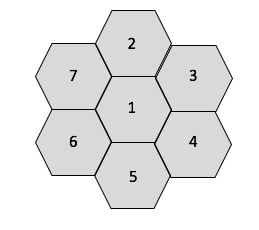
\includegraphics[width = 0.35\textwidth]{pico-sil_hexagon}} 
\subfigure[A single pixel in the pico-sil detector. The diagonal (marked with a dashed line) of each hexagon is 1cm.]{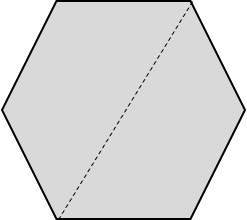
\includegraphics[width = 0.2\textwidth]{picosil_diagonal}} 
\hspace{4mm}
\subfigure[The silicon sensor electronics used for the HGC. The silicon sensor was bonded to an electronic readout board for the experiment.]{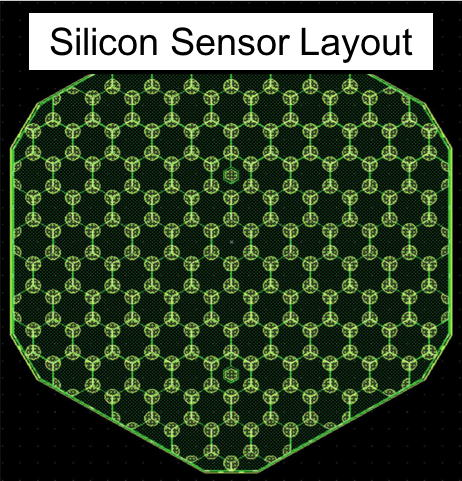
\includegraphics[width = 0.2\textwidth]{silicon_sensor}} 
\caption{Diagrams of the pico-sil detector and the hexagonal arrangement of the pixel electronics.}
\label{pico-sil}
\end{figure}

\begin{figure*}[!htbp]
\centering
\subfigure[Silicon pad detector.]{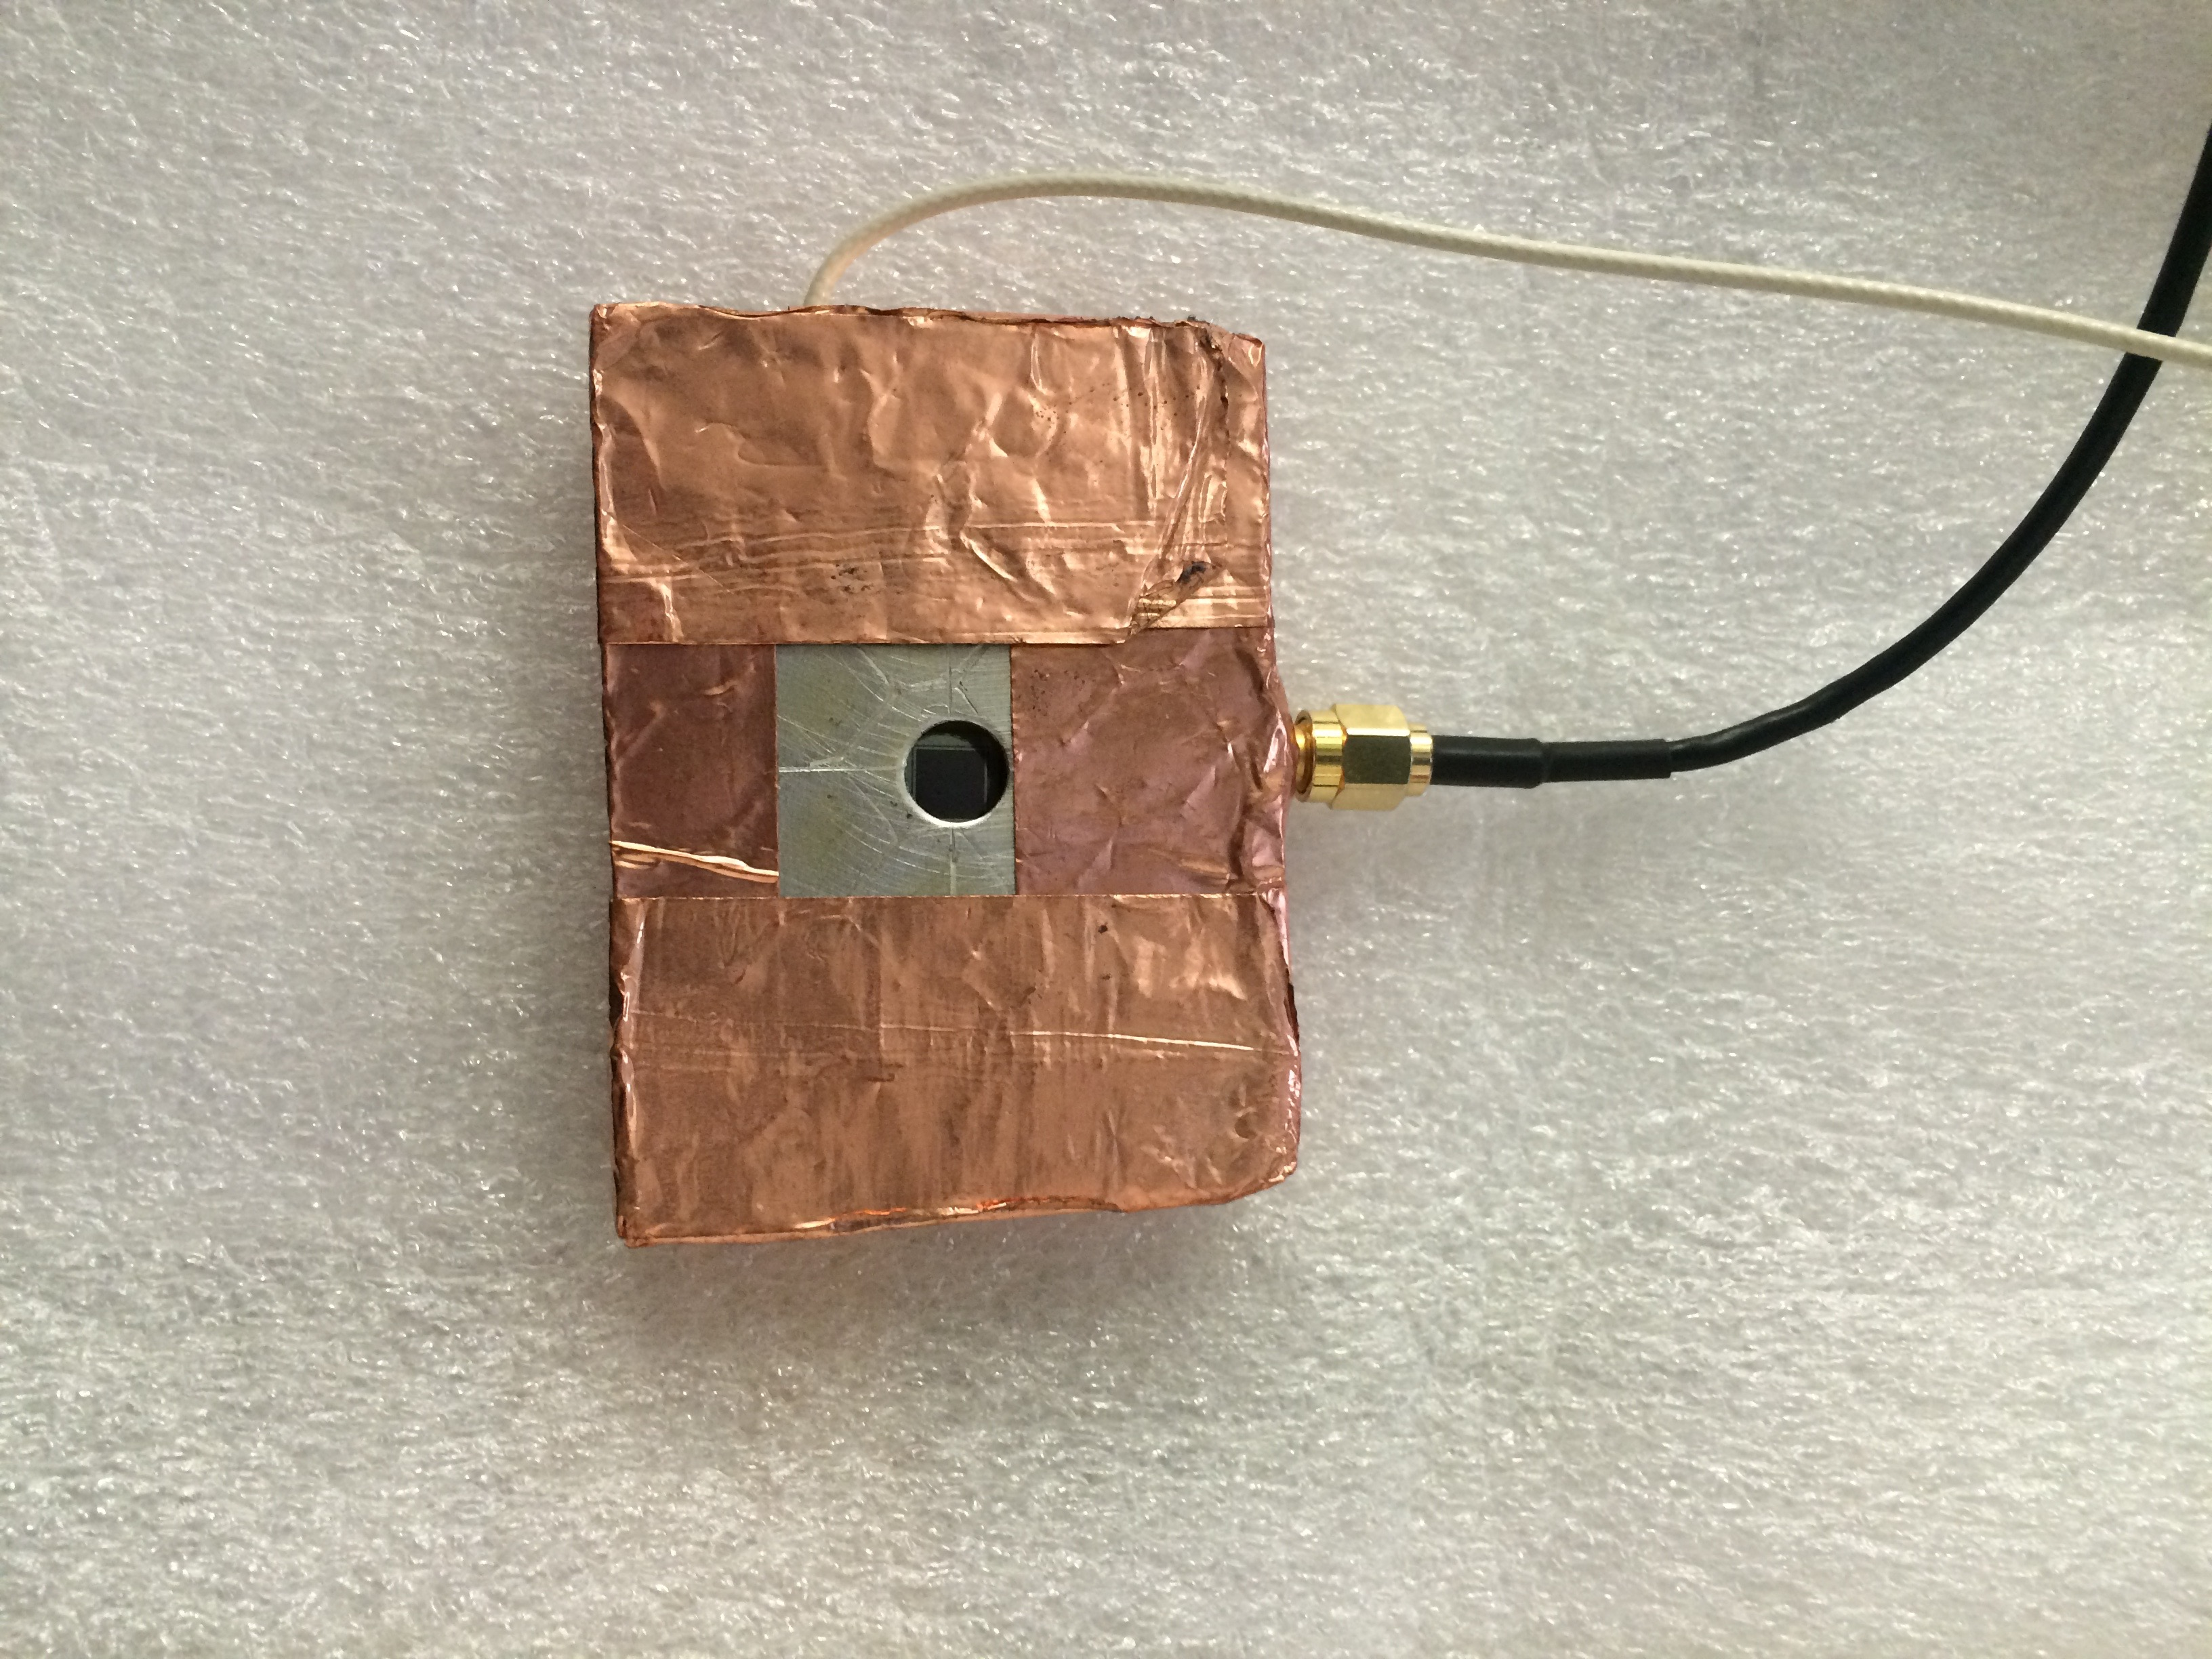
\includegraphics[width = 0.3\textwidth]{silicon-pad}} 
\subfigure[Photonis single channel detector.]{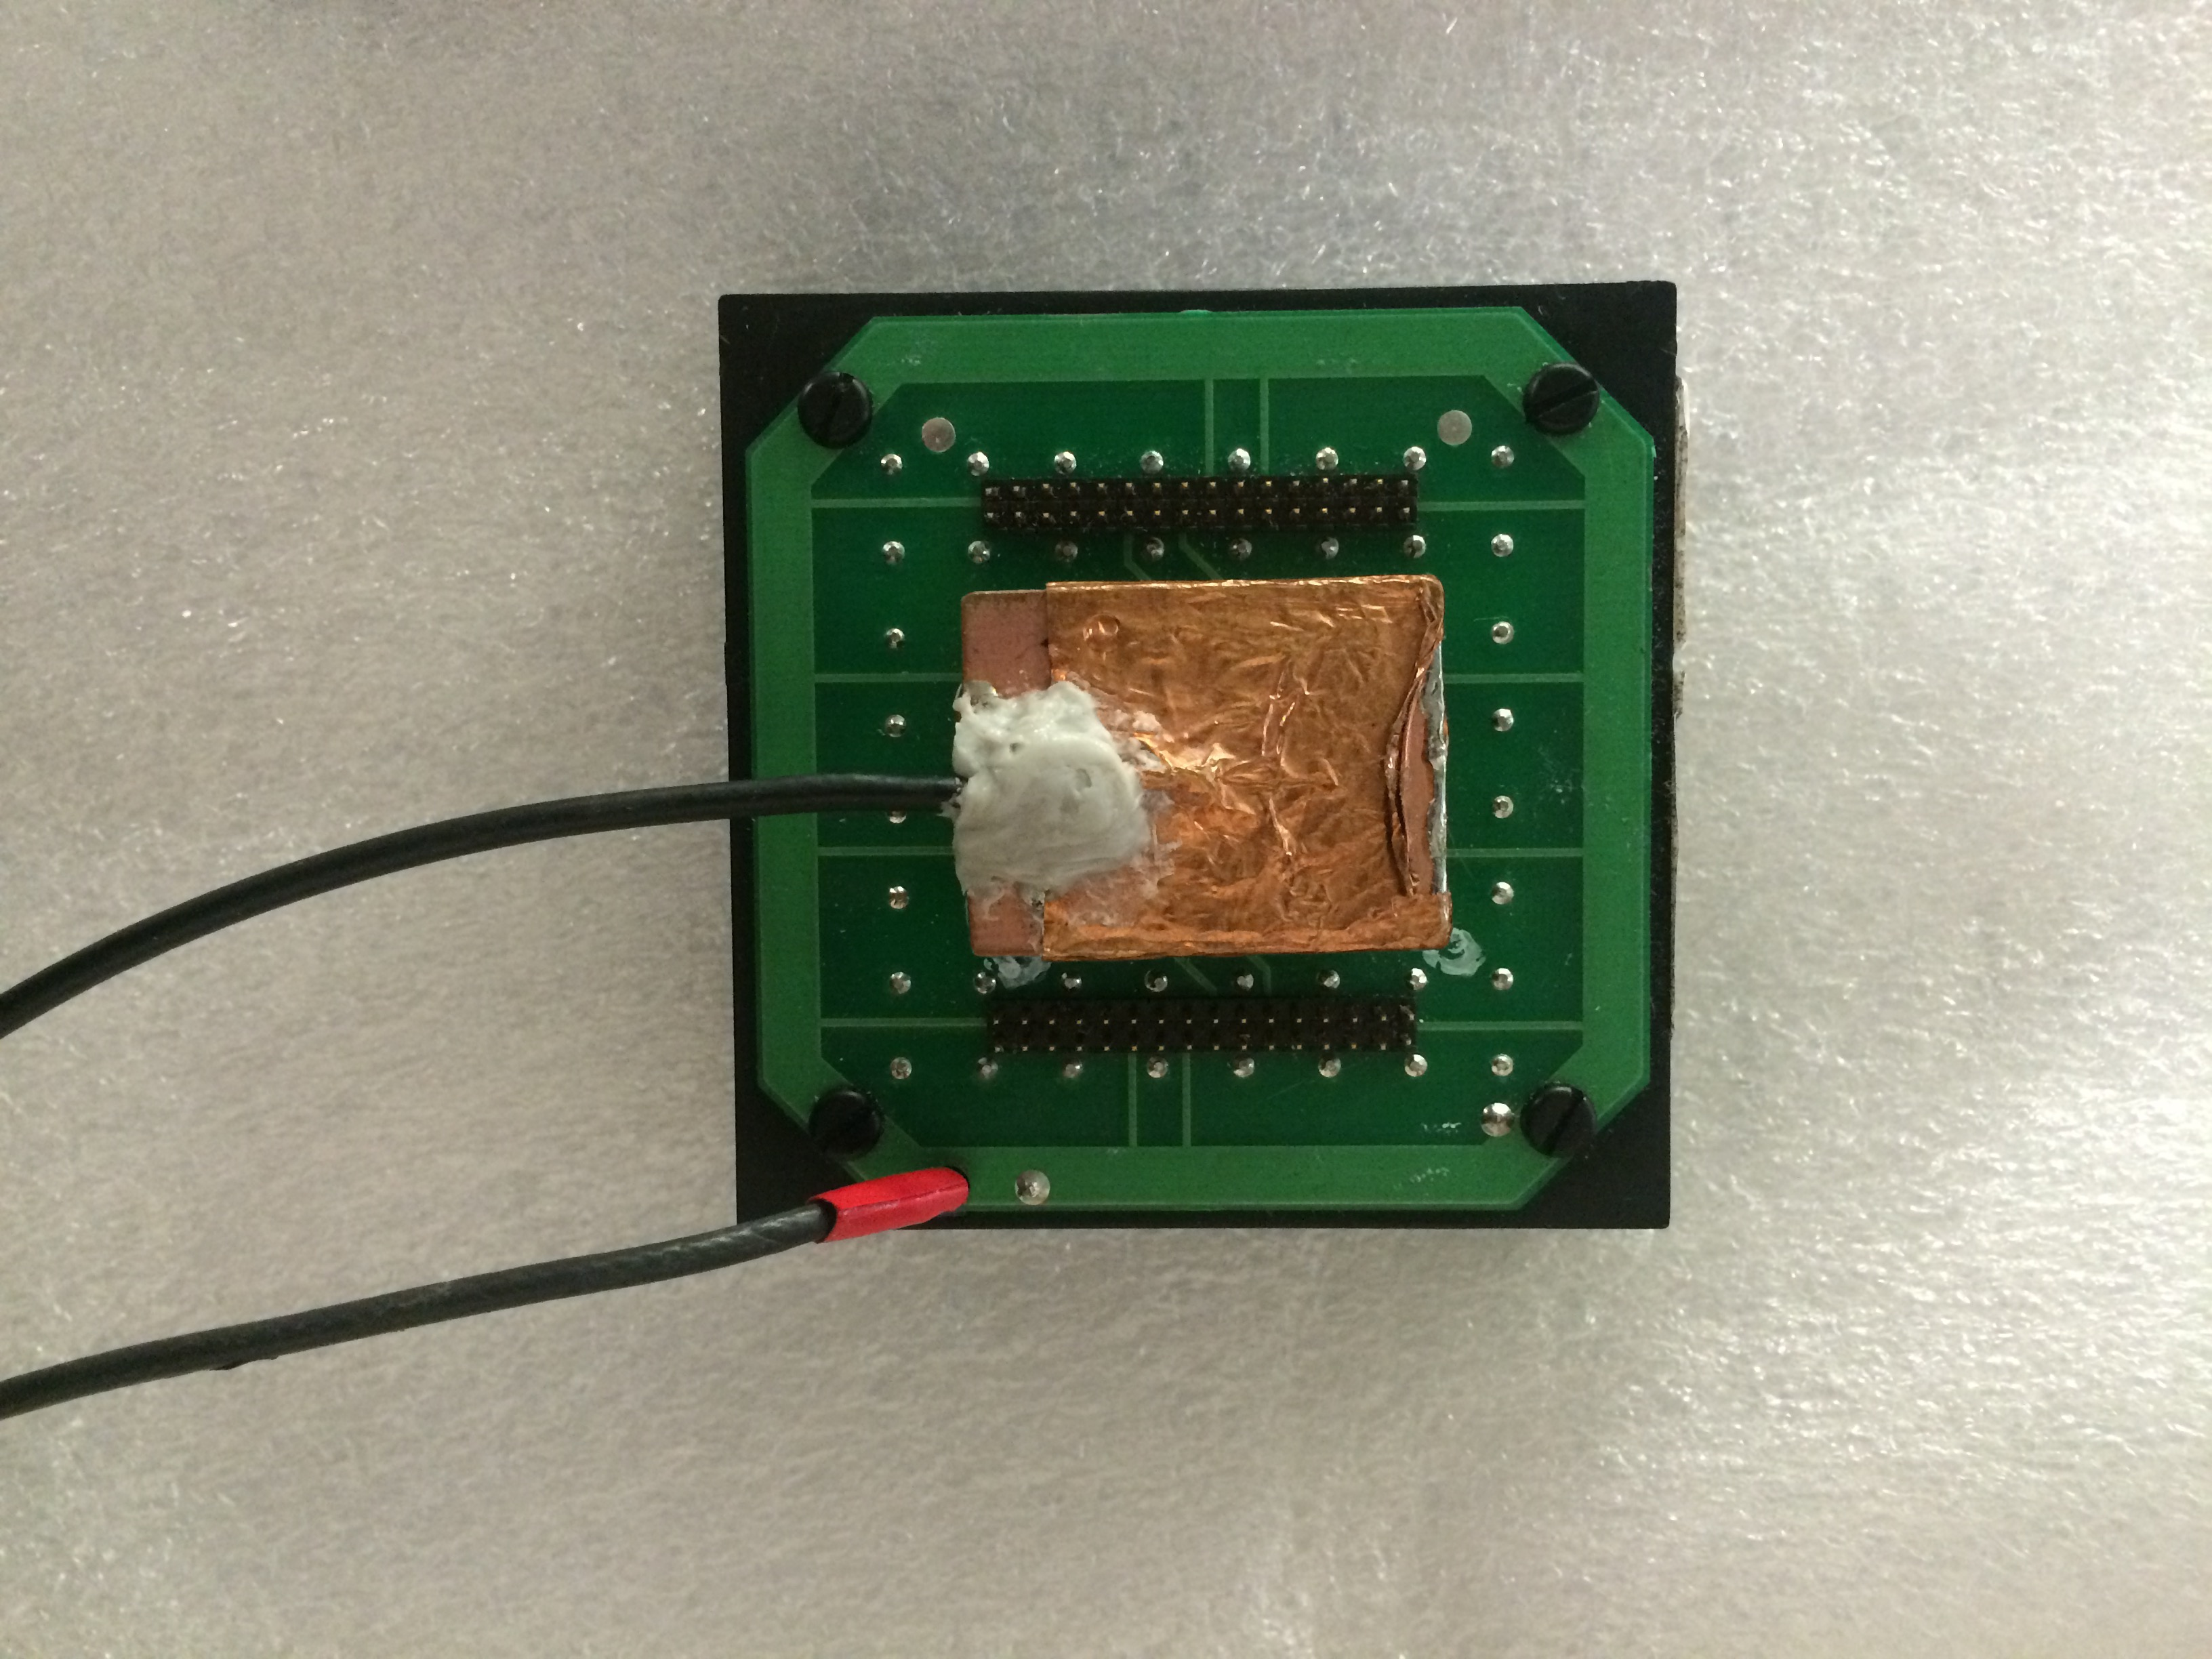
\includegraphics[width = 0.3\textwidth]{photonis}}
\subfigure[Photonis 64 channel detector, MCP-PMT (microchannel plate photo multiplier), side view.]{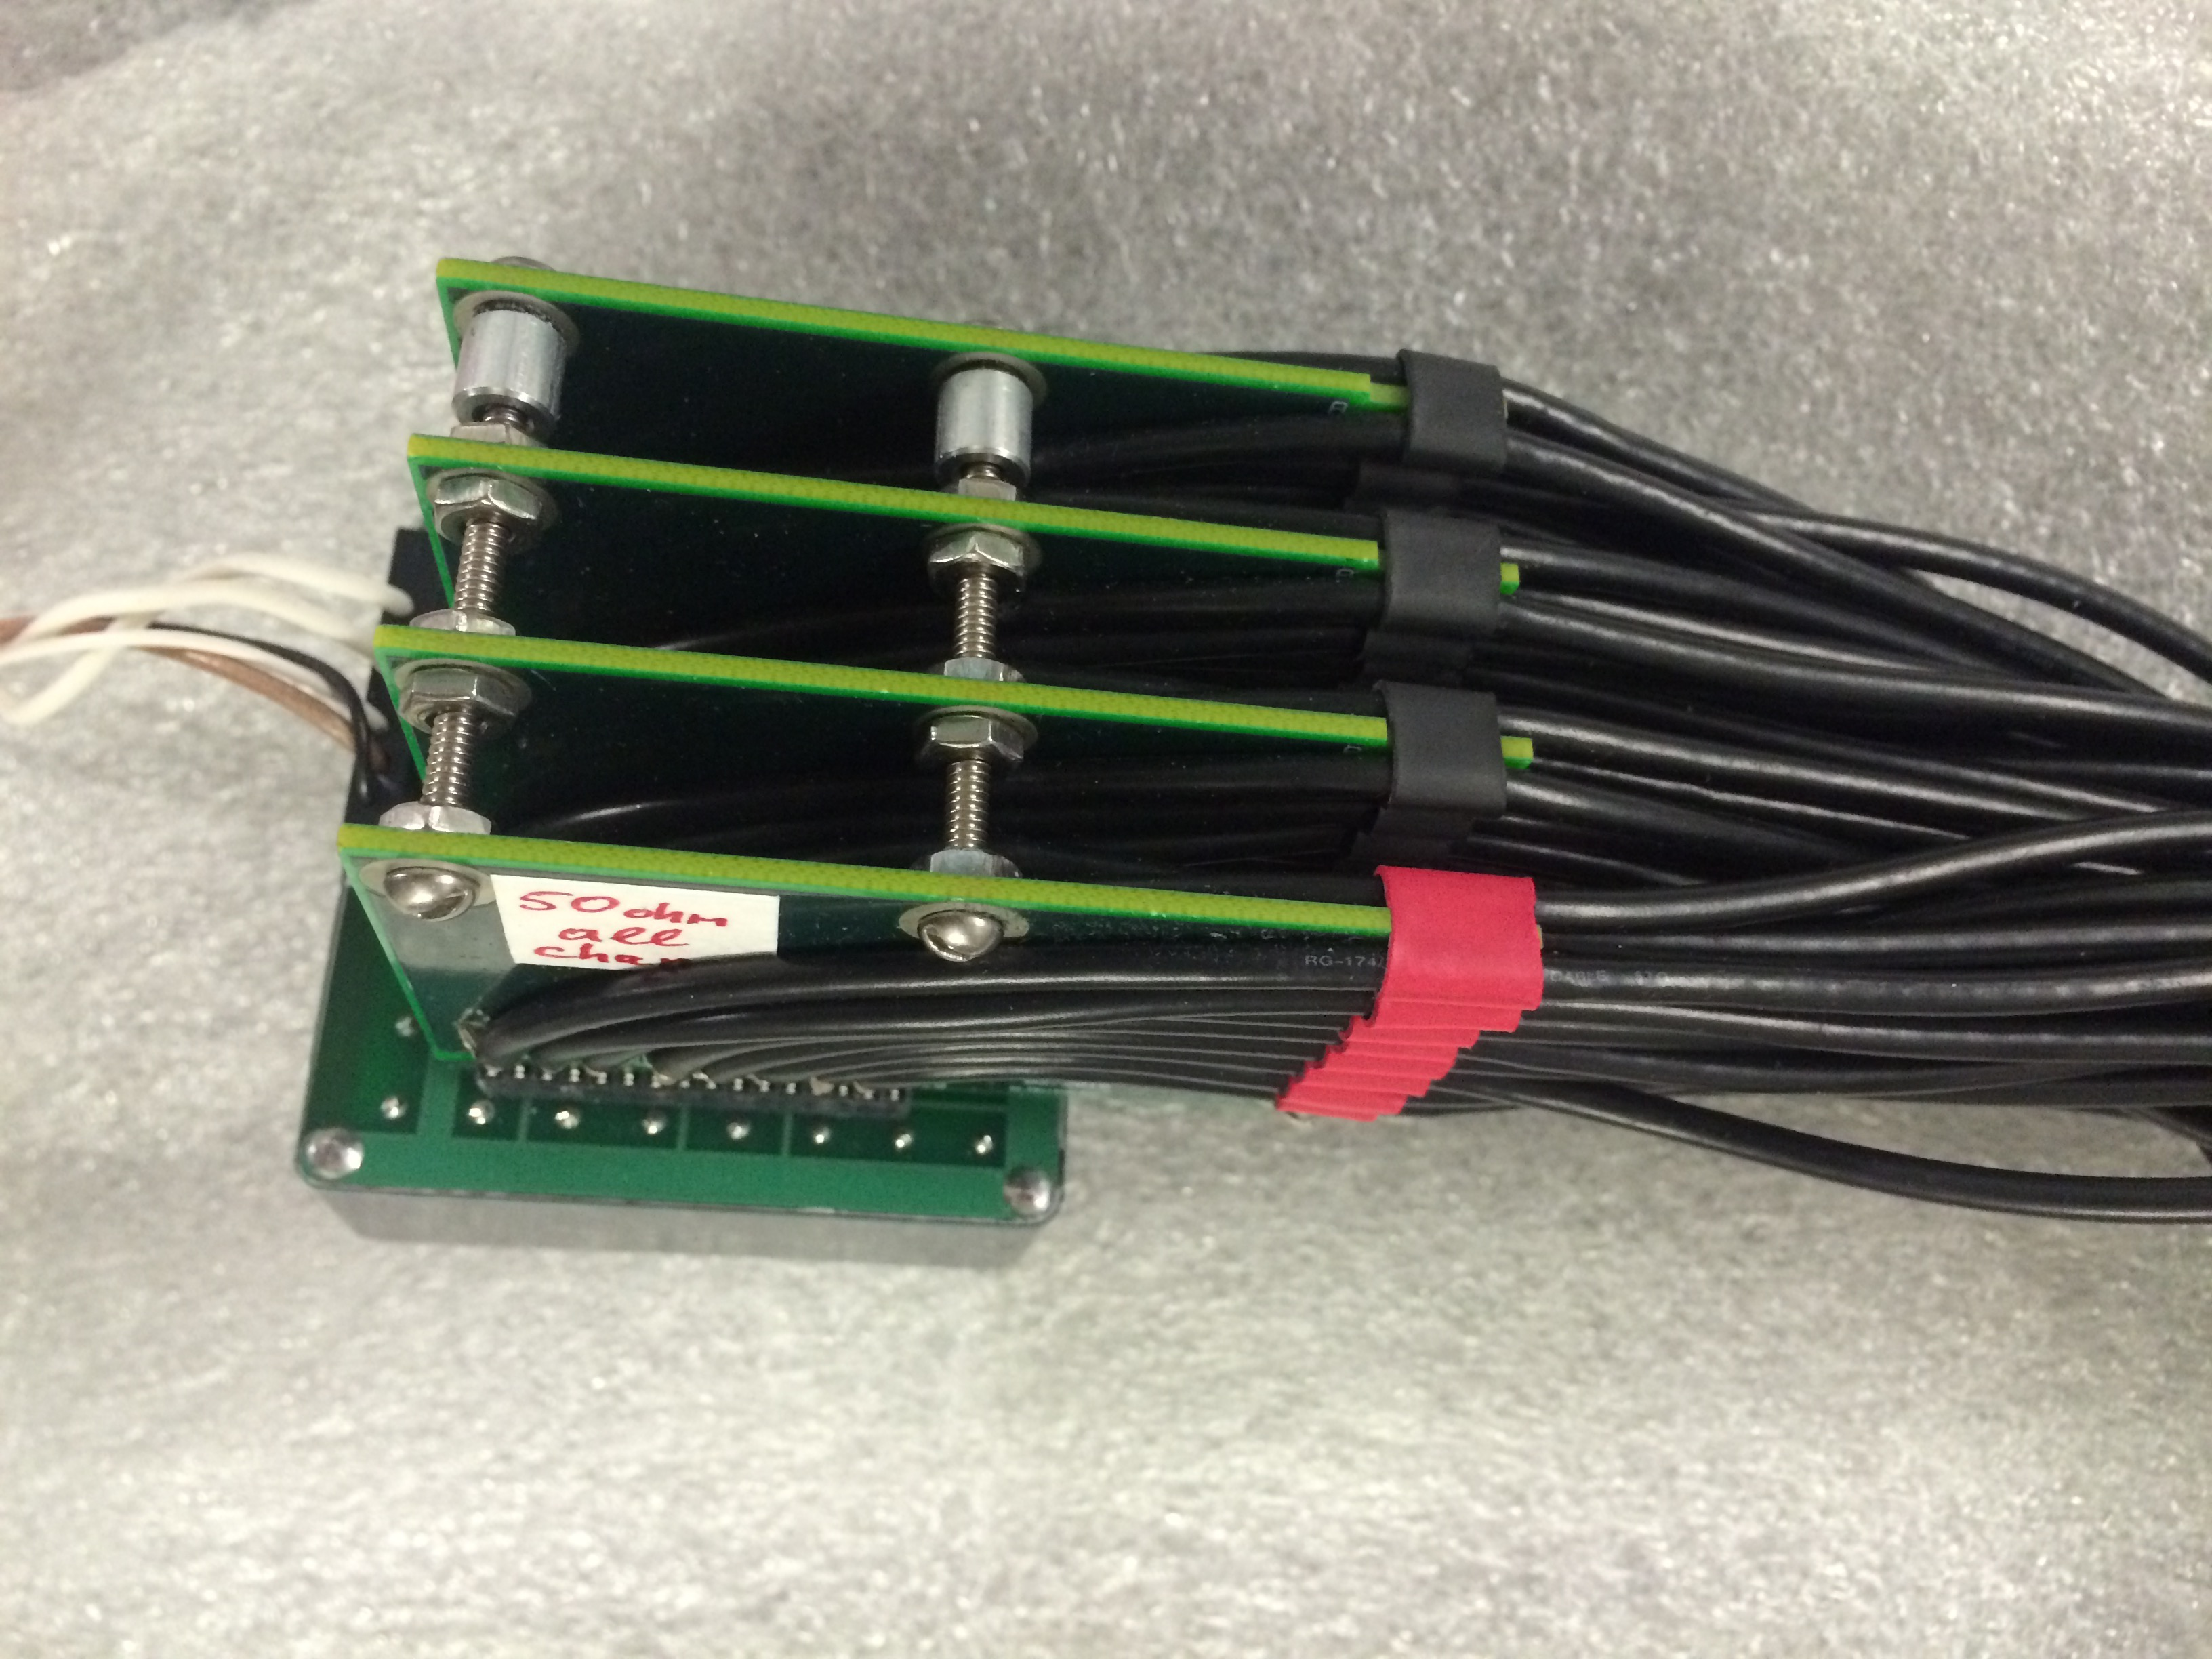
\includegraphics[width = 0.3\textwidth]{photonis64_2}} 
\subfigure[Photek detector, with the black covering to block out background light visible.]{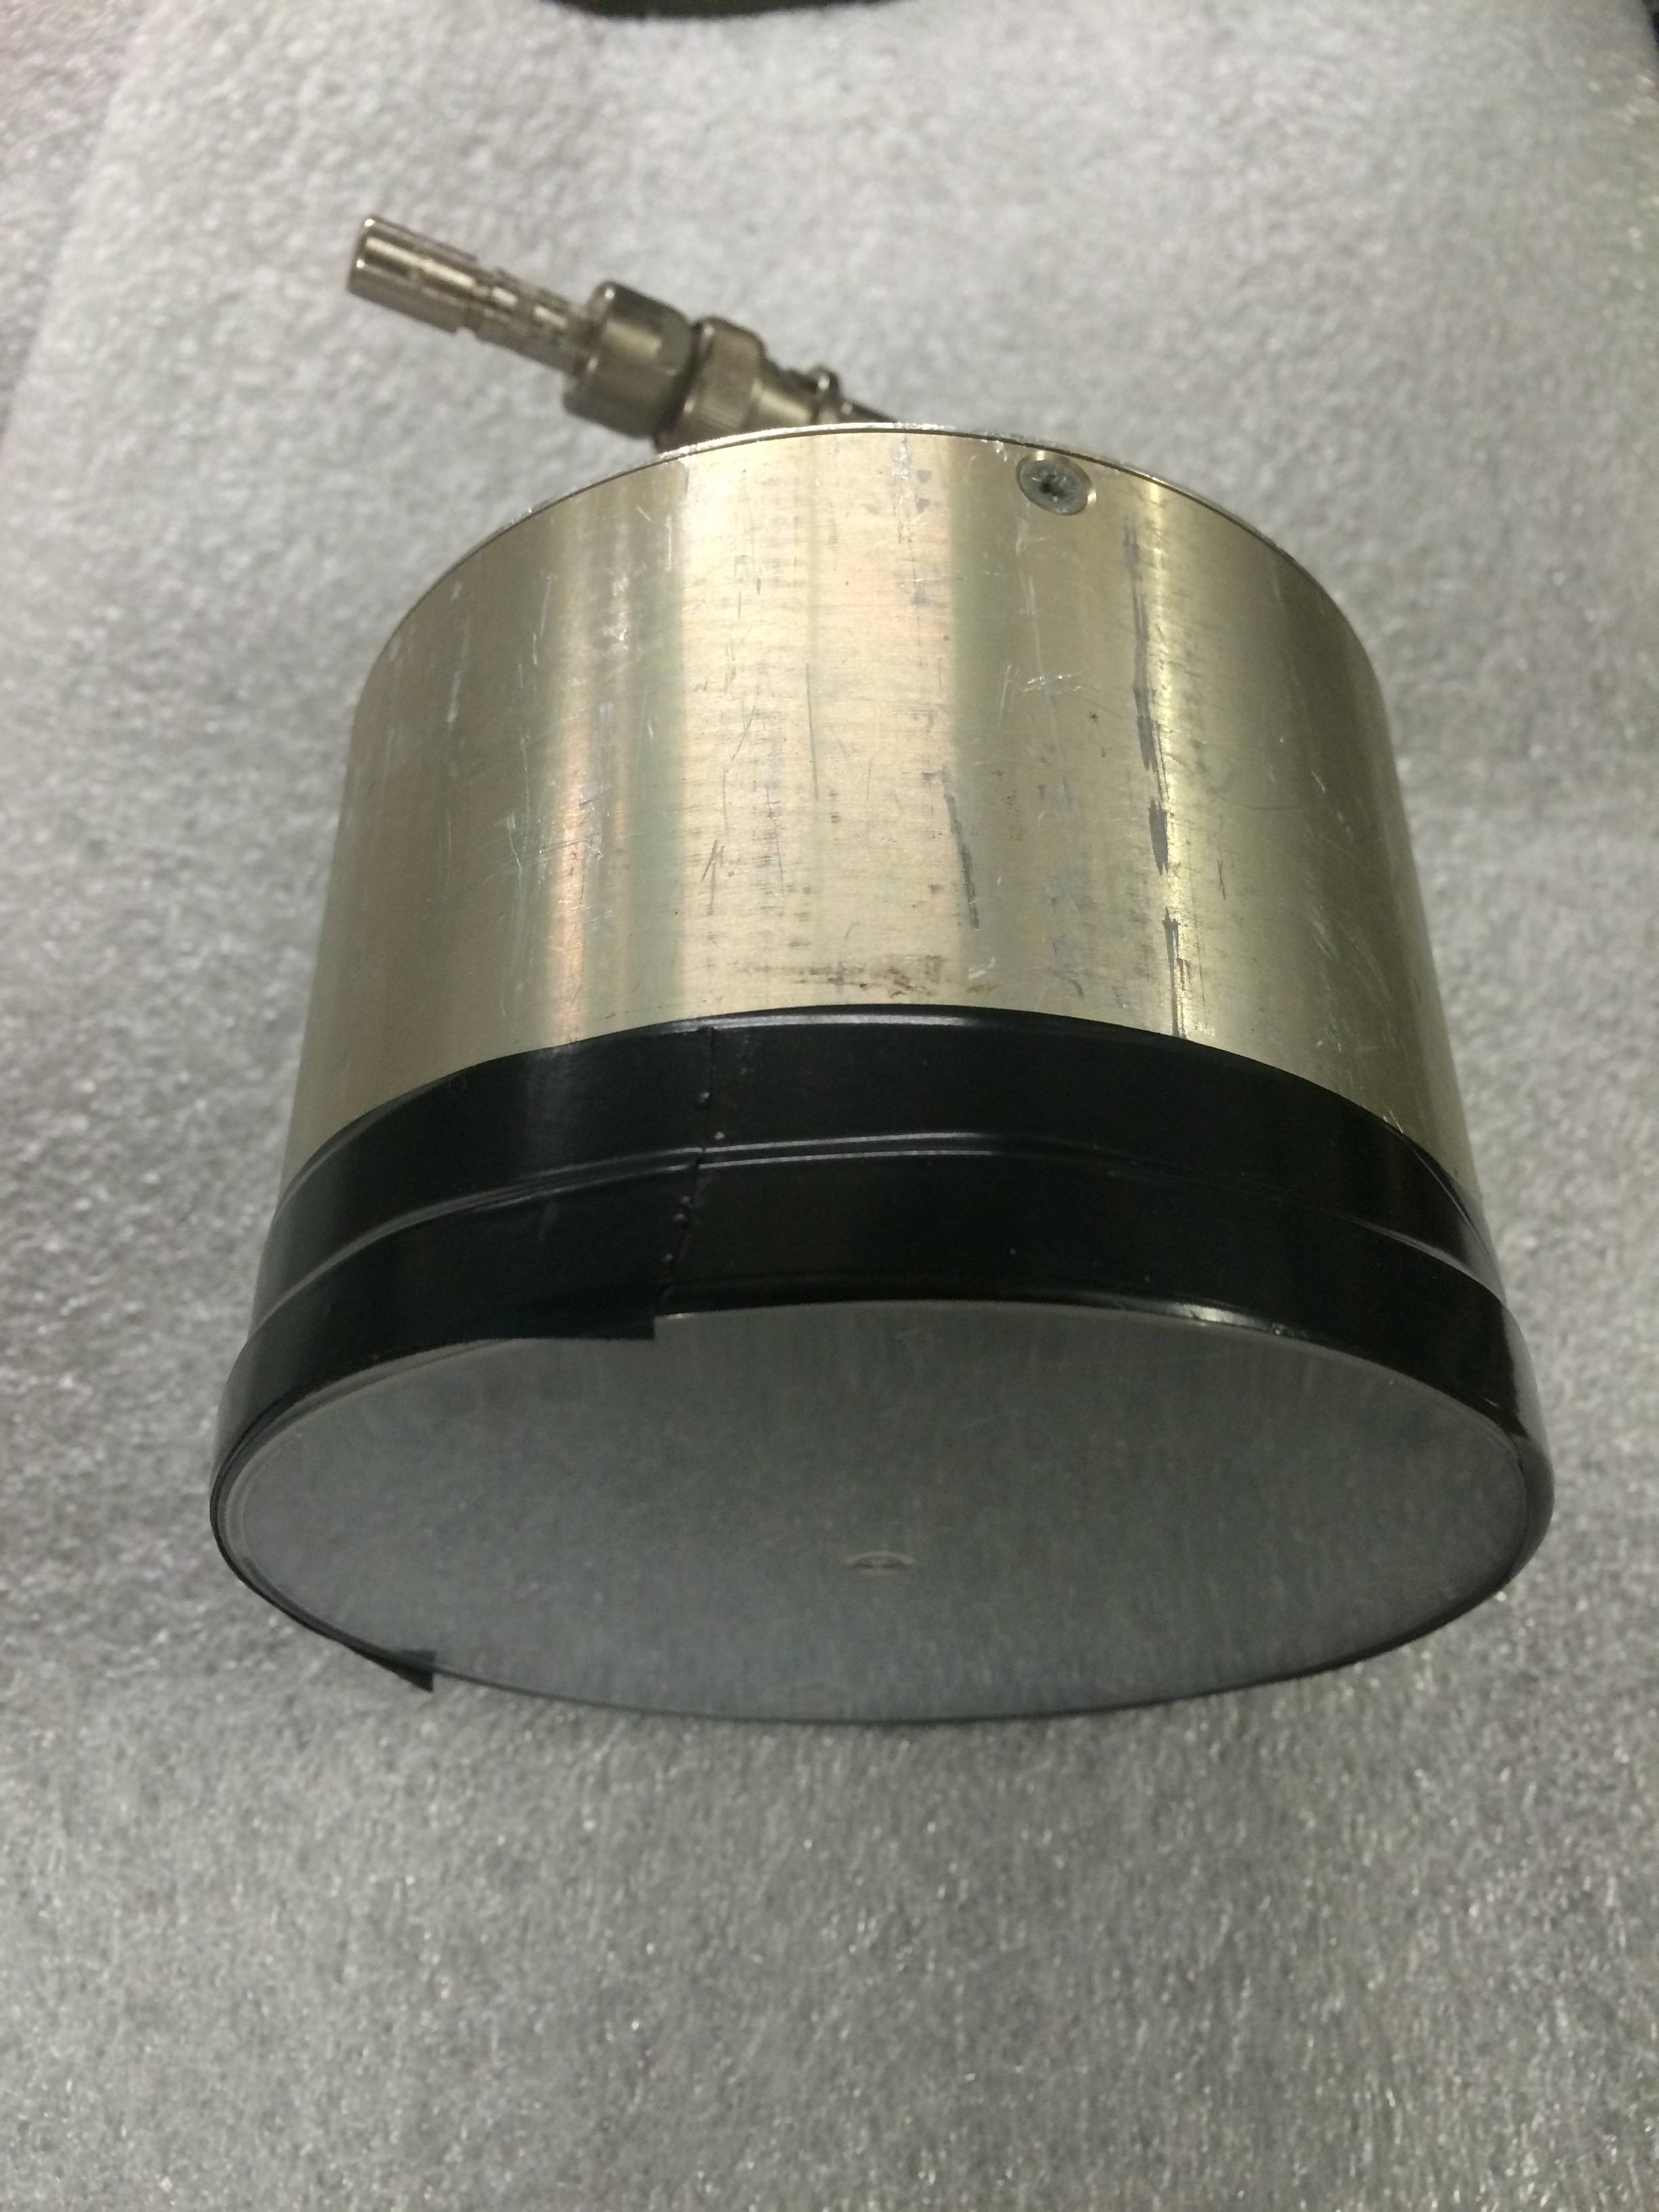
\includegraphics[width = 0.22\textwidth]{Photek}} 
\subfigure[Pico-sil detector, showing the electronic components of the detector. Photo by Javier Duarte.]{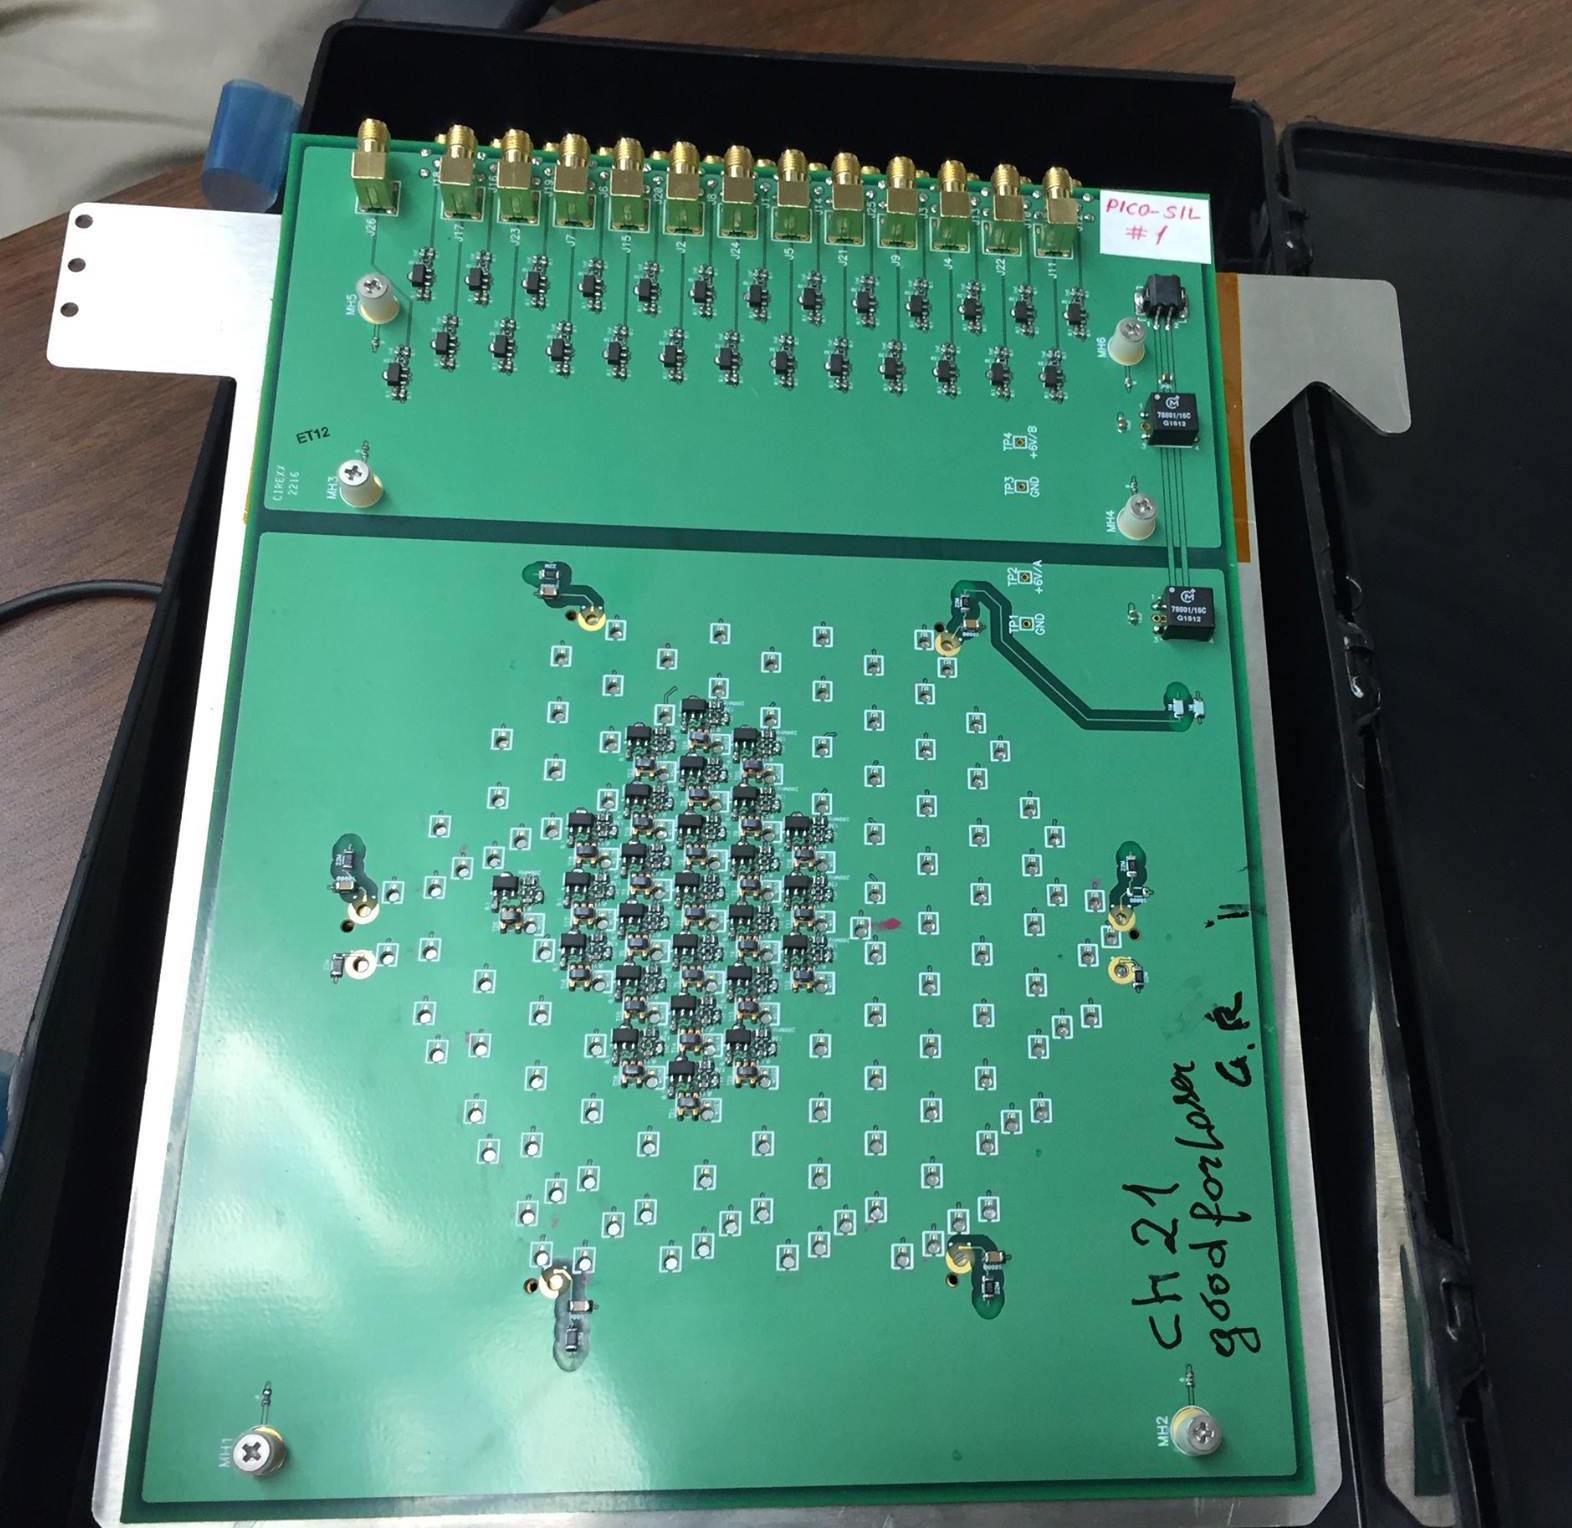
\includegraphics[width = 0.3\textwidth]{picosil}} 
\caption{Pictures of the five detectors used in the test beam. All detectors had black coverings on the front to eliminate any background light seen.}
\label{detectors}
\end{figure*}

Five detectors were used in the test beam runs: pico-sil, silicon pad, Photonis (single channel), Photonis MCP-PMT (64 channel microchannel plate photo multiplier), and a Photek detector (reference timer), with a trigger in front [Figures \ref{detectors} and \ref{beam line}]. The trigger is used to determine when events are seen, essentially as a logic check for the system. All detectors were aligned with the center of the test beam, and the entire detector set up was placed on a cart for alignment with the beam [Figure \ref{beam line}]. A DRS4 was used as the electronic readout for the detectors since it is optimized for intrinsic time resolution studies.

\begin{figure*}[!htbp]
\centering
\subfigure[Set up of the detectors for the beam line test. The pico-sil detector was placed at the very front, just behind the scintillator trigger.]{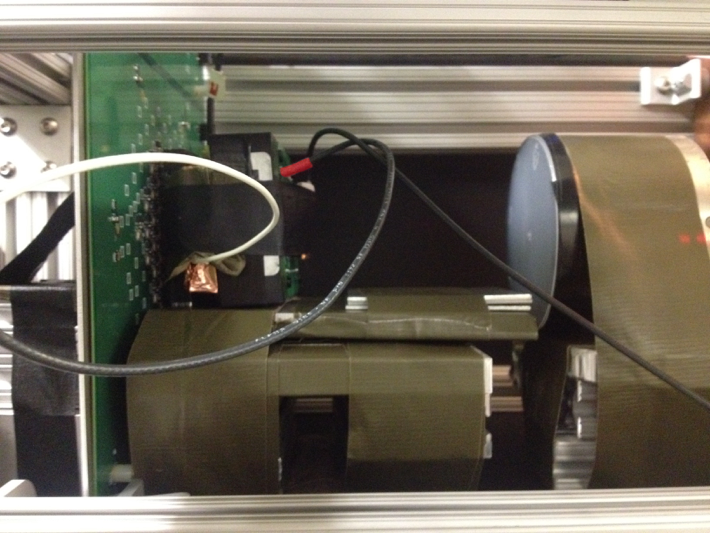
\includegraphics[width = 0.35\textwidth]{whole_set_up}} 
\hspace{8mm}
\subfigure[The cart that was used to align the detectors with the beamline.]{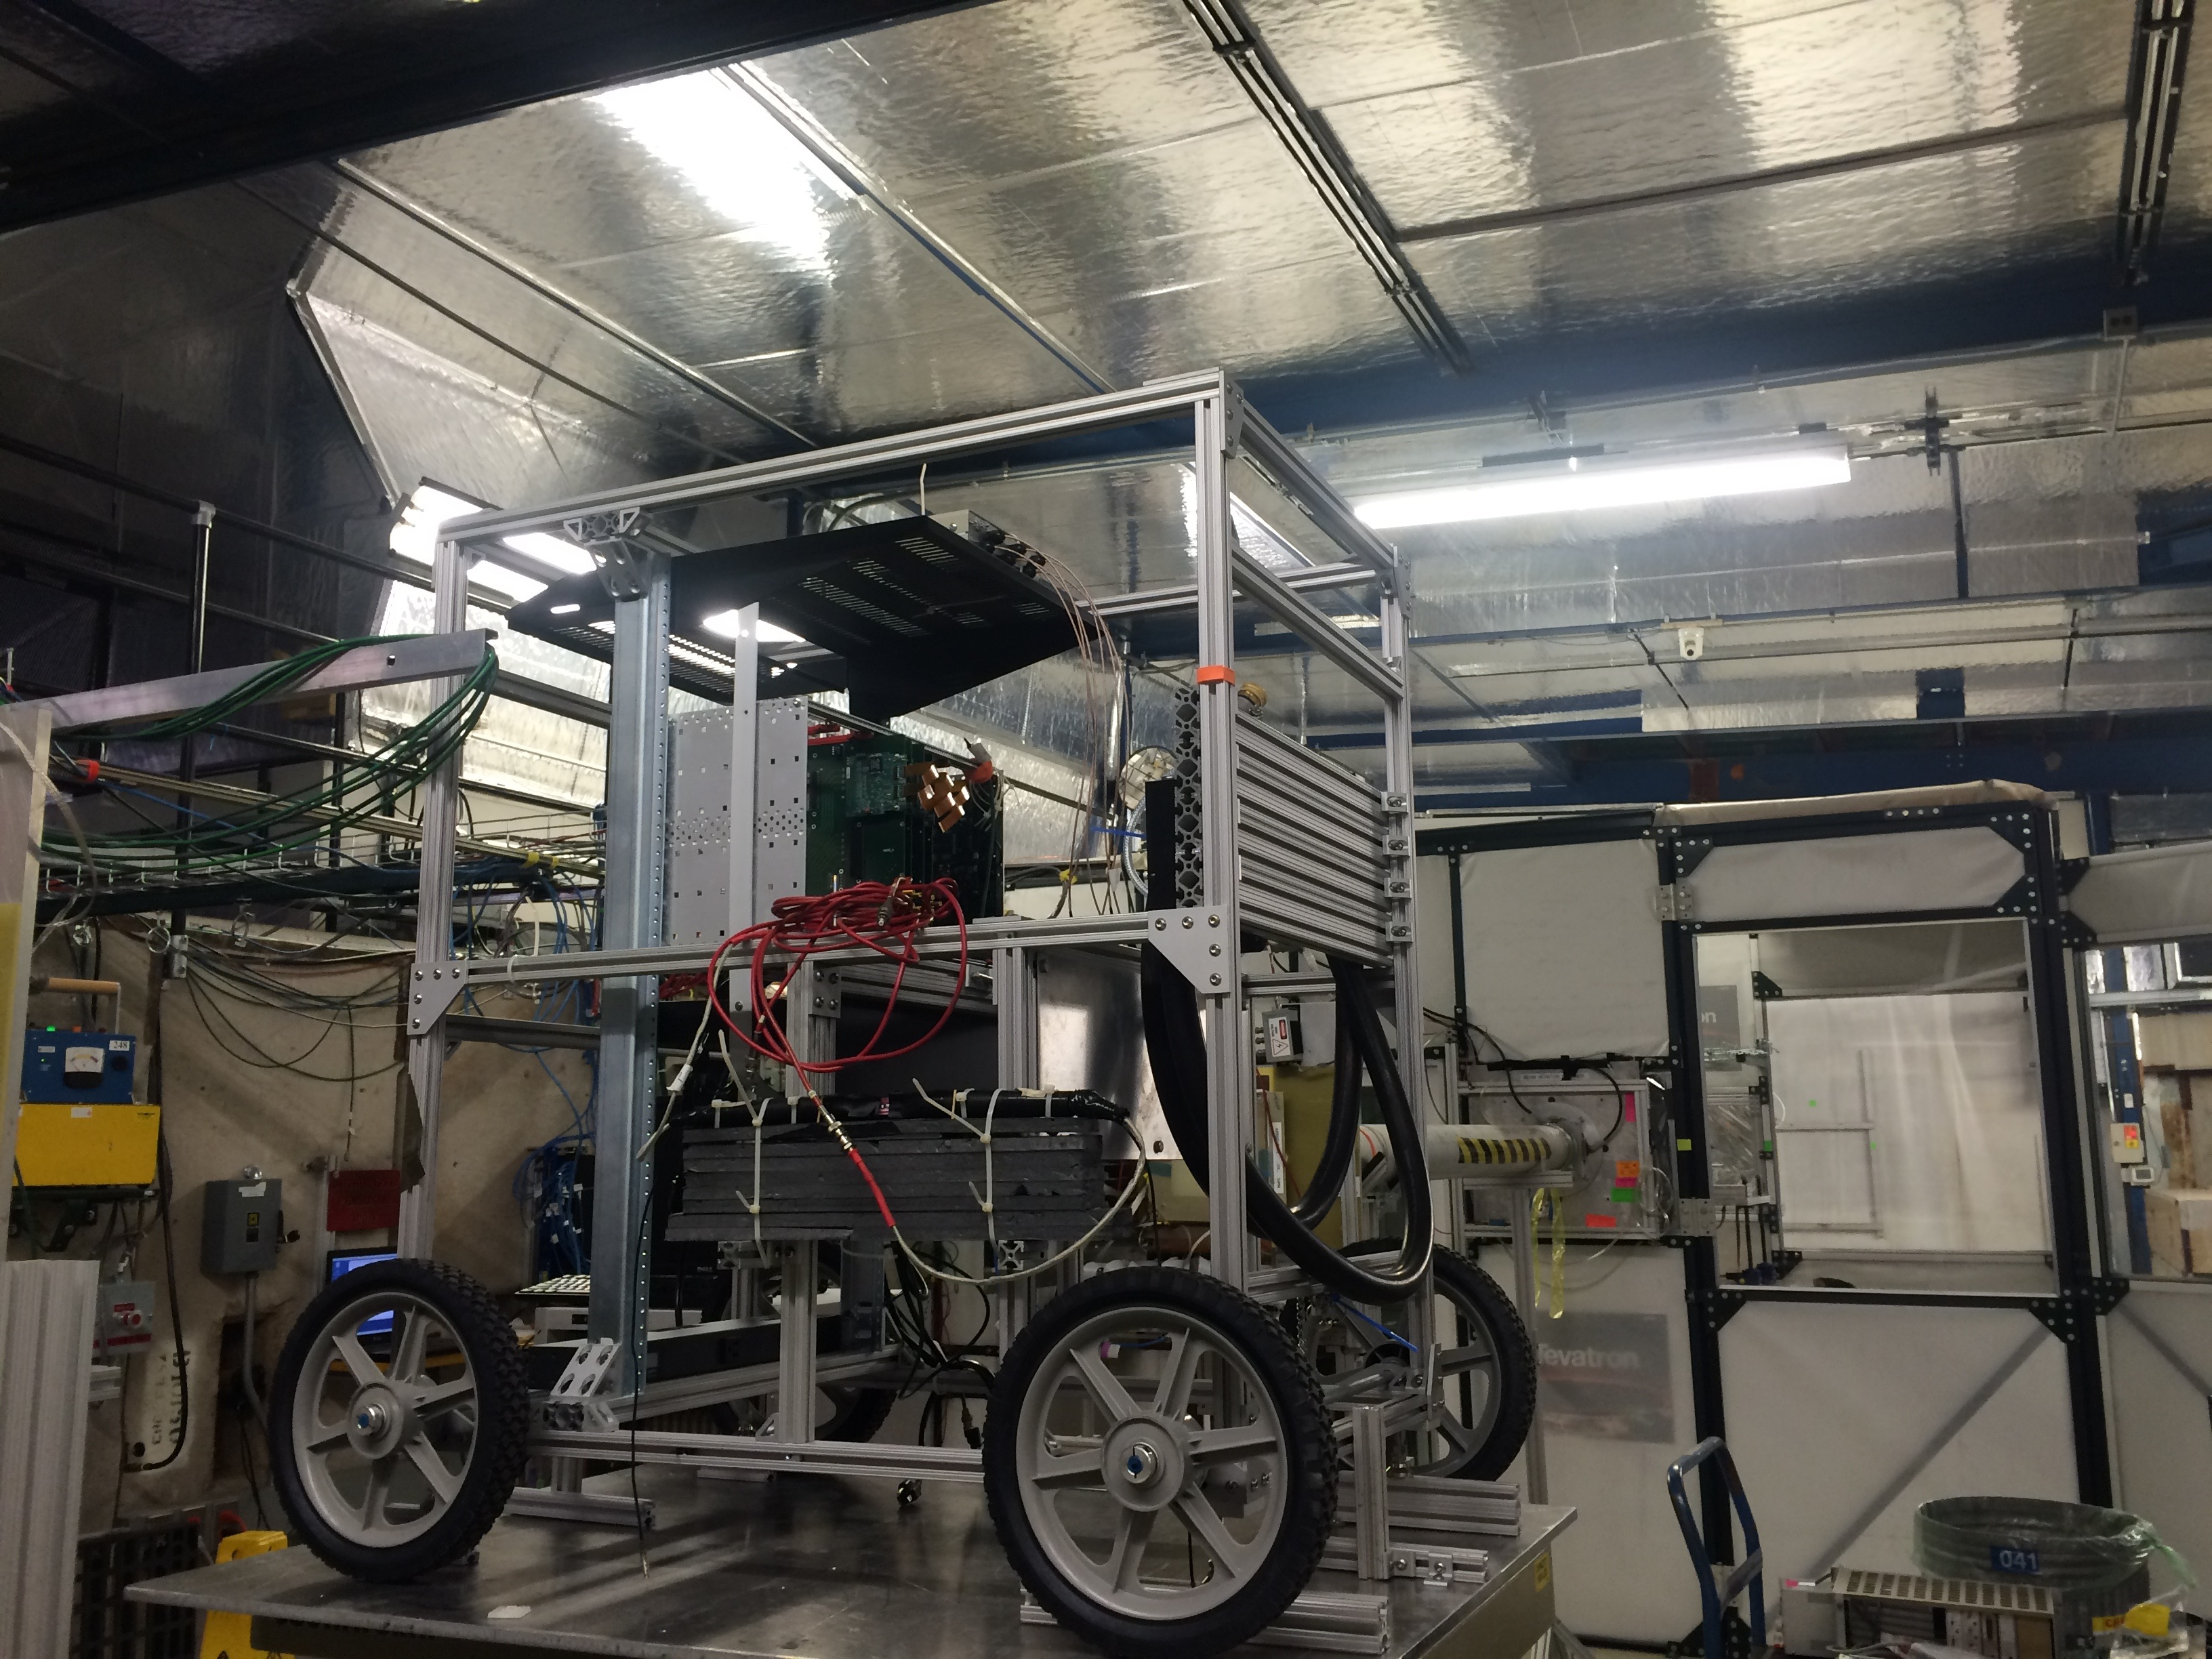
\includegraphics[width = 0.35\textwidth]{cart}}
\subfigure[Diagram of the beamline and the detector alignment. This depicts the main set up used for the runs in this analysis. In some other runs, an absorber was also placed behind the pico-sil HGC.]{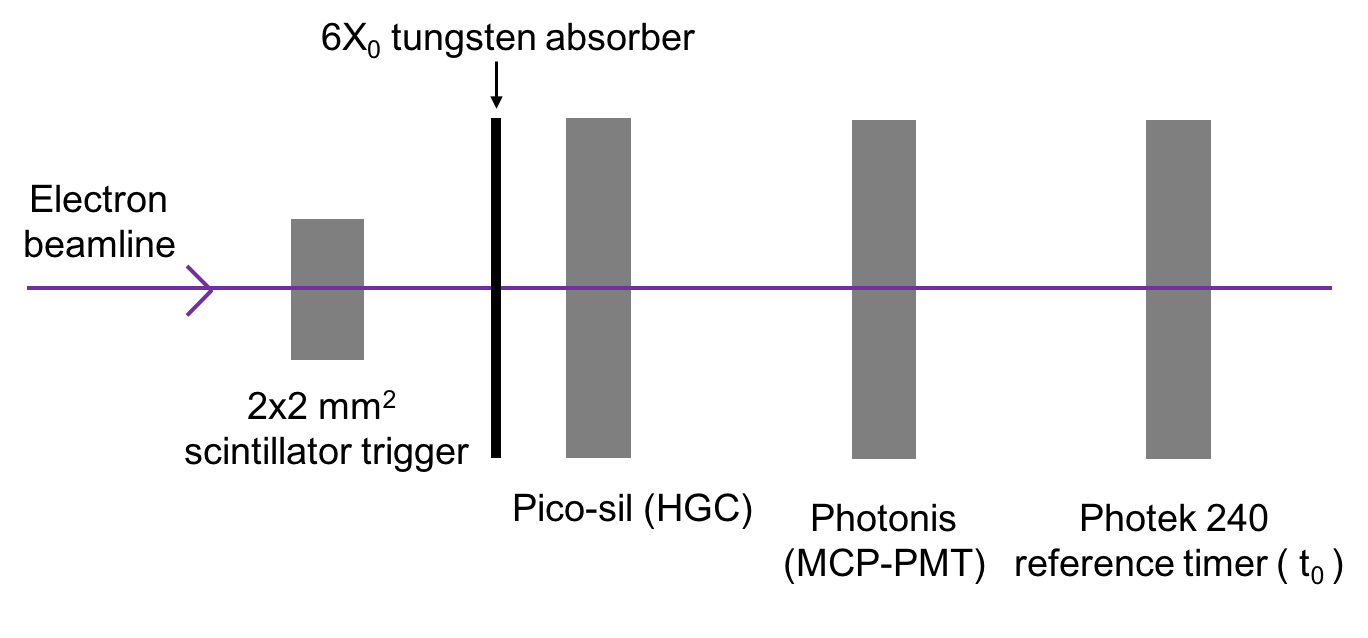
\includegraphics[width = 0.7\textwidth]{detector_diagram}}
\caption{Photo of the detector alignment, cart set up, and a diagram of the detectors, trigger, and absorber in the beamline test.}
\label{beam line}
\end{figure*}

Tungsten or lead absorbers were placed in front of the detectors [Figure \ref{beam line}c], and the distance between the detectors and the absorbers was varied throughout the test beam run. All of this analysis is from runs using a 6 $X_0$ (6 radiation lengths) tungsten absorber placed in front of the pico-sil detector. When the electron beam hits the absorber, a shower of electrons and photons is created, and is then observed by the detectors.  The electromagnetic shower is created through Bremsstrahlung and pair production. Bremsstrahlung occurs when an electron approaches a nucleus and the electron loses kinetic energy, electromagnetic radiation is produced, and the electron is converted to a photon and a lower energy electron. The Bremsstrahlung cross section is proportional to $Z^2$ ($Z$ is the atomic number of the nucleus) \cite{Leo}. Pair production is when a photon is converted to an electron-positron pair, where momentum is conserved by a nearby nucleus. The pair production cross section is also proportional to $Z^2$ \cite{Leo}.

Since each detector is at a different spatial position in the shower, each observes a different portion of the shower. Additionally, when the distance between the pico-sil detector and the absorber is varied, the pico-sil observes the shower at a wider or more narrow point - which can be quantified by observing the transverse spread of the shower. The pico-sil detector is made of multiple pixels, arranged in a hexagonal tiling [Figure \ref{pico-sil}]. Each pixel is recorded independently, so the transverse spread of the shower is recorded. The integral (integral of the current vs. time plot for an event, giving units of electric charge, and proportional to the total energy observed by the pixel) of each of the pixels on the pico-sil detector was calculated and plotted for various positions of the tungsten absorber and electron beam energies [Figure \ref{integral tungsten distance}]. Thus, these plots show the total energy observed by each pixel.

\begin{figure*}[!htbp]
\centering
\subfigure[$6X_0$ tungsten absorber placed 1 mm from the pico-sil detector, with 32 GeV electron beam]{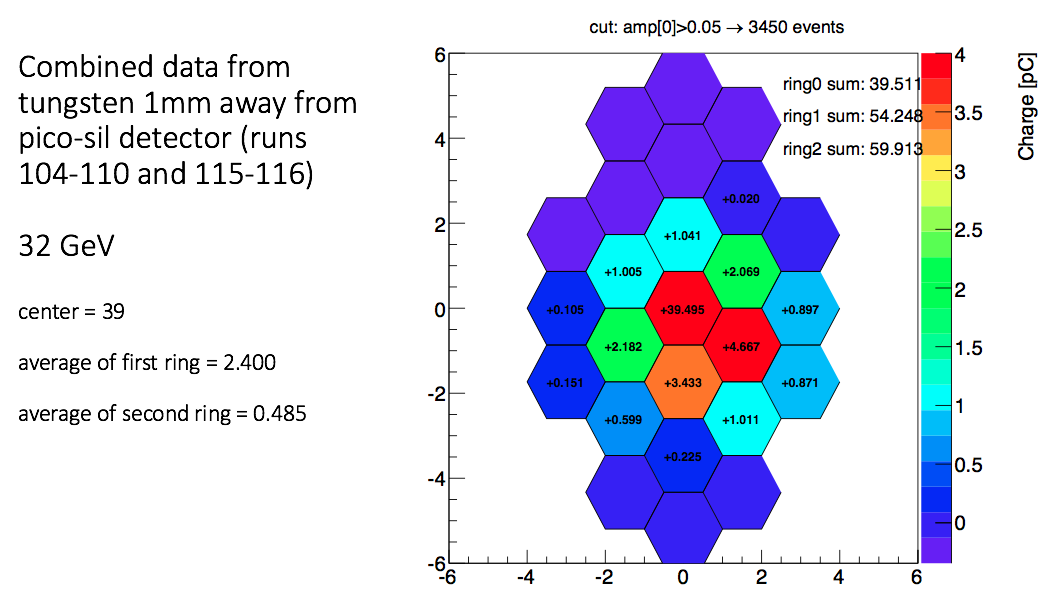
\includegraphics[width = 0.45\textwidth]{tungsten_1mm_32}} 
\subfigure[$6X_0$ tungsten absorber placed 1 cm from the pico-sil detector, with 32 GeV electron beam]{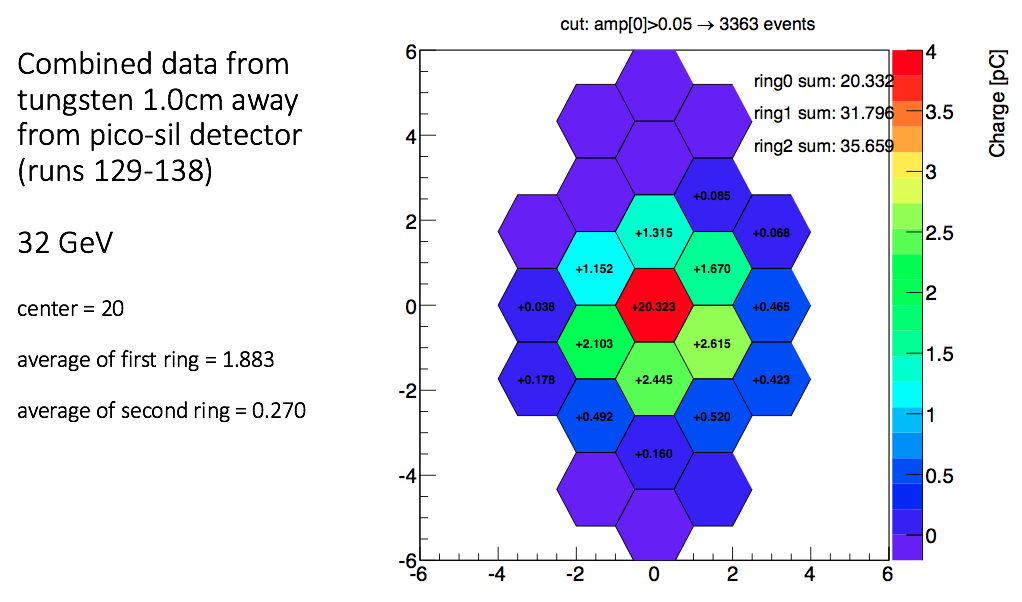
\includegraphics[width = 0.45\textwidth]{tungsten_1cm_32}}
\subfigure[$6X_0$ tungsten absorber placed 3.2 cm from the pico-sil detector, with 32 GeV electron beam]{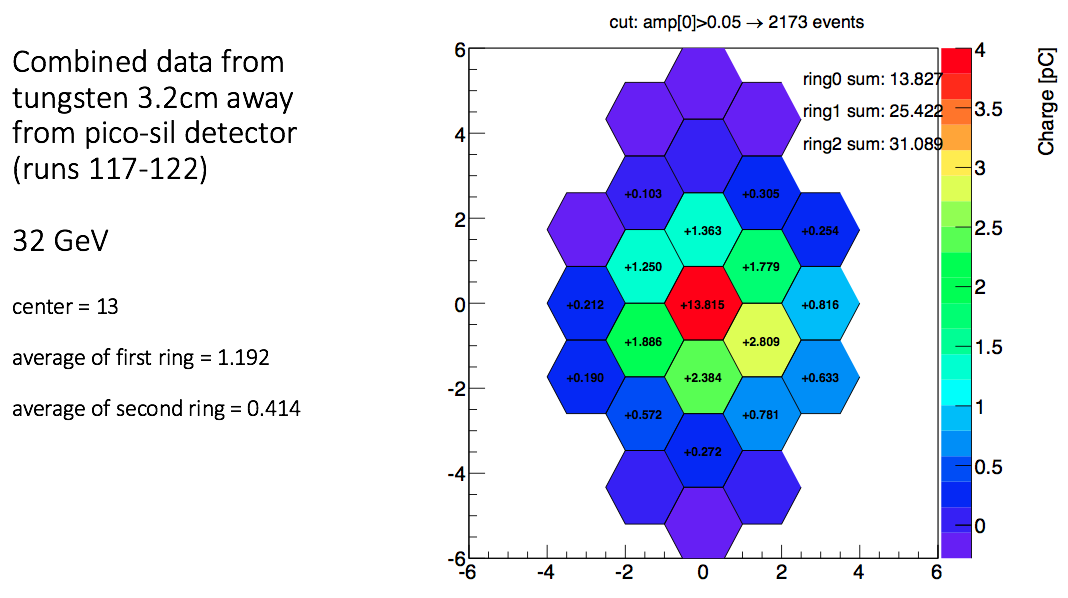
\includegraphics[width = 0.45\textwidth]{tungsten_3cm_32}}
\subfigure[$6X_0$ tungsten absorber placed 7.5 cm from the pico-sil detector, with 32 GeV electron beam]{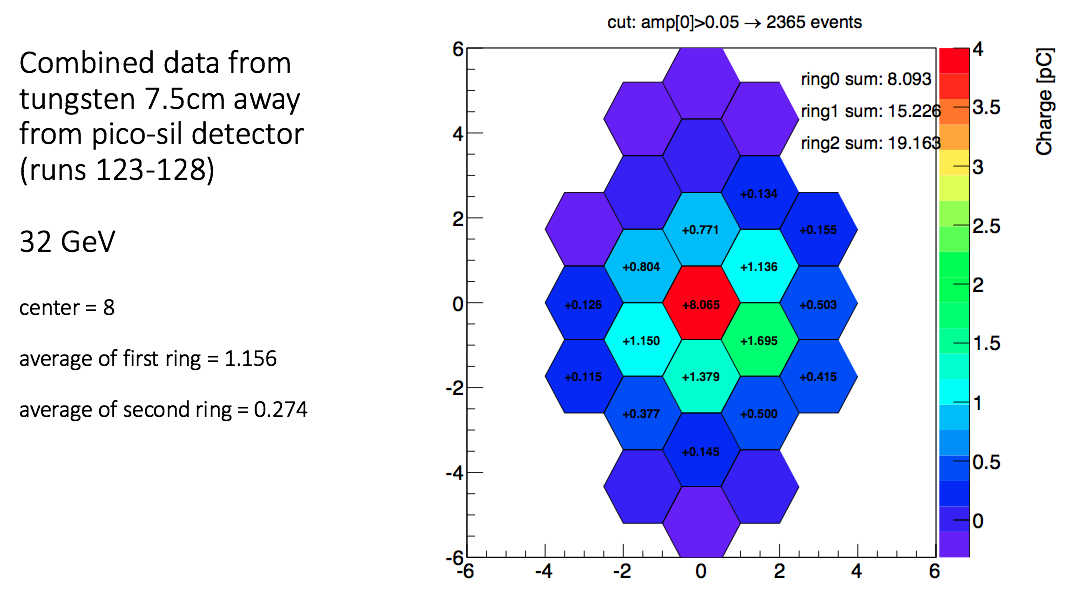
\includegraphics[width = 0.45\textwidth]{tungsten_7cm_32}} 
\caption{Plots of the integral for each pixel on the pico-sil detector, with the absorber at varying distances from the detector. The integral is proportional to the total energy observed by the detector, and it is seen that as the tungsten is moved further away from the pico-sil, less energy is observed.}
\label{integral tungsten distance}
\end{figure*}

\begin{figure}[!htbp]
\subfigure[$6X_0$ tungsten absorber placed 1 mm from the pico-sil detector, with 32 GeV electron beam]{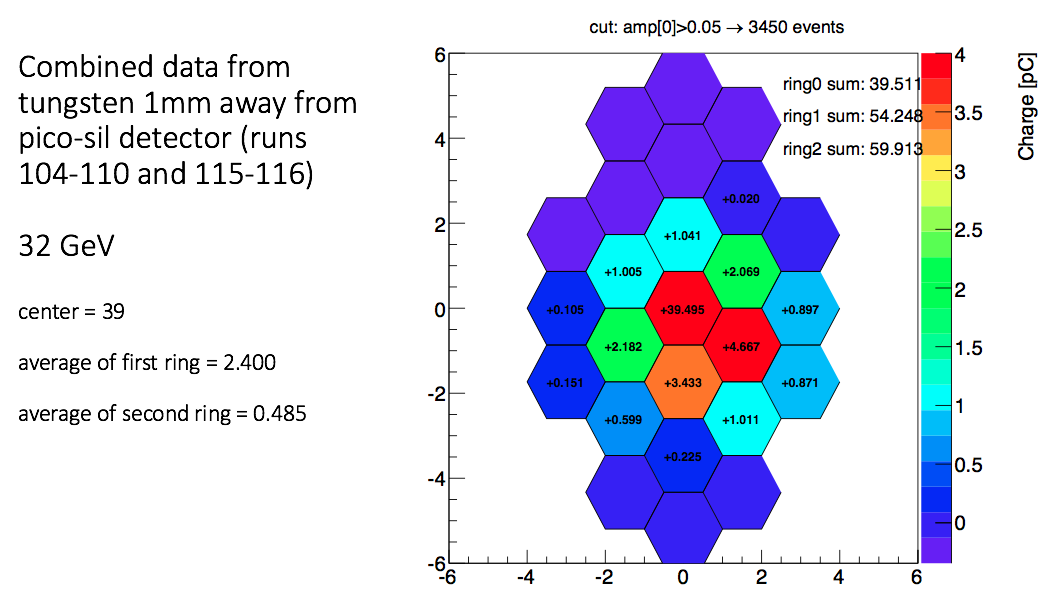
\includegraphics[width = 2in]{tungsten_1mm_32}} 
\subfigure[$6X_0$ tungsten absorber placed 1 mm from the pico-sil detector, with 16 GeV electron beam]{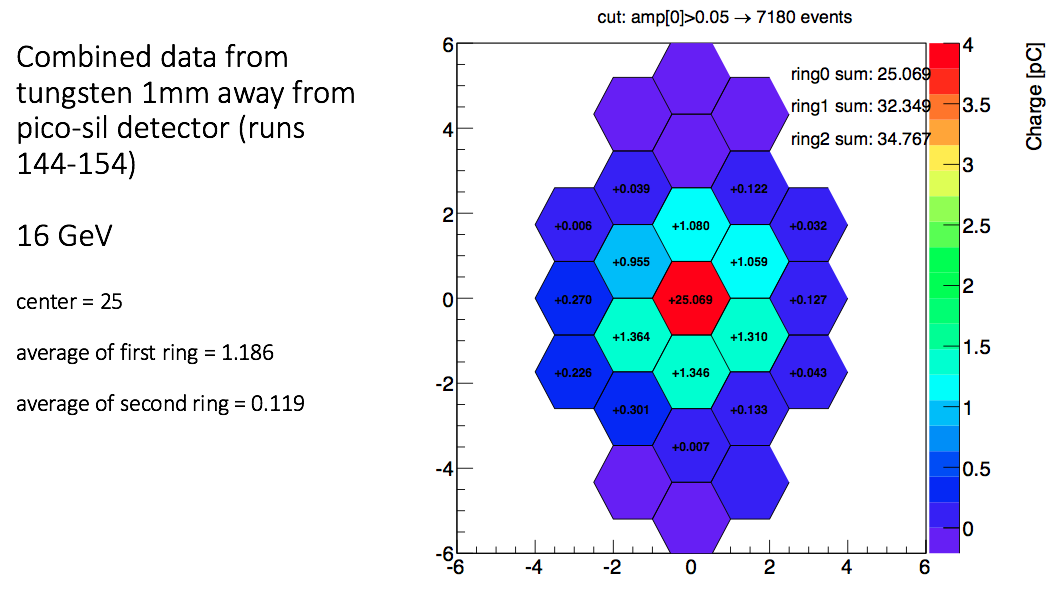
\includegraphics[width = 2in]{tungsten_1mm_16}}
\caption{Plots of the integral for each pixel on the pico-sil detector, with the absorber 1 mm from the detector, and with an electron beam of 32 and 16 GeV. The integral is proportional to the total energy observed by the detector, and it is seen that with the 16 GeV electron beam, about half of the energy is observed, as expected.}
\label{integral tungsten energy}
\end{figure}

When the tungsten absorber is further away from the pico-sil detector, less total energy is seen by the detector [Figure \ref{integral tungsten distance}]. This is seen by the decrease in the ``ring2 sum'' as the distance between the detector and absorber is increased. However, the amount of energy seen by the pixels further from the center (in the first or second ring) does not increase significantly, but remains constant or decreases. This is not expected - we expected the further away pixels to see an increased amount of energy as the detector is further from the absorber, since they are seeing a later part of the shower. However, it is seen that the energy is concentrated in the center pixel for all distances. Additionally, when the energy contained is plotted for 32 and 16 GeV electrons with the tungsten at 1 mm, it is seen that the beam is focused on the center pixel, and the first ring has about half of the energy for the 16 GeV beam as compared to the 32 GeV beam, as expected [Figure \ref{integral tungsten energy}]. These plots give the typical beam spread for the various beam energies and absorber distances.

Additionally, the spread in the shower can be seen by plotting the ratio of the charge observed by the central pixel to the charge observed by all pixels. As the $6X_0$ tungsten absorber is moved further away from the pico-sil, the ring pixels contain more of the total charge per event on average. The ratio between the charge contained in the central pixel and all pixels is plotted in Figure \ref{charge ratios}.

\begin{figure}[!htbp]
{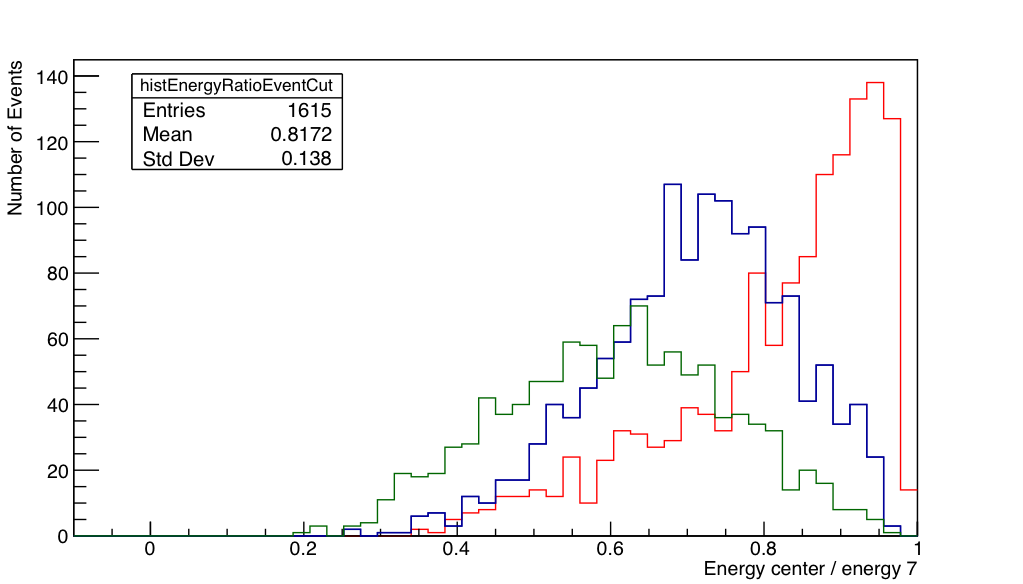
\includegraphics[width = .5\textwidth]{center_all_ratio}} 
\caption{Histogram of the number of events vs ratio of the charge contained in the central pixel to all pixels. 1 mm is shown in red, 10 mm in blue, and 32 mm in green. 75 mm is not plotted, but overlaps 32 mm significantly.}
\label{charge ratios}
\end{figure}

\section{Data Analysis and Results}

This analysis focuses on analyzing the effects of combining information from the pico-sil transverse pixels on the determined time resolution.

The Photek detector is used as the reference timer for all analysis, as it has an outstanding time resolution of 10 ps (measured in previous test beam analyses). The time difference of the detection of an event between the pico-sil and the Photek is due to the distance between the two - which is expected to be a Gaussian. The absolute difference in time (the mean of the Gaussian) does not matter, but rather the standard deviation ($\sigma$) gives the time resolution since this is the spread in the time difference between the two measurements of the event.

In an event, a ``pulse'' is recorded by each detector, and by the individual pixels in the pico-sil. The Photek (reference timer) has a Gaussian response to an event, and thus its timestamp is determined as the mean of the Gaussian fit to the pulse. The pico-sil pixels do not have a Gaussian response (the rise time is shorter than the fall time), and thus a linear fit is used on the rising edge from 10\% to 90\% of the maximum amplitude values. The timestamp of the pixel is determined by the time when the linear fit is at 45\% of the maximum amplitude. Examples of the timestamp fits are shown in Figure \ref{timestamp}.

\begin{figure}[!htbp]
\subfigure[Fit of the pulse observed in the Photek to a Gaussian, with the mean of the Gaussian indicated.]{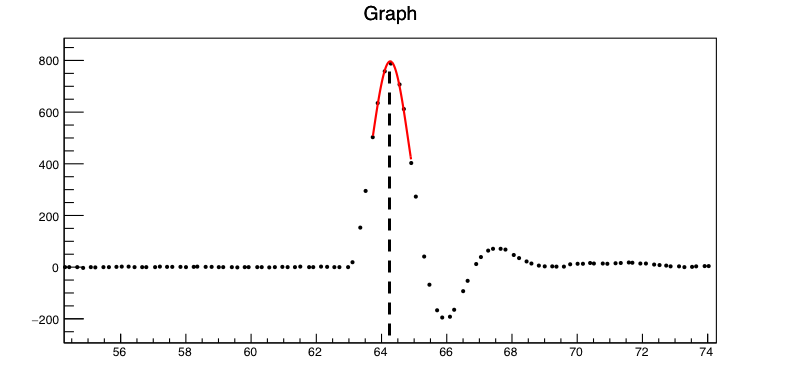
\includegraphics[width = 0.5\textwidth]{photek_gaussian}} 
\subfigure[Linear fit of the rising edge of the pico-sil pixel response, with the 45\% maximum amplitude point indicated.]{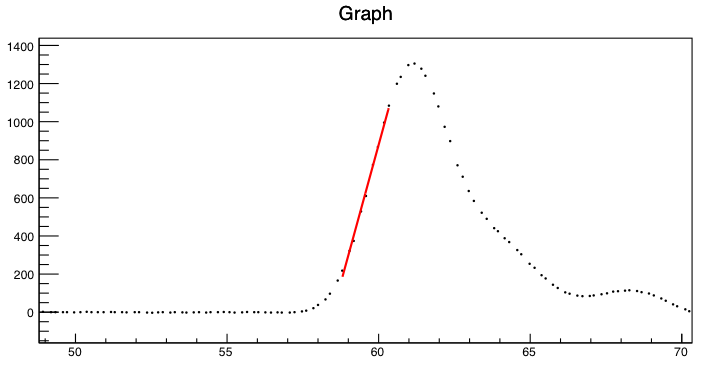
\includegraphics[width = 0.45\textwidth]{pixel_linear_fit}}
\caption{Pulses observed in the pico-sil HGC detector and the Photek with the fits to determine the timestamp shown. The fits for the Photek pulse and the pico-sil pixel pulse are a Gaussian and linear fit, respectively.}
\label{timestamp}
\end{figure}

Many events are recorded, however, not all events are from the electron beam. Thus, electron events must be separated from the background events (pions and muons primarily). The background events have a much lower charge than the electron events, and thus charge and amplitude cuts on the central pixel and the Photek are used to select electron events. Events are selected based on observing signal both in the Photek and in the center pixel of the pico-sil, since this is where the electron beam is focused. Histograms of events vs. event charge are shown in Figure \ref{charge amp cuts}, with the cuts indicated. Electron events are the Gaussian to the right of the cut, while the background events are centered around 0 pC. Charge and amplitude cuts for the Photek and the central pixel vary based on the beam energy and absorber distance from the pico-sil, and the cuts are shown in Table \ref{table:cuts}.

\begin{figure}[!htbp]
\subfigure[Histogram of number of events vs. Photek charge, with the cut indicated by the black line.]{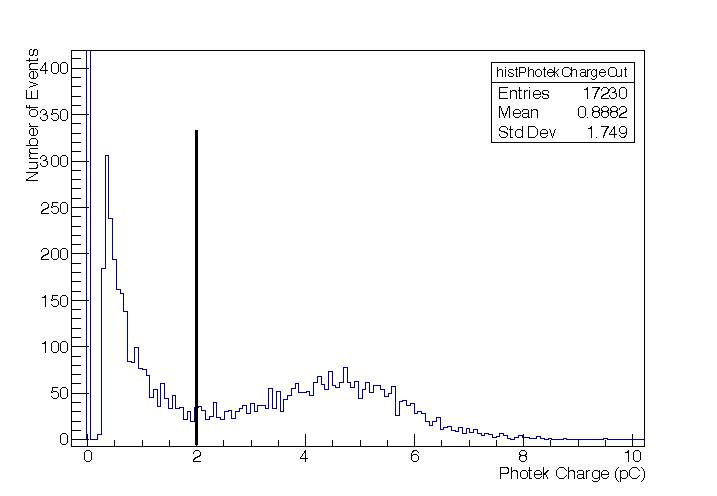
\includegraphics[width = 0.5\textwidth]{Photek_Charge}} 
\subfigure[Histogram of number of events vs. Photek amplitude, with the cut indicated by the black line.]{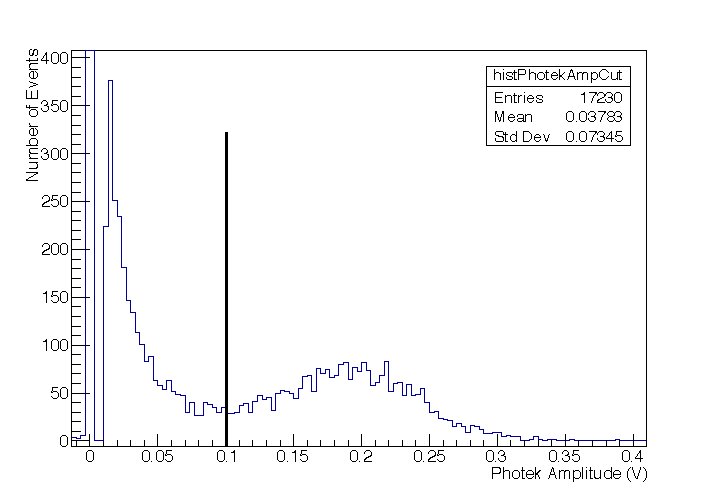
\includegraphics[width = 0.5\textwidth]{Photek_Amp}}
\caption{Histograms and cuts indicated for the charge and amplitude cuts on the Photek to select electron events. These plots are from the 32 GeV $6X_0$ tungsten 1mm away from the pico-sil runs.}
\label{charge amp cuts}
\end{figure}

When multiple pixels are added to determine the time resolution from their combined information, each pixel used in the combination must pass both charge and amplitude cuts (charge $>$ 1 pC and amplitude $>$ 0.01 V). Time information from each pixel is either added with equal weighting, or with weighting based on the magnitude of charge the pixel contains. If a pixel does not pass these cuts, it is added with a weighting of 0, such that the event can still be used even if not every pixel passes the cuts. This means that when all pixels are combined, in most events, actually 3 or 4 pixels are combined, since it is rare for all 7 pixels to pass the cuts within the same event. Plots of the number of pixels passing the cuts per event are shown in Figure \ref{pixels average}.

\begin{centering}
\begin{table*}[!htbp]
  \begin{tabular}{ | c | c | c | c | c | c | c | }
    \hline
    \multirow{2}{*}{Run} & Beam Energy & Separation & Photek amp & Photek charge & Center amp & Center charge \\
 & (GeV) & Distance (mm) & cut (V) & cut (pC) & cut (V) & cut (pC) \\ \hline
    104-110, 115, 116 & 32 & 1 & 0.1 & 2 & 0.15 & 11 \\ \hline
    129-138 & 32 & 10 & 0.1 & 2 & 0.1 & 8 \\ \hline
    117-122 & 32 & 32 & 0.09 & 2 & 0.05 & 3 \\	\hline
    123-128 & 32 & 75 & 0.09 & 2 & 0.03 & 2 \\ \hline
    144-155 & 16 & 1 & 0.03 & 0.8 & 0.01 & 2.5 \\ \hline
	167-171 & 8 & 1 & 0.015 & 0.4 & 0.01 & 2.5 \\ \hline
	46-52 & 8 & 32 & 0.04 & 1 & 0.01 & 1 \\ \hline
  \end{tabular}
\caption[Table caption text]{Table of charge and amplitude cuts for the center and Photek to select electron events.}
\label{table:cuts}
\end{table*}
\end{centering}

\subsection{Time Resolution with Pico-sil Detector Pixel Combination}

When the central pixel from the pico-sil is analyzed with the Photek detector acting as the reference timer, the time resolution is around 16 ps [Figure \ref{pixel TOF 1mm}a]. For each event, the seven pico-sil pixels are ordered by how much energy they observe, and then combined in this order. It is expected that as more pixels are combined, the time resolution will improve, as the amount of time information about the event is increased. When the pixels are added together to determine the time resolution, they are added in order of how much energy they observed (starting with the pixel with the most energy), and their time measurements are either weighted by energy contained in the pixel, or equally for every pixel.

To measure the time resolution improvement, the time resolution of the center pixel alone is compared to the time resolution of all 7 closest pixels (central plus the first ring of 6 pixels, Figure \ref{pico-sil}). The time resolution is determined by fitting the $\Delta$t vs. number of events histogram to a Gaussian, using the range $\pm$2 RMS around the mean of the histogram [Figure \ref{pixel TOF 1mm}]. All fits were done with the log-likelihood method, as this is a better statistical method for bins with low numbers of events (as many of the histograms have approaching the tails).

\begin{figure*}[!htbp]
\subfigure[The time resolution fit for the central pixel only.]{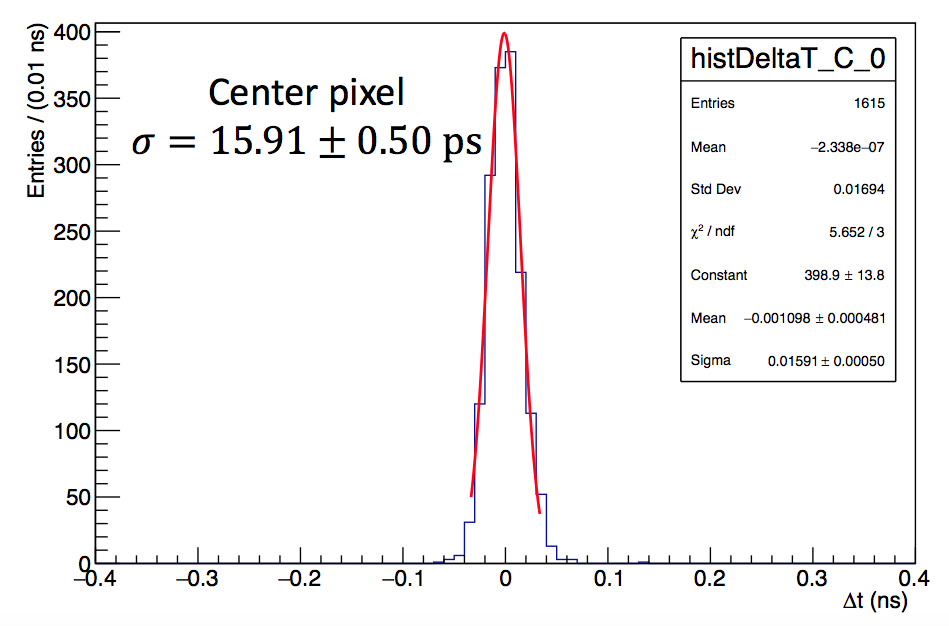
\includegraphics[width = 0.3\textwidth]{32_1mm_central}} 
\subfigure[The time resolution fit for all 7 pixels, combined with equal weighting for each pixel.]{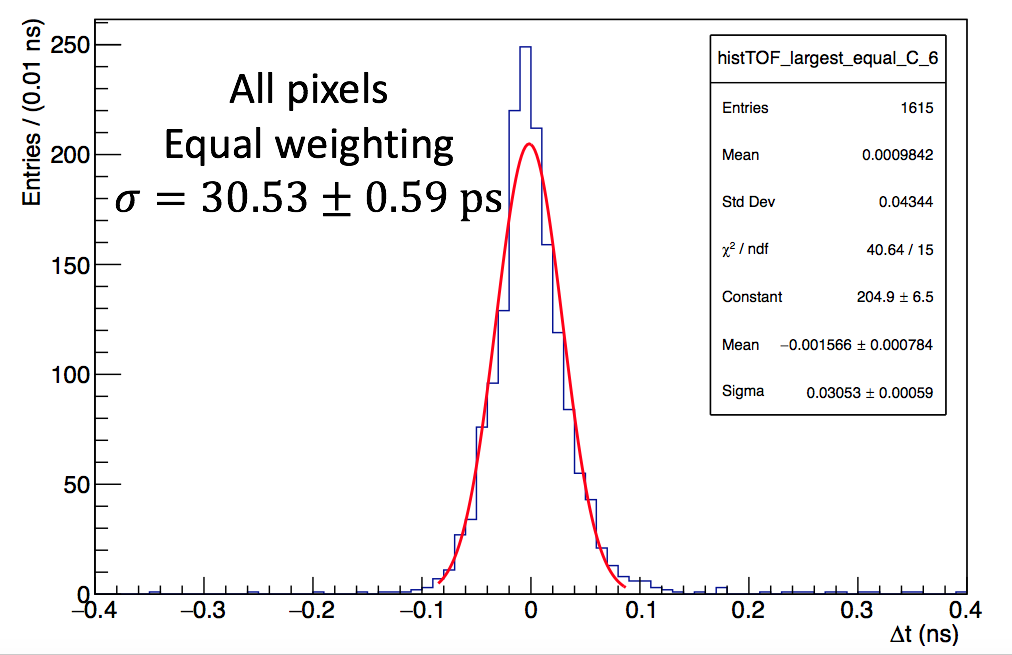
\includegraphics[width = 0.3\textwidth]{32_1mm_equal}} 
\hspace{3mm}
\subfigure[The time resolution fit for all 7 pixels, combined with weighting based on the charge contained in each pixel.]{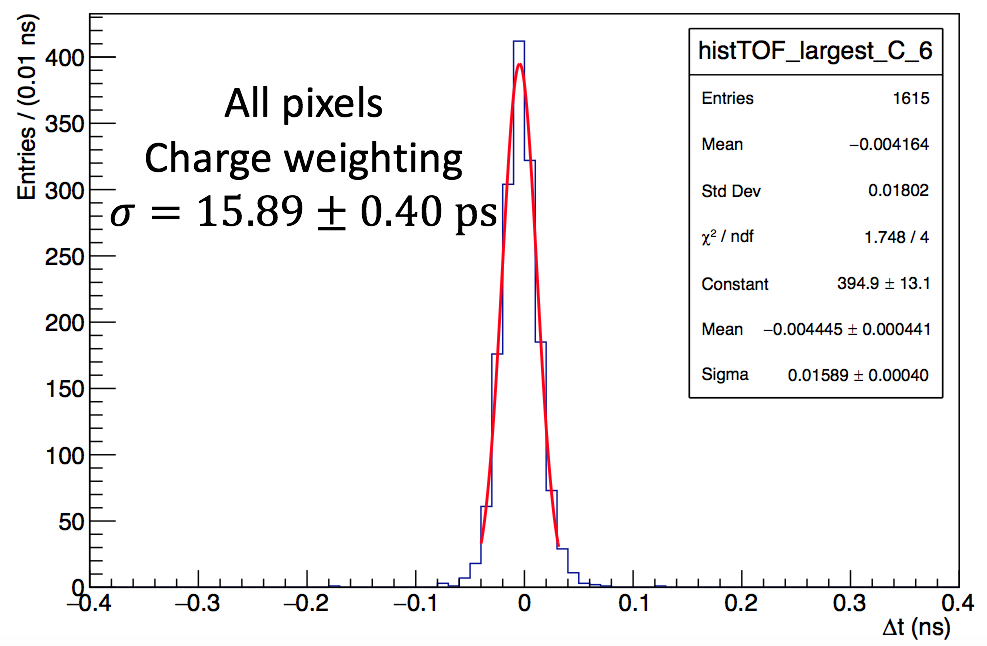
\includegraphics[width = 0.3\textwidth]{32_1mm_charge}} 
\hspace{3mm}
\caption{Time resolution plots for the 32 GeV electron data, with the tungsten absorber at 1mm from the pico-sil absorber. When all 7 pixels are combined equally, the time resolution is made worse than just the central pixel time resolution alone, and when the pixels are combined by charge weighting, the time resolution remains approximately the same.}
\label{pixel TOF 1mm}
\end{figure*}

The analysis of the time resolution with 1mm separation between the absorber and pico-sil with a 32 GeV electron beam show that an outstanding time resolution of under 16ps has been measured [Figure \ref{pixel TOF 1mm}].

It was found that combining the pixels with equal weighting does not improve the time resolution, but rather makes it considerably worse [Figure \ref{resolution charge equal}]. This is due to the individual time resolutions of the ring pixels (around 60 ps) being considerably worse than that of the central pixel (15.9 ps), and thus an equal weighting gives a worse time resolution than the central pixel alone. Charge weighting the time information did not improve the time resolution either [Figure \ref{resolution charge equal}]. This is likely because most of the time information was already contained in the central pixel, so by adding additional pixels, significant information is not added.

The same analysis was done with the 6$X_0$ tungsten absorber at 10mm, 32mm, and 75mm from the pico-sil detector, and the results are shown in Figure \ref{resolution charge equal}. In all cases, combining pixels by equal weighting makes the time resolution worse, while charge weighting keeps the time resolution approximately the same as the resolution for the center pixel alone. Additionally, there was no significant improvement in the shape of the histograms or their tails seen when the pixels are combined by charge weighting - indicating that combining pixels does not provide an advantage over determining time resolution from the center pixel alone for these arrangements. If the shower were more spread and the first ring pixels had a larger signal, there may be an improvement in the time resolution seen by combining pixels, since in this case the additional pixels would be adding more time information. Further tests with a larger shower spread would be needed to confirm this.

\begin{figure*}[!htbp]
\centering
\subfigure[Plot of the time resolutions for the central pixel and all 7 pixels combined (for tungsten at various distances from the pico-sil absorber). The combination is done with equal pixel weighting.]{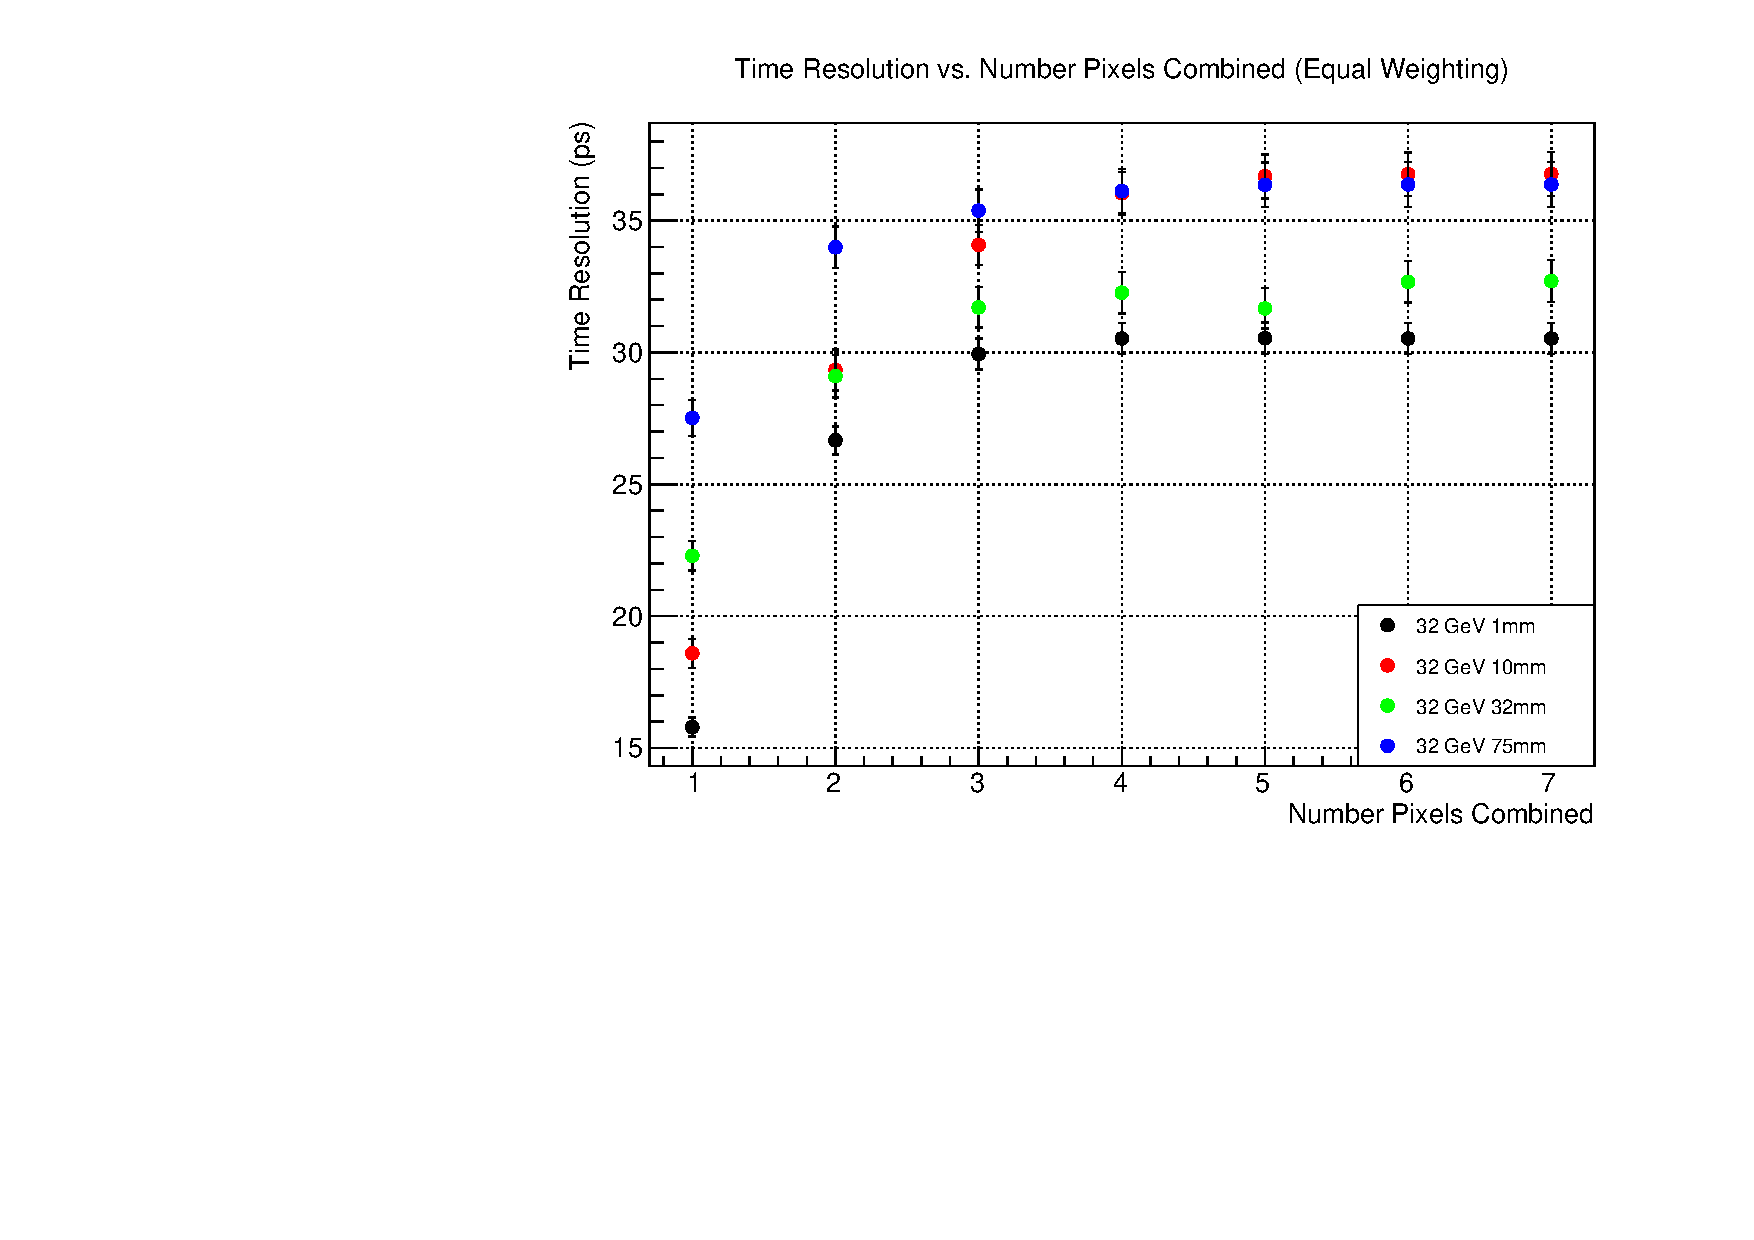
\includegraphics[width = .49\textwidth]{equal_weighting}} 
\subfigure[Plot of the time resolutions for the central pixel and all 7 pixels combined (for tungsten at various distances from the pico-sil absorber). The combination is done with pixel weighting based on the charge contained in the pixels.]{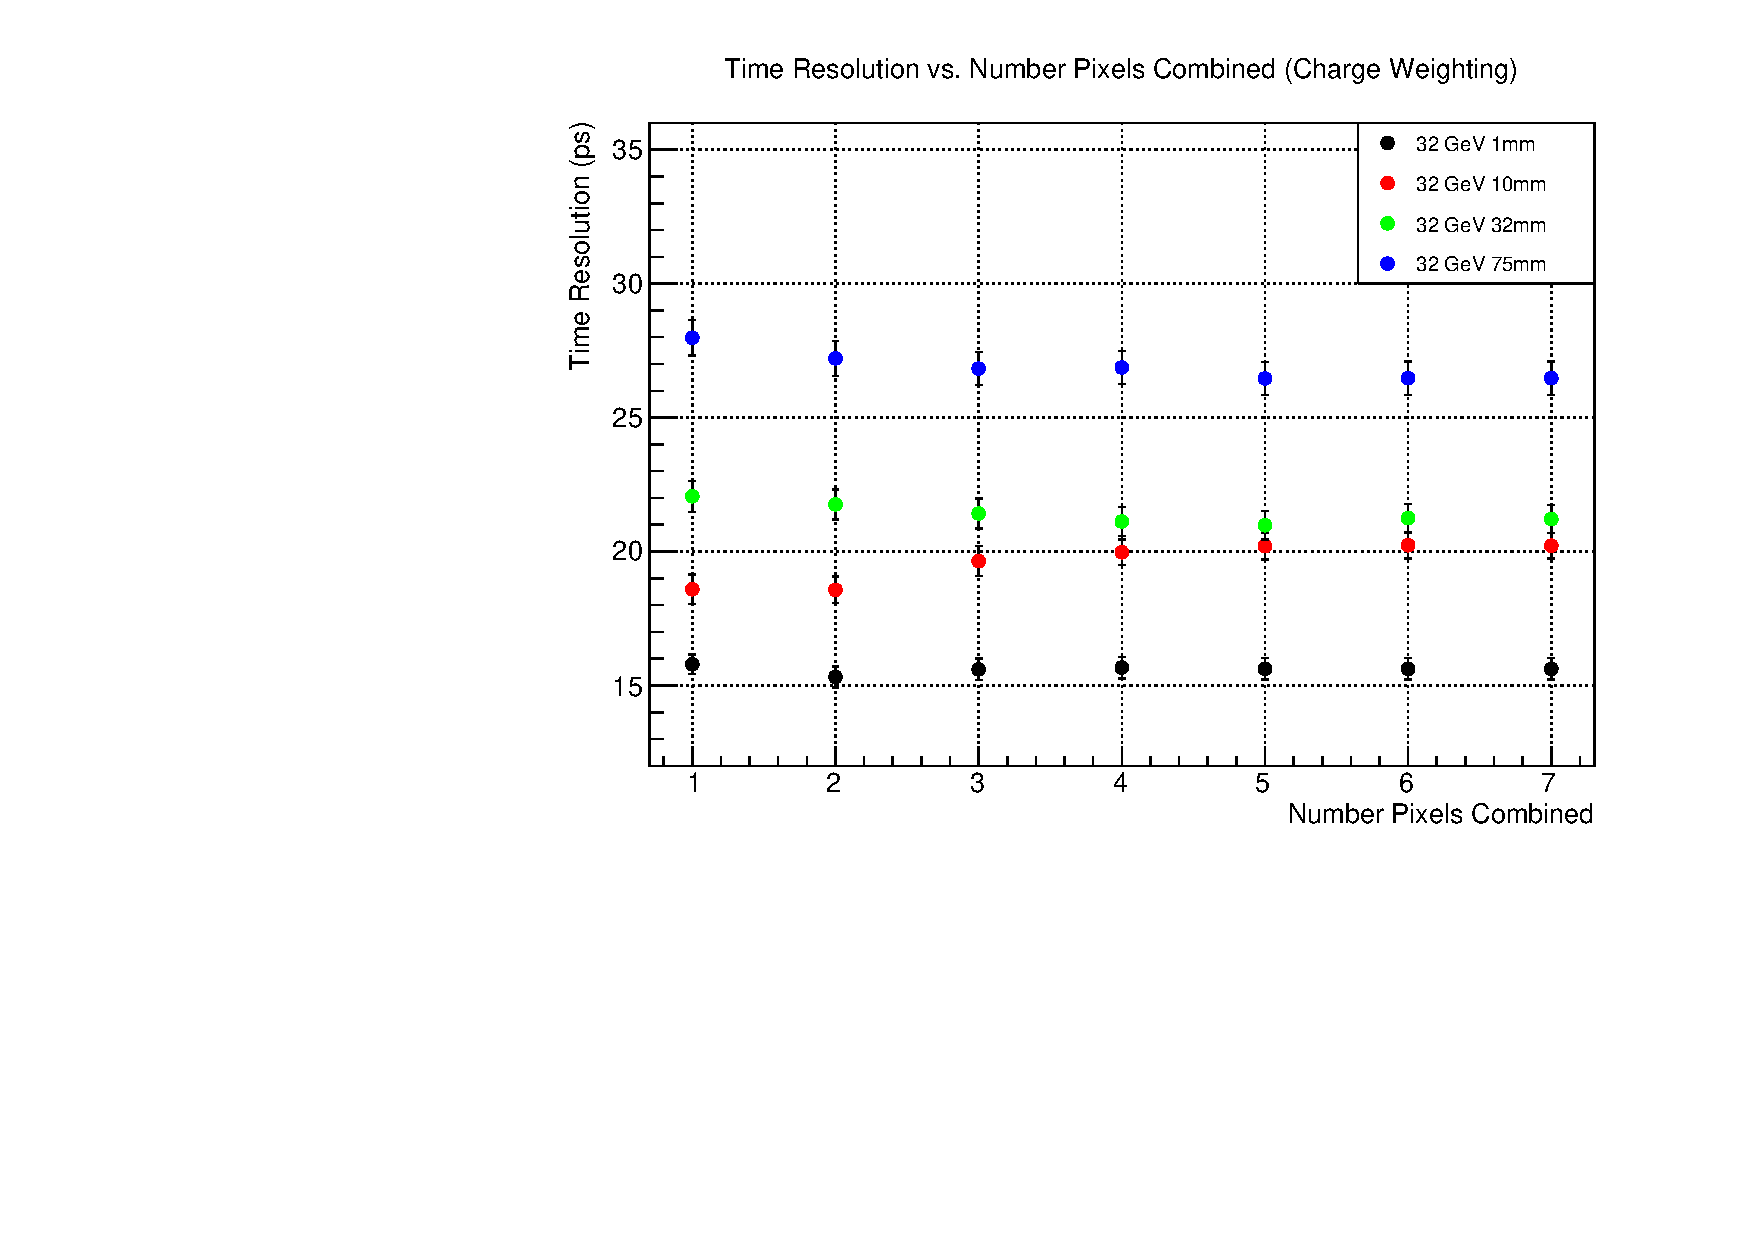
\includegraphics[width = .49\textwidth]{charge_weighting}} 
\caption{The time resolution (in ps) plotted vs. the number of pixels combined. With equal pixel weighting, the time resolution is made worse by the combination of all 7 pixels, and with charge weighting, the time resolution is approximately the same as with just the central pixel.}
\label{resolution charge equal}
\end{figure*}

\subsection{SKIROC Time Smearing}

In the Phase II Upgrade, the HGC in the CMS detector to replace the CMS wil be read out with an analog to digital conversion chip. A SKIROC2 (Silicon Kalorimeter Integrated ReadOut Chip) chip that converts the analog signals from detector channels to digital signals will be used. There is an intrinsic digital noise added when the SKIROC2 chip is used, as it would be in the actual HGC detector set up \cite{Callier}, and the effect of this chip on the time resolution is investigated. All of the previous analysis has been done without this additional noise consideration.

To determine the effect of the SKIROC2 chip, a time smearing was done to model the noise present in the analog to digital conversion that will be done in the HGC. The SKIROC chip was represented by adding random noise in each pixel by ``smearing'' the determined time resolution in each event by adding a random number generated from a Gaussian distribution with mean 0 and sigma 50ps (since 50ps is the estimated noise from use of the SKIROC2 chip). Smearing was also done with a distribution with sigma 500 ps to determine the effect of larger smearings on the time resolution. The larger smearing is mostly for a confirmation that when pixels have the same beginning time resolution, combining them improves the time resolution following Equation \ref{square root N}. After this is done, the time resolutions for the center pixel and combined 7 pixels (equal and charge weighted) are determined.

\begin{figure*}[!htbp]
\centering
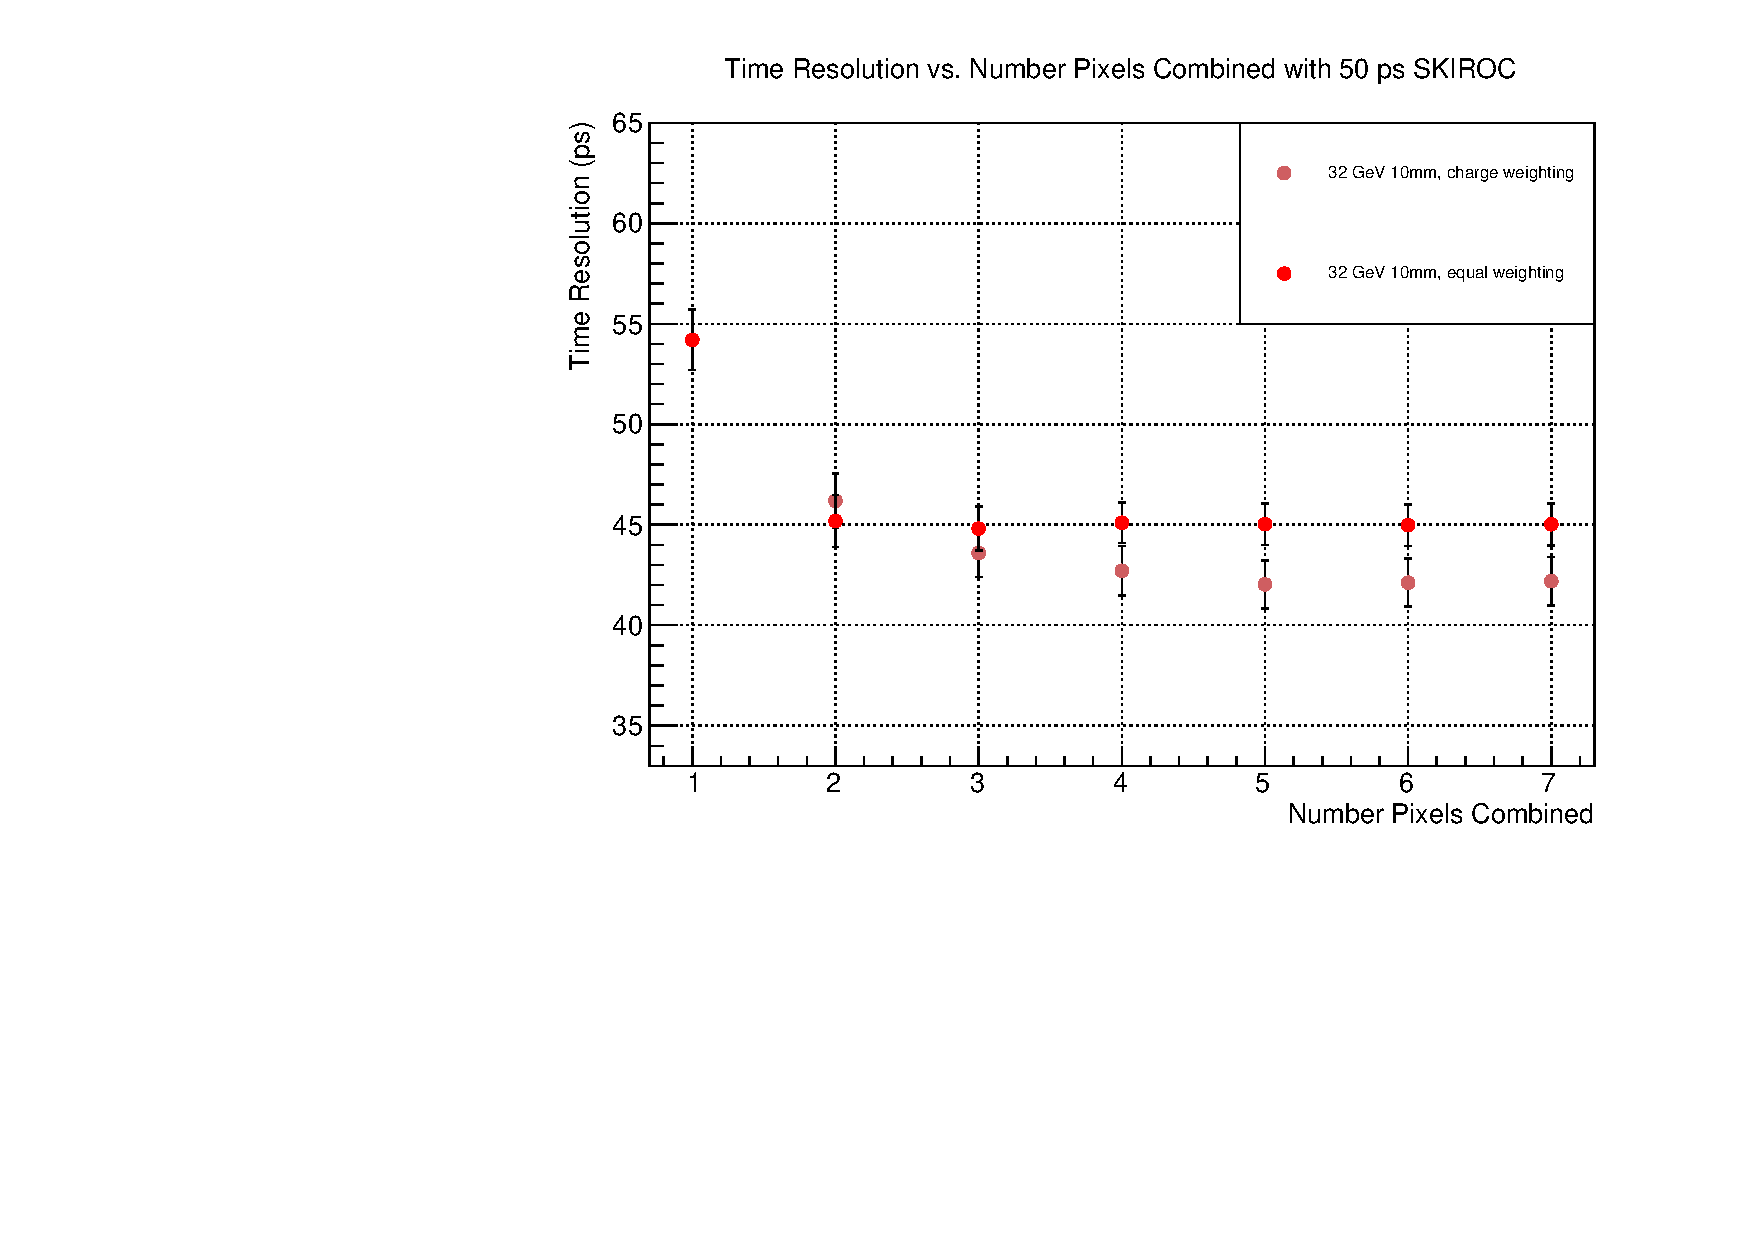
\includegraphics[width = 0.8\textwidth]{smearing_50_10mm}
\caption{Results of the SKIROC smearing analysis with 50 ps smearing. This is for the 10mm separation data, and is representative of the other distances with the 32 GeV electron beam.}
\label{50 smearing}
\end{figure*}

\begin{figure*}[!htbp]
\centering
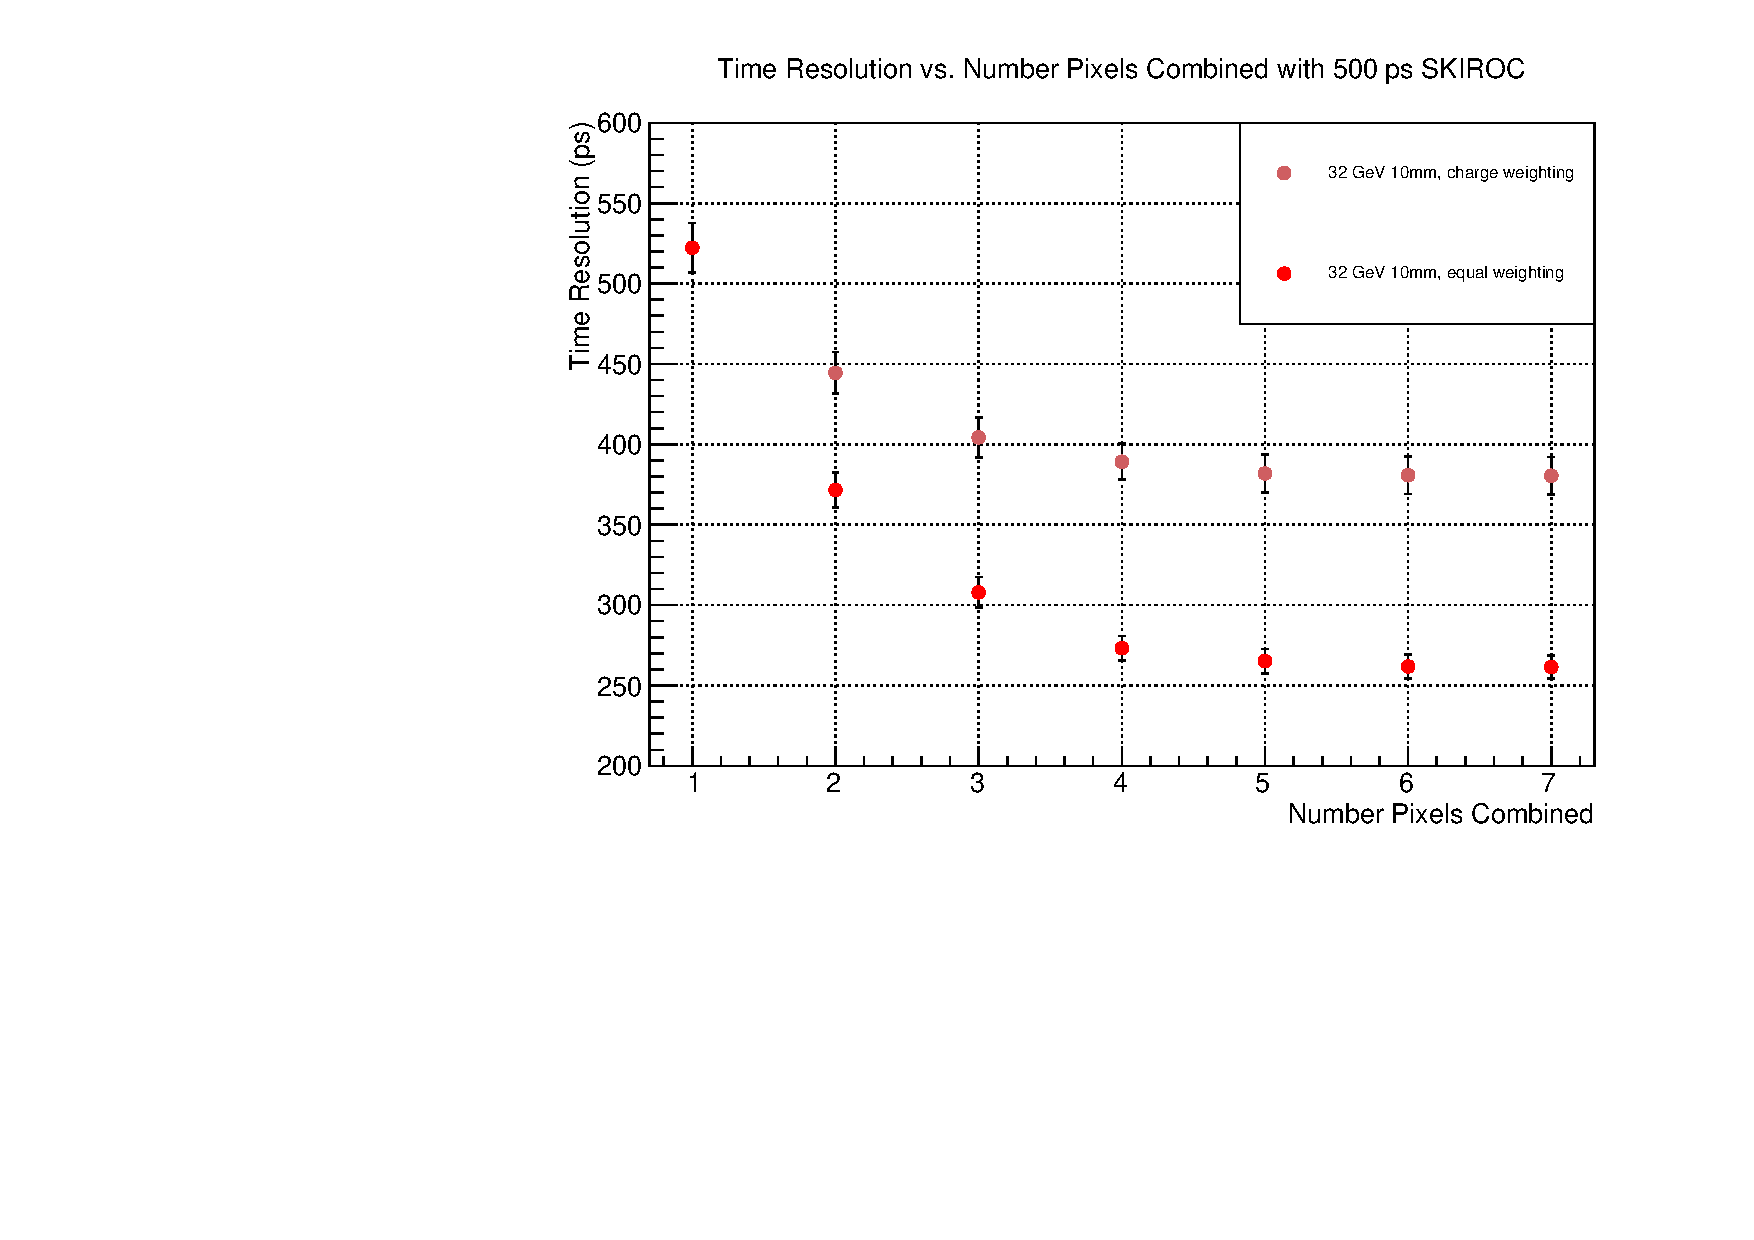
\includegraphics[width = 0.8\textwidth]{smearing_500_10mm}
\caption{Results of the SKIROC smearing analysis with 500 ps smearing. This is for the 10mm separation data, and is representative of the other distances with the 32 GeV electron beam.}
\label{500 smearing}
\end{figure*}

When a SKIROC modeling is done to represent the noise in the digitization of the signal, the time resolution is significantly improved when all 7 pixels are combined. The pixel combination gives an improvement of about 10ps (for 50ps smearing) and 250ps (for 500ps smearing) over the time resolution from the center pixel alone. For 50ps smearing, both equal pixel weighting and charge weighting result in approximately the same improvement, with charge weighting being slightly better. With 500ps smearing, equal pixel weighting improves the time resolution significantly more than charge weighting does.

These results demonstrate that with SKIROC noise, adding more pixels improves the time resolution. These additional pixels contain more information as compared to the central pixel alone, and therefore can improve the time resolution. In the case without smearing, the central pixel dominated the time resolution, and thus adding additional pixels did not improve the time resolution. 

The SKIROC modeling was done with a smearing of 500ps to examine the effects of pixel addition when all added pixels have a similar time resolution. When 500ps smearing is applied, the time resolution of each pixel is approximately the same - around 500ps. From Figure \ref{500 smearing} it is clear that when the time resolution is approximately equal in the pixels being combined, adding more pixels improves the time resolution quite significantly. Figure \ref{500 smearing} shows the time resolution after pixels are sorted according to the magnitude of charge contained (on an event-by-event basis), and then combined in this ordering. This is done with both an equal and charge pixel weighting. Equal weighting gives a lower time resolution than charge weighting for 500ps smearing, likely because when each pixel has a similar time resolution, no one pixel dominates the overall time resolution (as the central pixel previously did). With 50ps smearing, the time resolution decreases from about 55ps (with a single pixel) to 45ps (with all pixels combined); and 500ps smearing, the time resolution decreases from about 500ps to 250ps [Figures \ref{50 smearing} and \ref{500 smearing}]. These results are seen for all four absorber separation distances.

Similarly, a SKIROC modeling with 50ps and 500ps time smearing was done for the case where only the first ring of pixels are combined (the central pixel was not used). The first ring of pixels are pixels labeled 2 through 7 in Figure \ref{pico-sil}. In this case, the cuts applied to select events were on the Photek detector and on the charge and amplitude of the largest pixel in the first ring. If a pixel did not pass the charge and amplitude cuts ($>$ 0.01 V in amplitude, and $>$ 1 pC of charge), it was added with a weight of 0. Pixels were combined in order of charge contained, and were all weighted equally in the time resolution determination. The results are shown in Figure \ref{500 and 50 smearing no center}, and it is seen that adding pixels improves the time resolution. Most of the improvement is seen in combining the first two pixels, likely because most of the charge is contained in these pixels. 

%Similarly, a SKIROC modeling with 50ps and 500ps time smearing was done for the case where only the first ring of pixels are combined (the central pixel was not used). The first ring of pixels are pixels labeled 2 through 7 in Figure \ref{pico-sil}. In this case, the cuts applied to select events were on the Photek detector and on the charge and amplitude of the largest pixel in the first ring. If a pixel did not pass the charge and amplitude cuts ($>$ 0.01 V in amplitude, and $>$ 1 pC of charge), it was added with a weight of 0. Pixels were combined in order of charge contained, and were all weighted equally in the time resolution determination. The results are shown in Figure \ref{500 and 50 smearing no center}, and it is seen that adding pixels improves the time resolution. Most of the improvement is seen in combining the first two pixels, likely because most of the charge is contained in these pixels. 

\begin{figure*}[!htbp]
\centering
\subfigure[Time resolutions for combinations of pixels in the first ring with 50ps SKIROC smearing applied.]{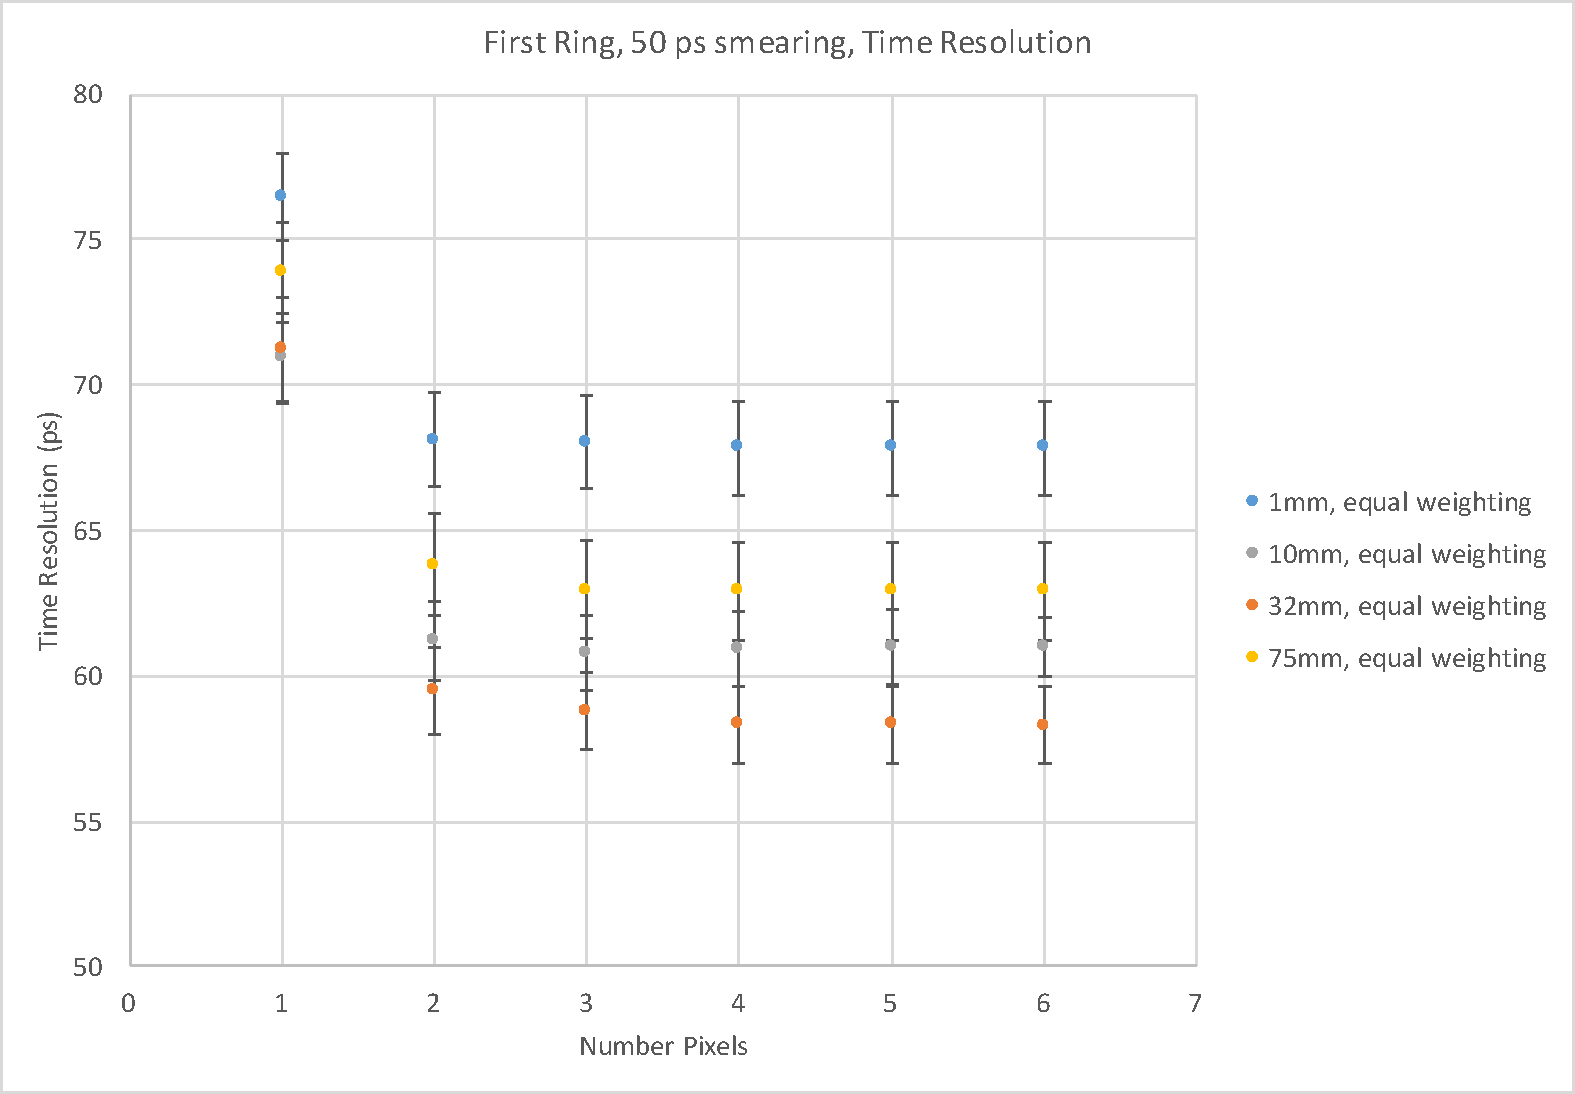
\includegraphics[width = 0.47\textwidth]{50ps_distances_ring}} 
\subfigure[Time resolution for combinations of pixels in the first ring with 500ps SKIROC smearing applied. The 1mm and 75mm points are in very similar positions, and the 10mm and 32mm points are also in very similar positions.]{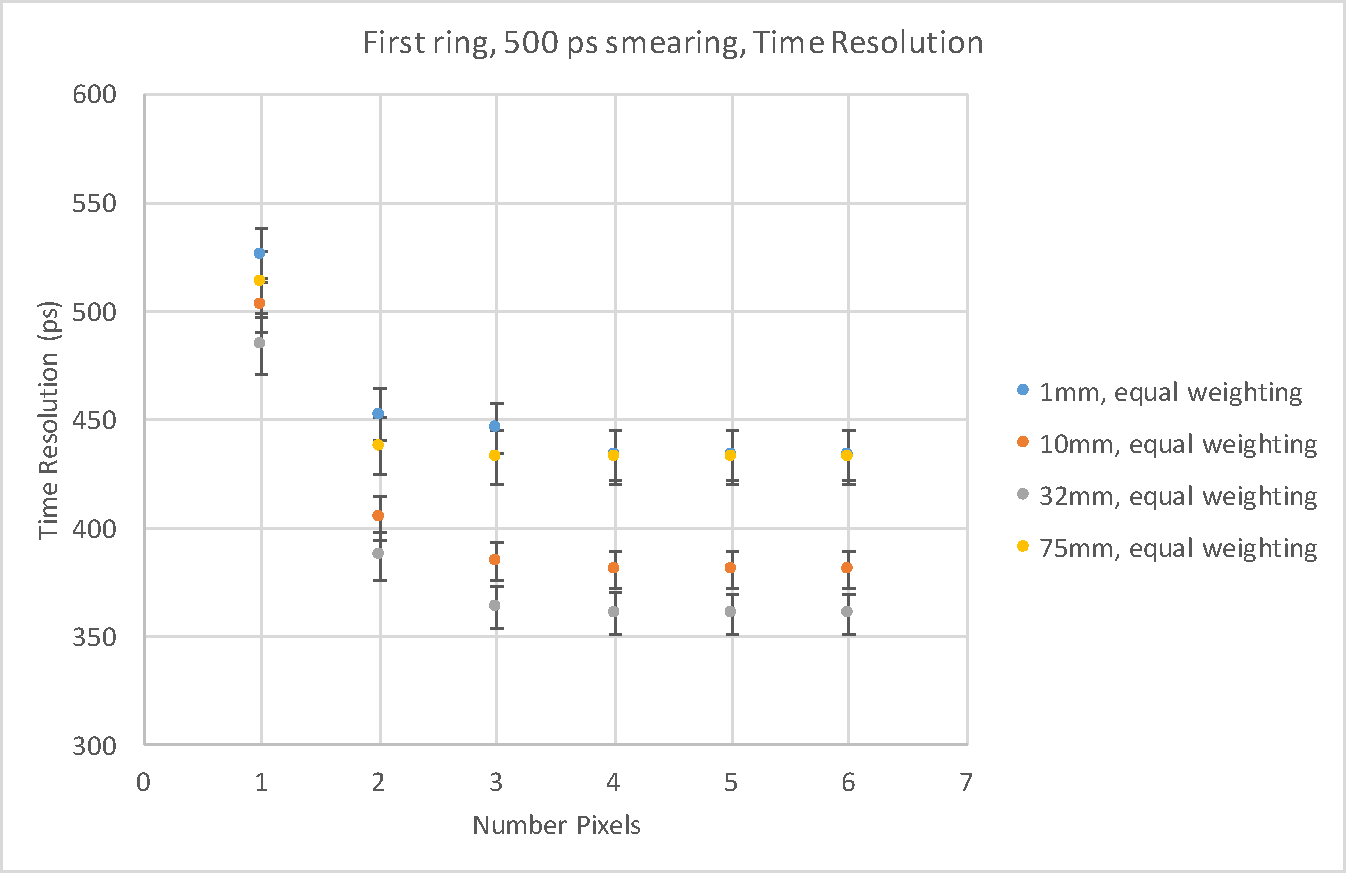
\includegraphics[width = 0.5\textwidth]{500ps_distances_ring}} 
\caption{The time resolution (in ps) plotted vs. the number of pixels combined with both the 50 and 500ps SKIROC smearing modeling. In both cases, pixels are combined in order of how much energy they contain. In both cases, time resolution is significantly improved by the combination of all 7 pixels. This is for the first ring of pixels - the central pixel was not used for this time resolution determination. \textit{Preliminary results.}}
\label{500 and 50 smearing no center}
\end{figure*}

\subsection{Time Resolution Improvement and Pixels Combined}

It is expected that the time resolution is related to the number of pixels combined by

\begin{equation}
\frac{\text{initial time resolution}}{\text{final time resolution}} = \sqrt{N}
\label{square root N}
\end{equation}

where $N$ is the number of pixels combined. (Note: this holds if all pixels have a similar signal to noise ratio - which is true when the 500ps SKIROC smearing is applied. In this case, the signal to noise has been artificially made the same between channels by applying this smearing.)

As noted before, for this pixel combination method when all pixels are combined, often less than 7 pixels are combined, based on which pixels pass the cuts (pixels that do not pass the cuts are added with a weight of 0 so the event can still be used). This is why $N$, the number of pixels combined, in Table \ref{table:N values} is not 7, the total number of pixels combined. However, the average number of pixels combined per event is a good representation of $N$, and is determined by the mean of the histograms shown in [Figure \ref{pixels average}].

When Equation \ref{square root N} is used with the 50ps smearing analysis for 32 GeV and 32 mm separation, the calculated $N$ value is 1.6, while the value from the mean of the histogram is 4. This difference indicates that the central pixel is still dominant in the case of 50 ps smearing. However, 500 ps smearing means that all pixels have approximately the same time resolution, and thus the pixel combination should follow Equation \ref{square root N}.

When the time resolutions from the various separation distances are used (with the 500ps smearing with equal weighting), the time resolutions and calculated values of $N$ are listed in Table \ref{table:N values}. The average number of pixels combined per event is a good representation of $N$, and is determined by the mean of the histograms shown in [Figure \ref{pixels average}]. These average $N$ values are listed in Table \ref{table:cuts}.

\begin{centering}
\begin{table*}[!htbp]
  \begin{tabular}{ | c | c | c | c | c | c | }
    \hline
    \multirow{2}{*} {Beam Energy (GeV)} & Separation & Initial time & Final time & N & N \\
  & Distance (mm) & resolution (ps) & resolution (ps) & (calculated) & (histogram) \\ \hline
    32 & 1 & 515.9 & 315.2 & 2.7 & 2.6 \\ \hline
    32 & 10 & 522.3 & 261.5 & 4.0 & 3.8 \\ \hline
    32 & 32 & 489.5 & 242.3 & 4.1 & 4.0 \\	\hline
    32 & 75 & 489.0 & 302.4 & 2.6 & 2.9 \\ \hline
    16 & 1 & 497.2 & 341.6 & 2.1 & 2.3 \\ \hline
    8 & 1 & 502.8 & 415.6 & 1.5 & 1.7 \\ \hline
  \end{tabular}
\caption[Table caption text]{Table of calculated $N$ value from the initial and final time resolution, and the $N$ value determined from the average of the number of pixels combined histogram (Figure \ref{pixels average}).}
\label{table:N values}
\end{table*}
\end{centering}

\begin{figure*}[!htbp]
\centering
\subfigure[Histogram of largest number of pixels passing the charge and amplitude cuts when the absorber is at 1mm, 32 GeV.]{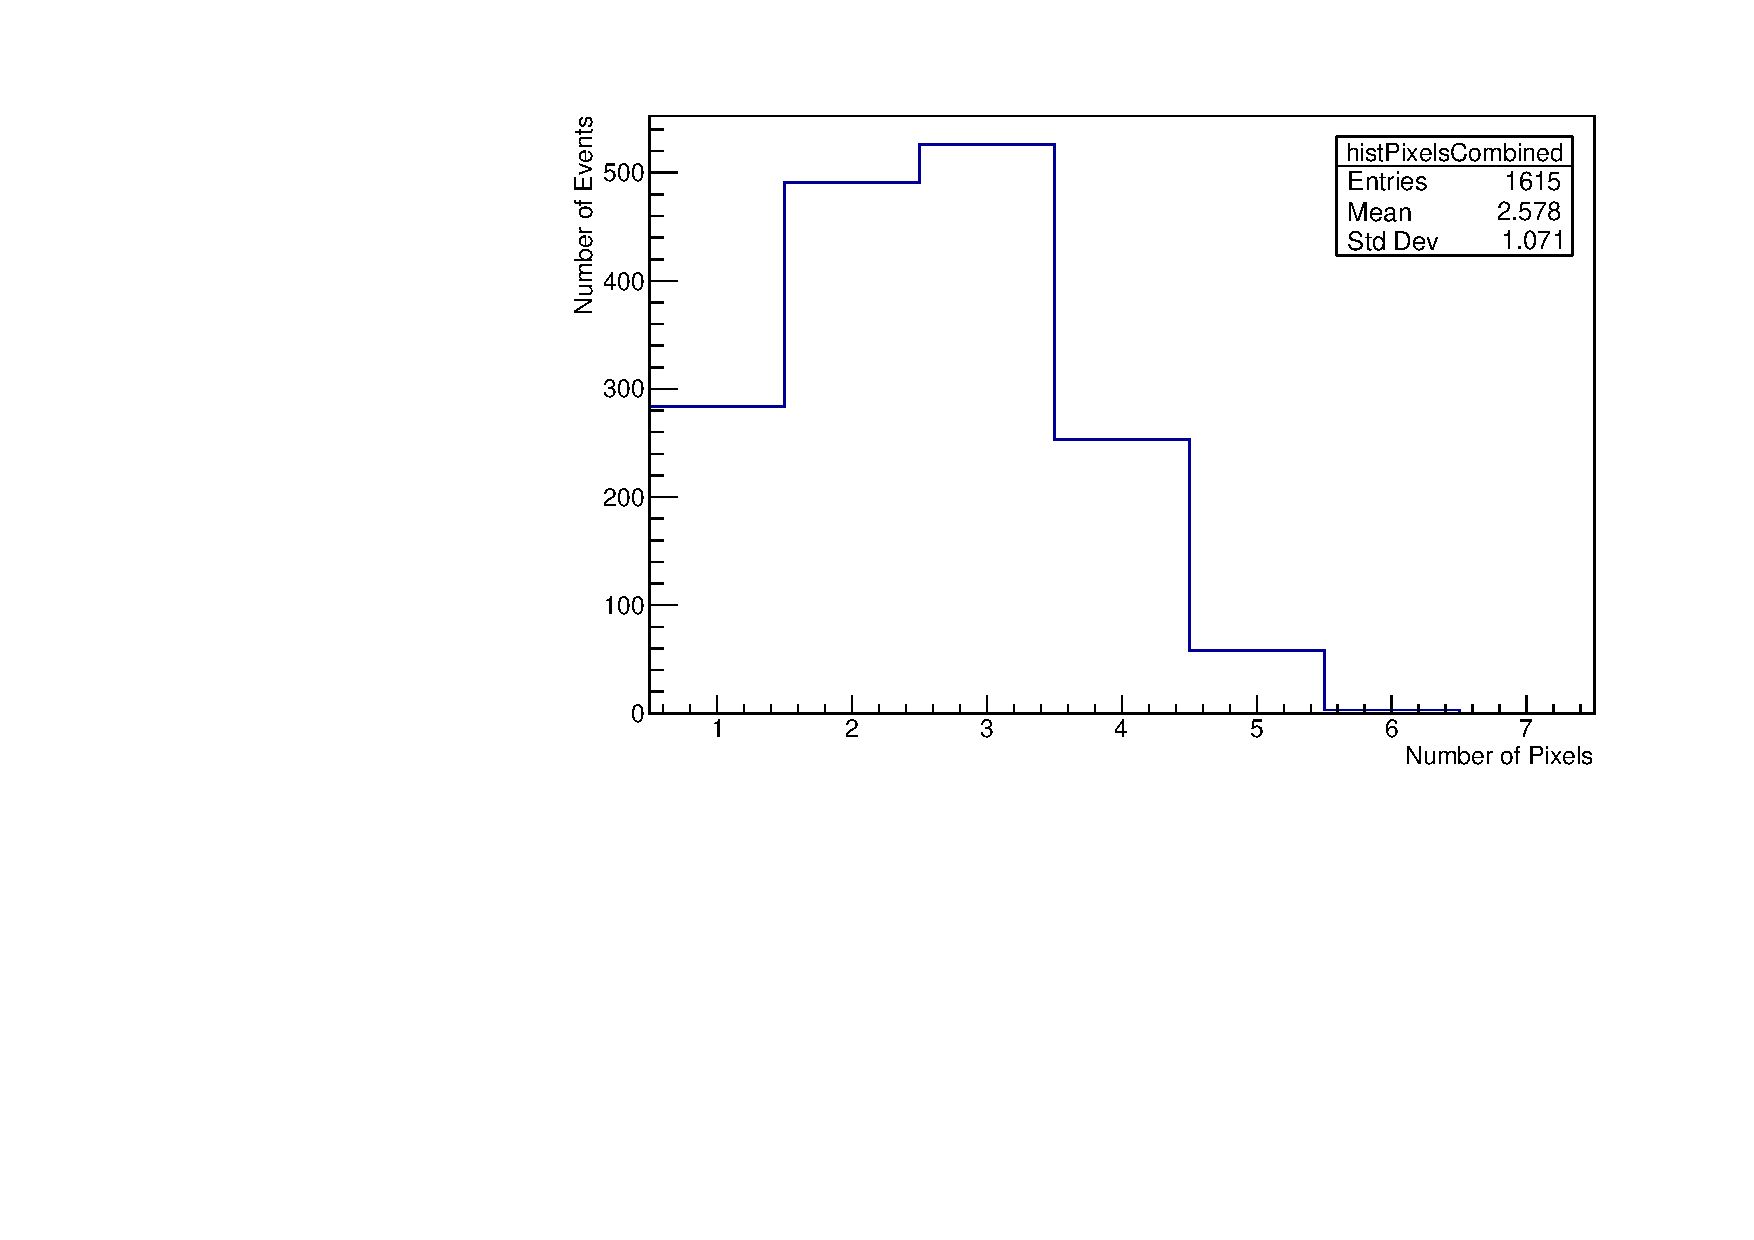
\includegraphics[width = 0.45\textwidth]{combined1}} 
\subfigure[Histogram of largest number of pixels passing the charge and amplitude cuts when the absorber is at 10mm, 32 GeV.]{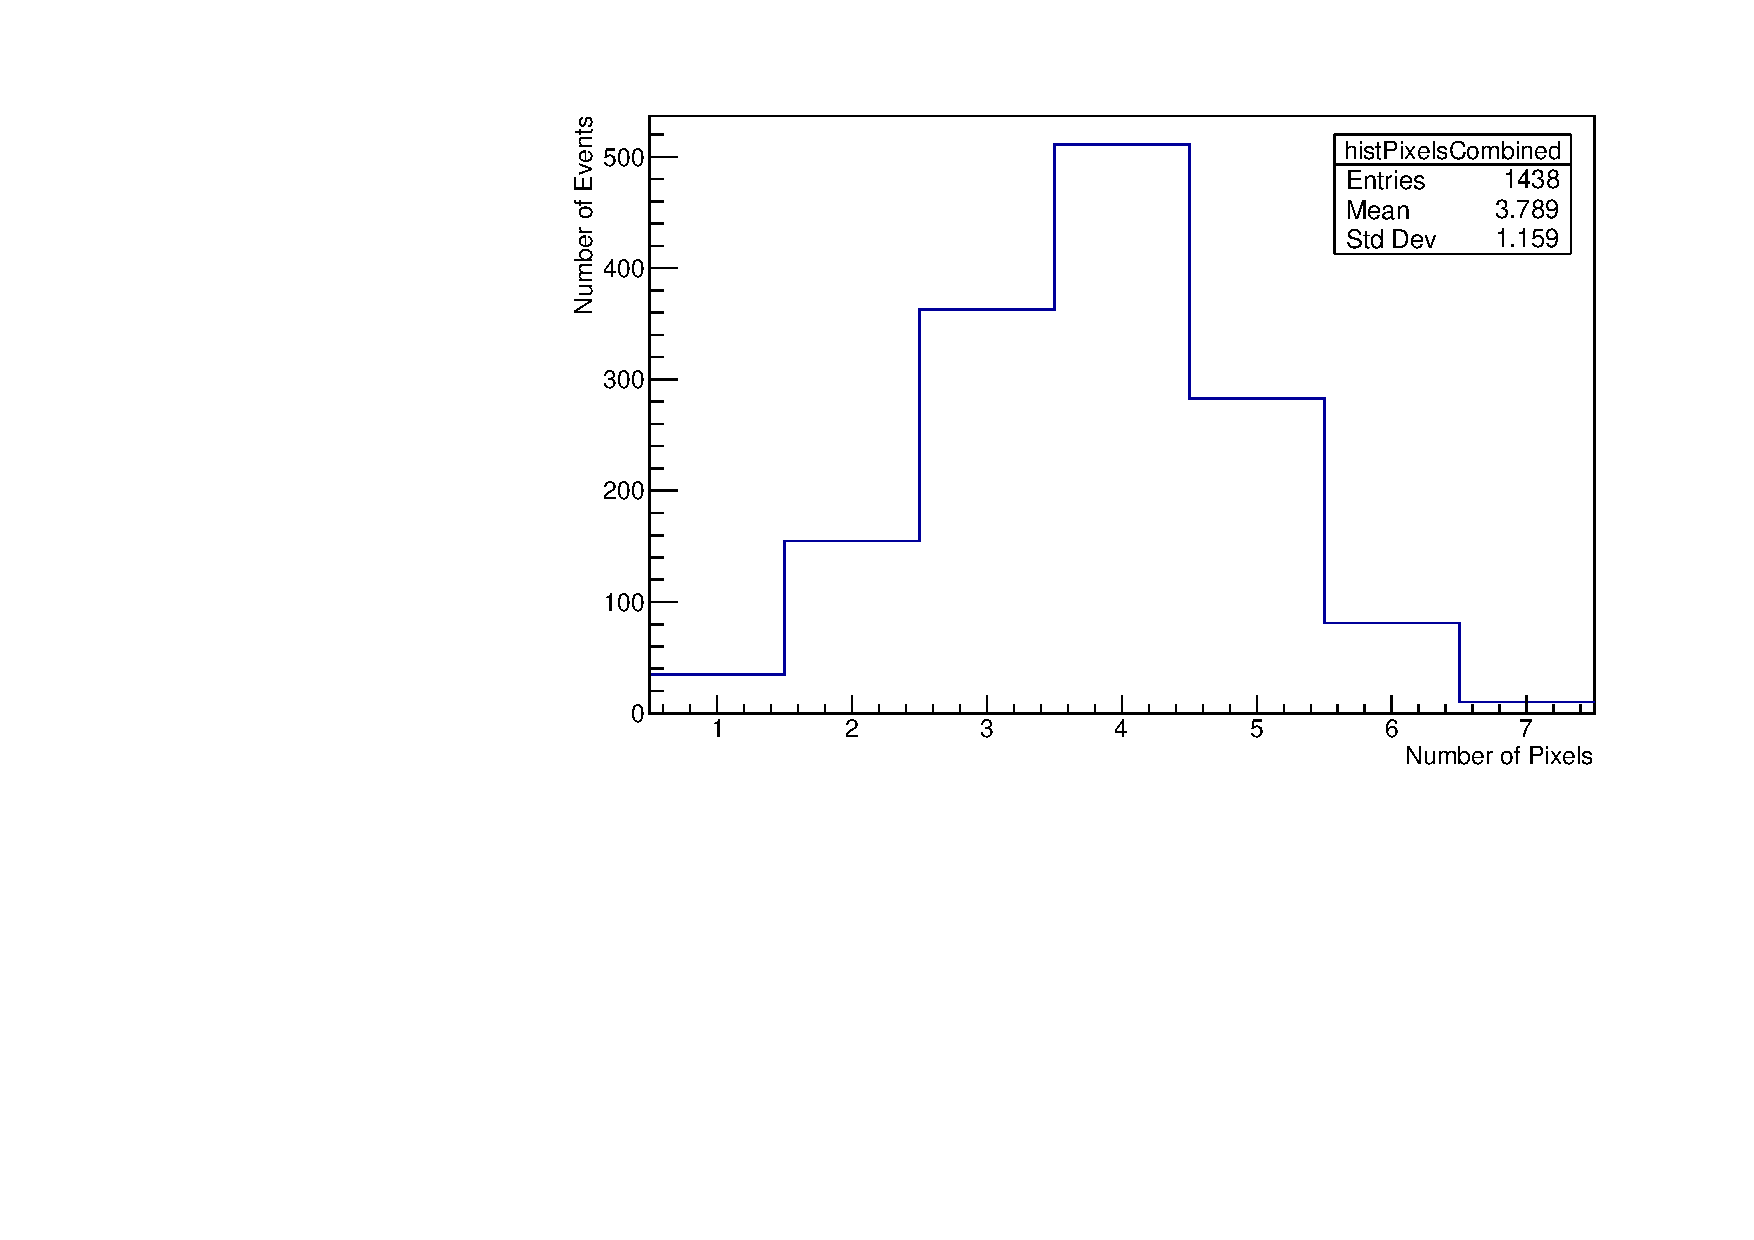
\includegraphics[width = 0.45\textwidth]{combined10}} 
\subfigure[Histogram of largest number of pixels passing the charge and amplitude cuts when the absorber is at 32mm, 32 GeV.]{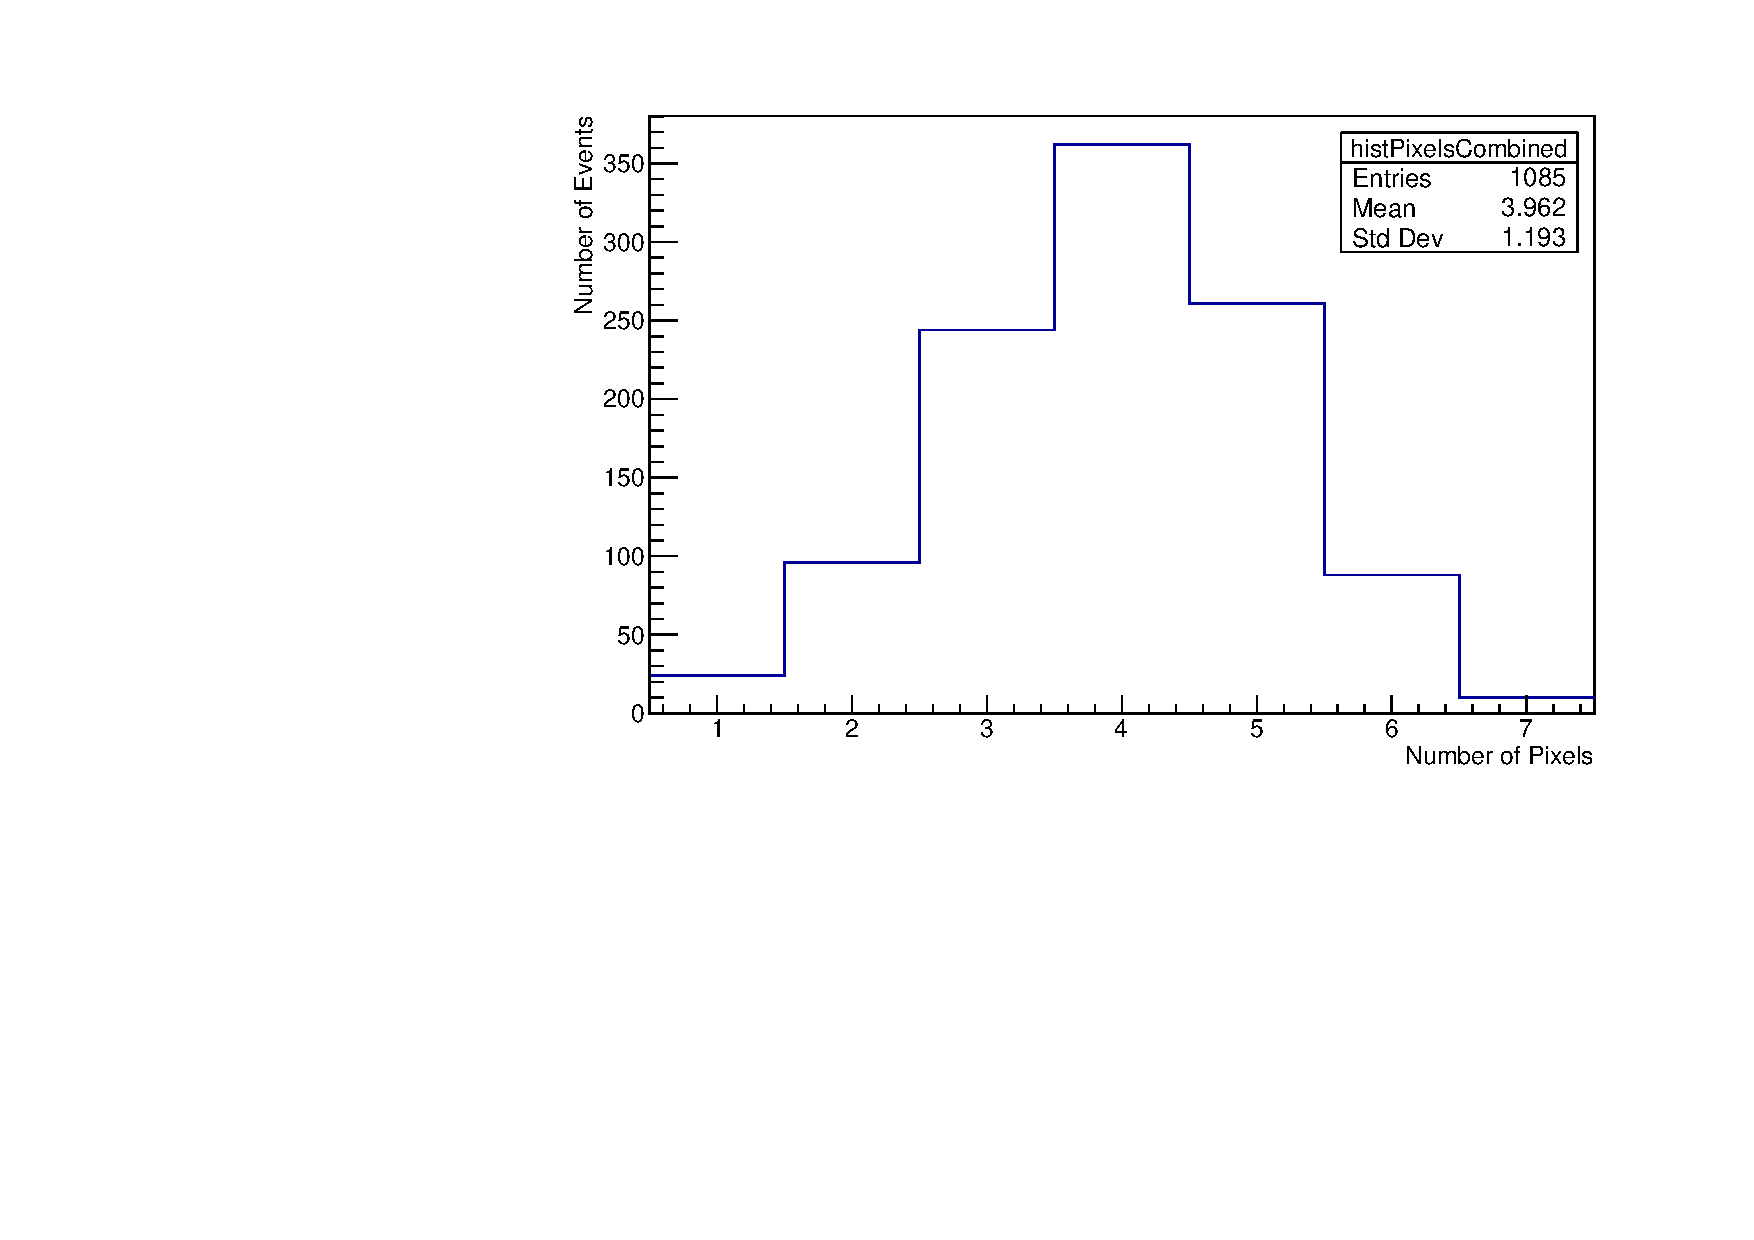
\includegraphics[width = 0.45\textwidth]{combined32}} 
\subfigure[Histogram of largest number of pixels passing the charge and amplitude cuts when the absorber is at 75mm, 32 GeV.]{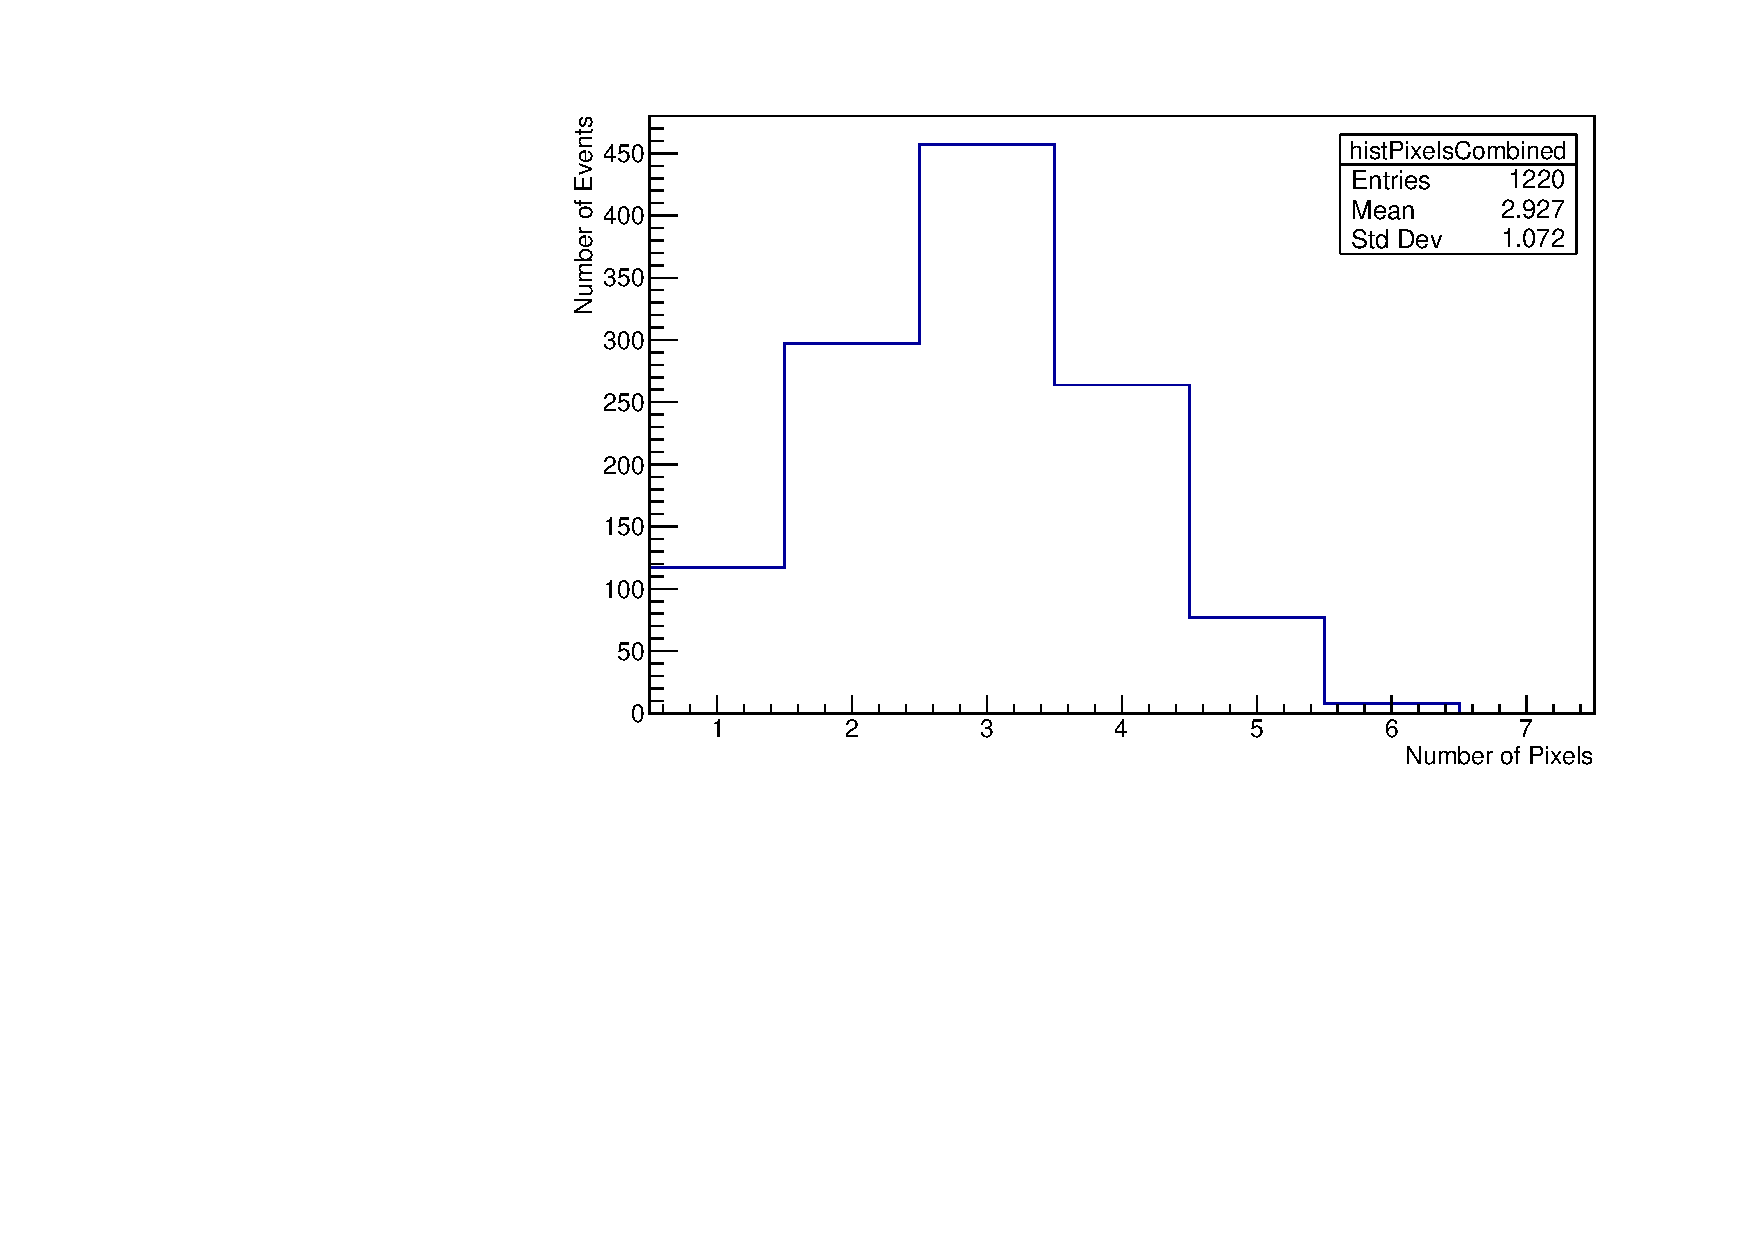
\includegraphics[width = 0.45\textwidth]{combined75}} 
\subfigure[Histogram of largest number of pixels passing the charge and amplitude cuts when the absorber is at 1mm, 16 GeV.]{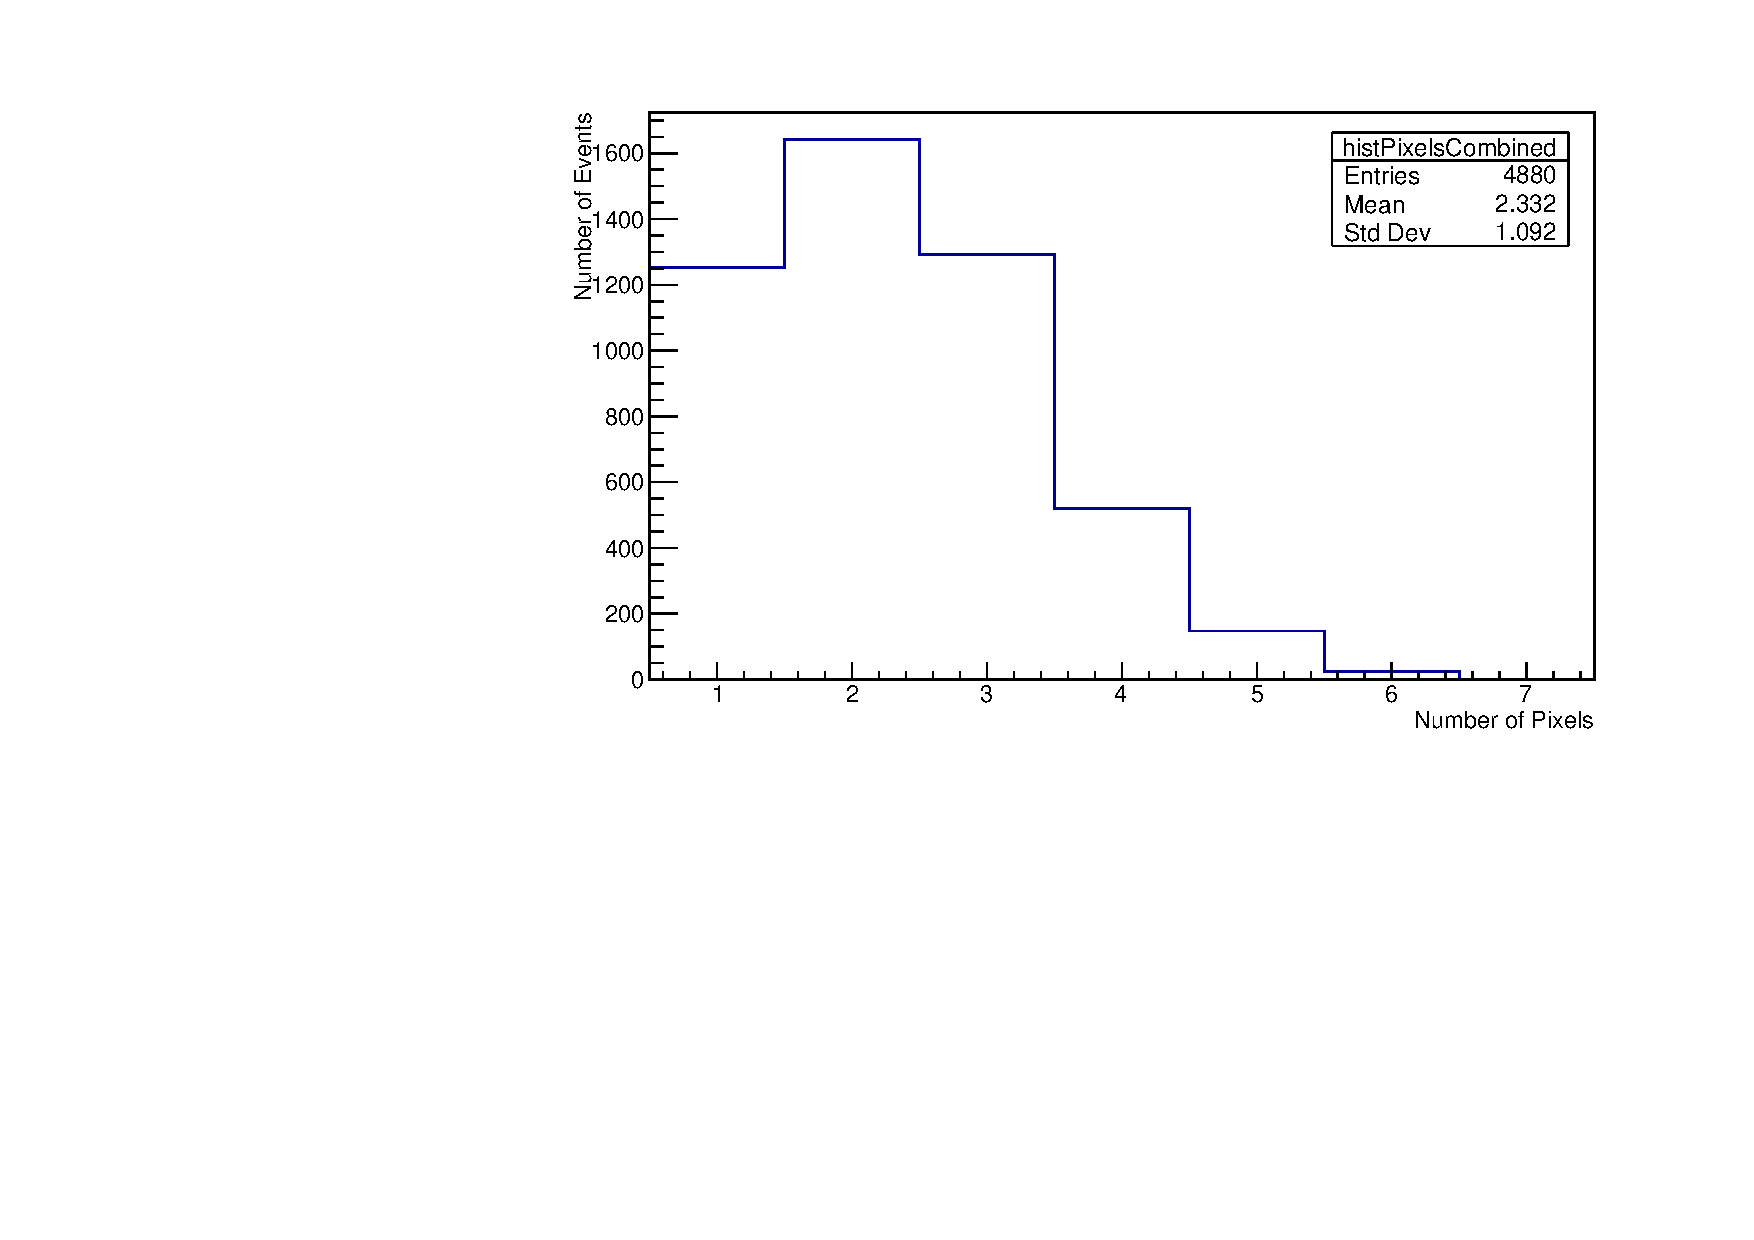
\includegraphics[width = 0.45\textwidth]{16_1mm_pixels}}
\subfigure[Histogram of largest number of pixels passing the charge and amplitude cuts when the absorber is at 1mm, 8 GeV.]{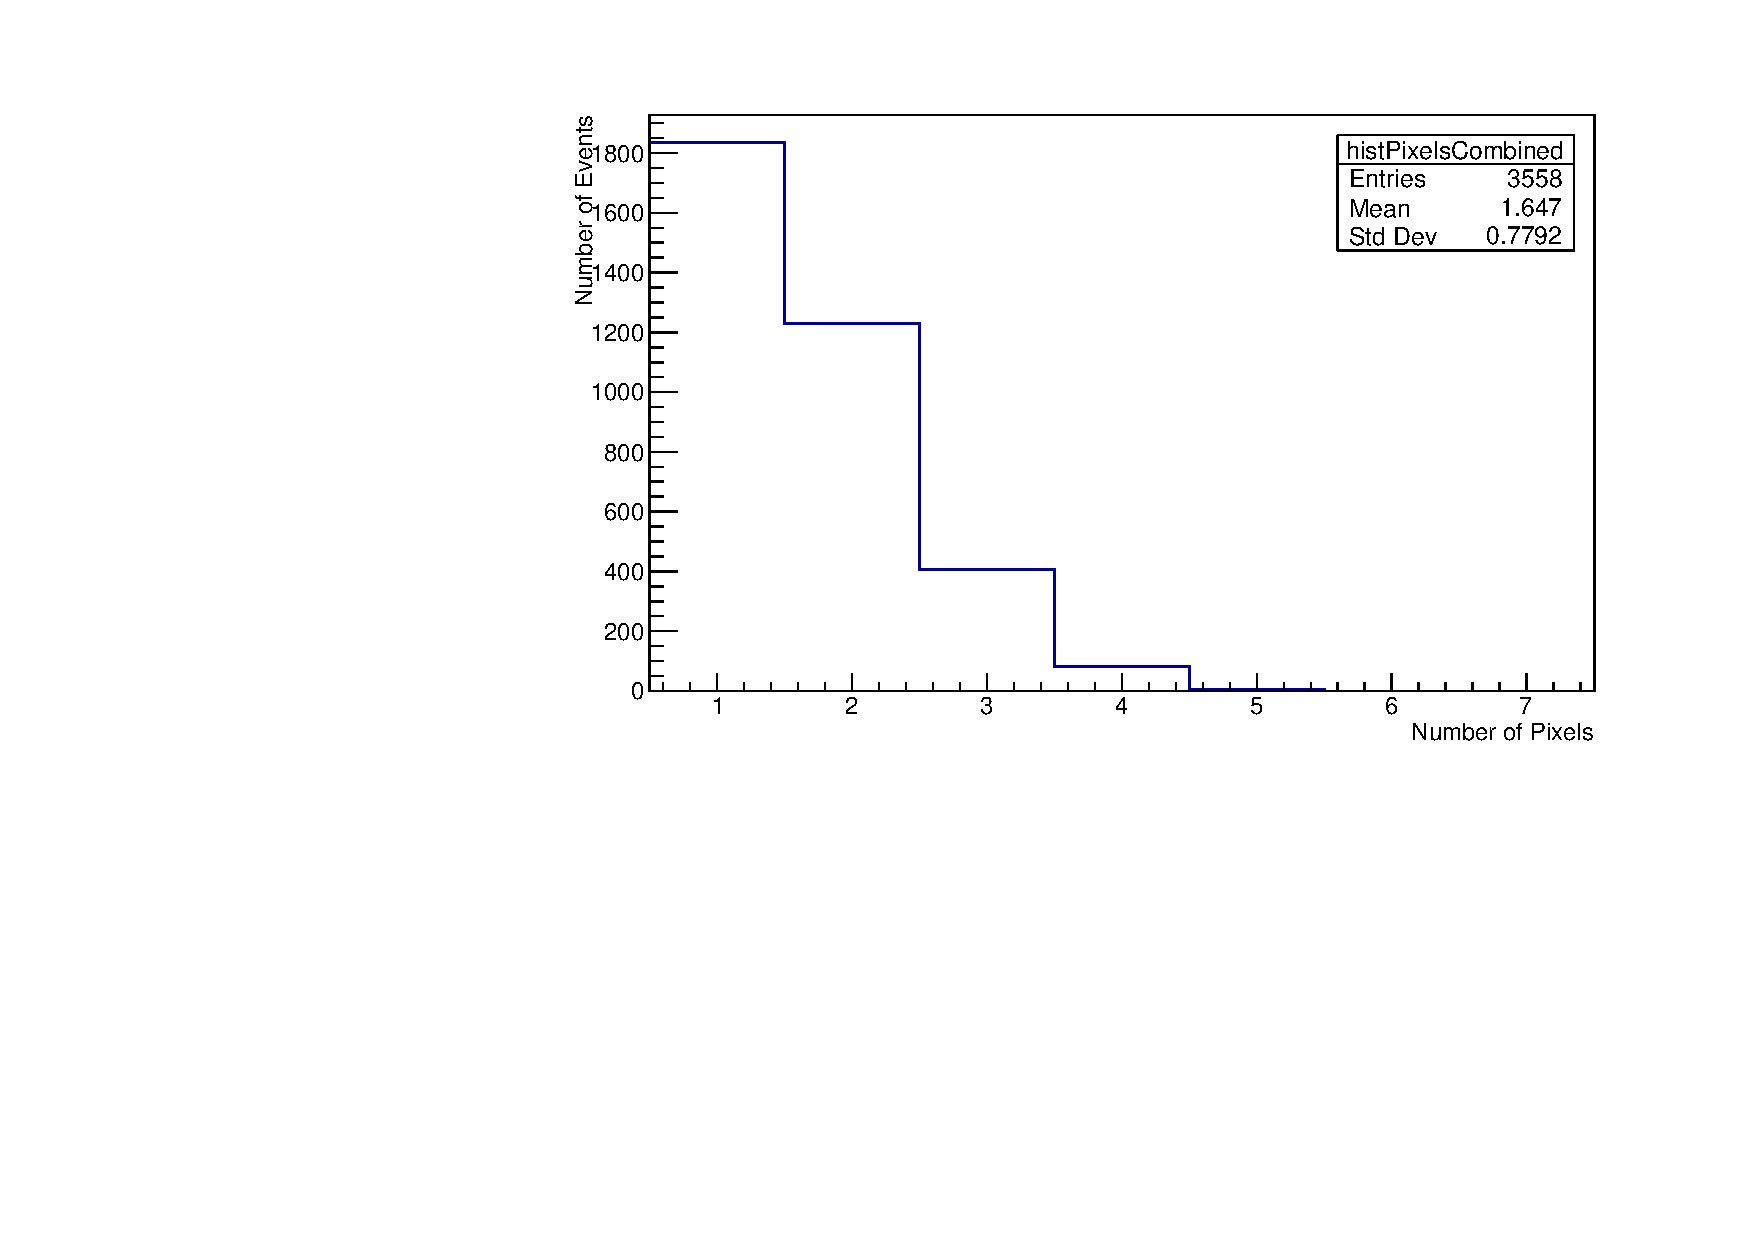
\includegraphics[width = 0.45\textwidth]{8_1mm_pixels}} 
\caption{The number of pixels passing the charge and amplitude cuts for each absorber distance. Generally, around 3 pixels pass the cuts for a given event. The mean of these histograms is taken as a good representation of the number of pixels combined for each analysis.}
\label{pixels average}
\end{figure*}

\begin{figure}[!htbp]
\centering
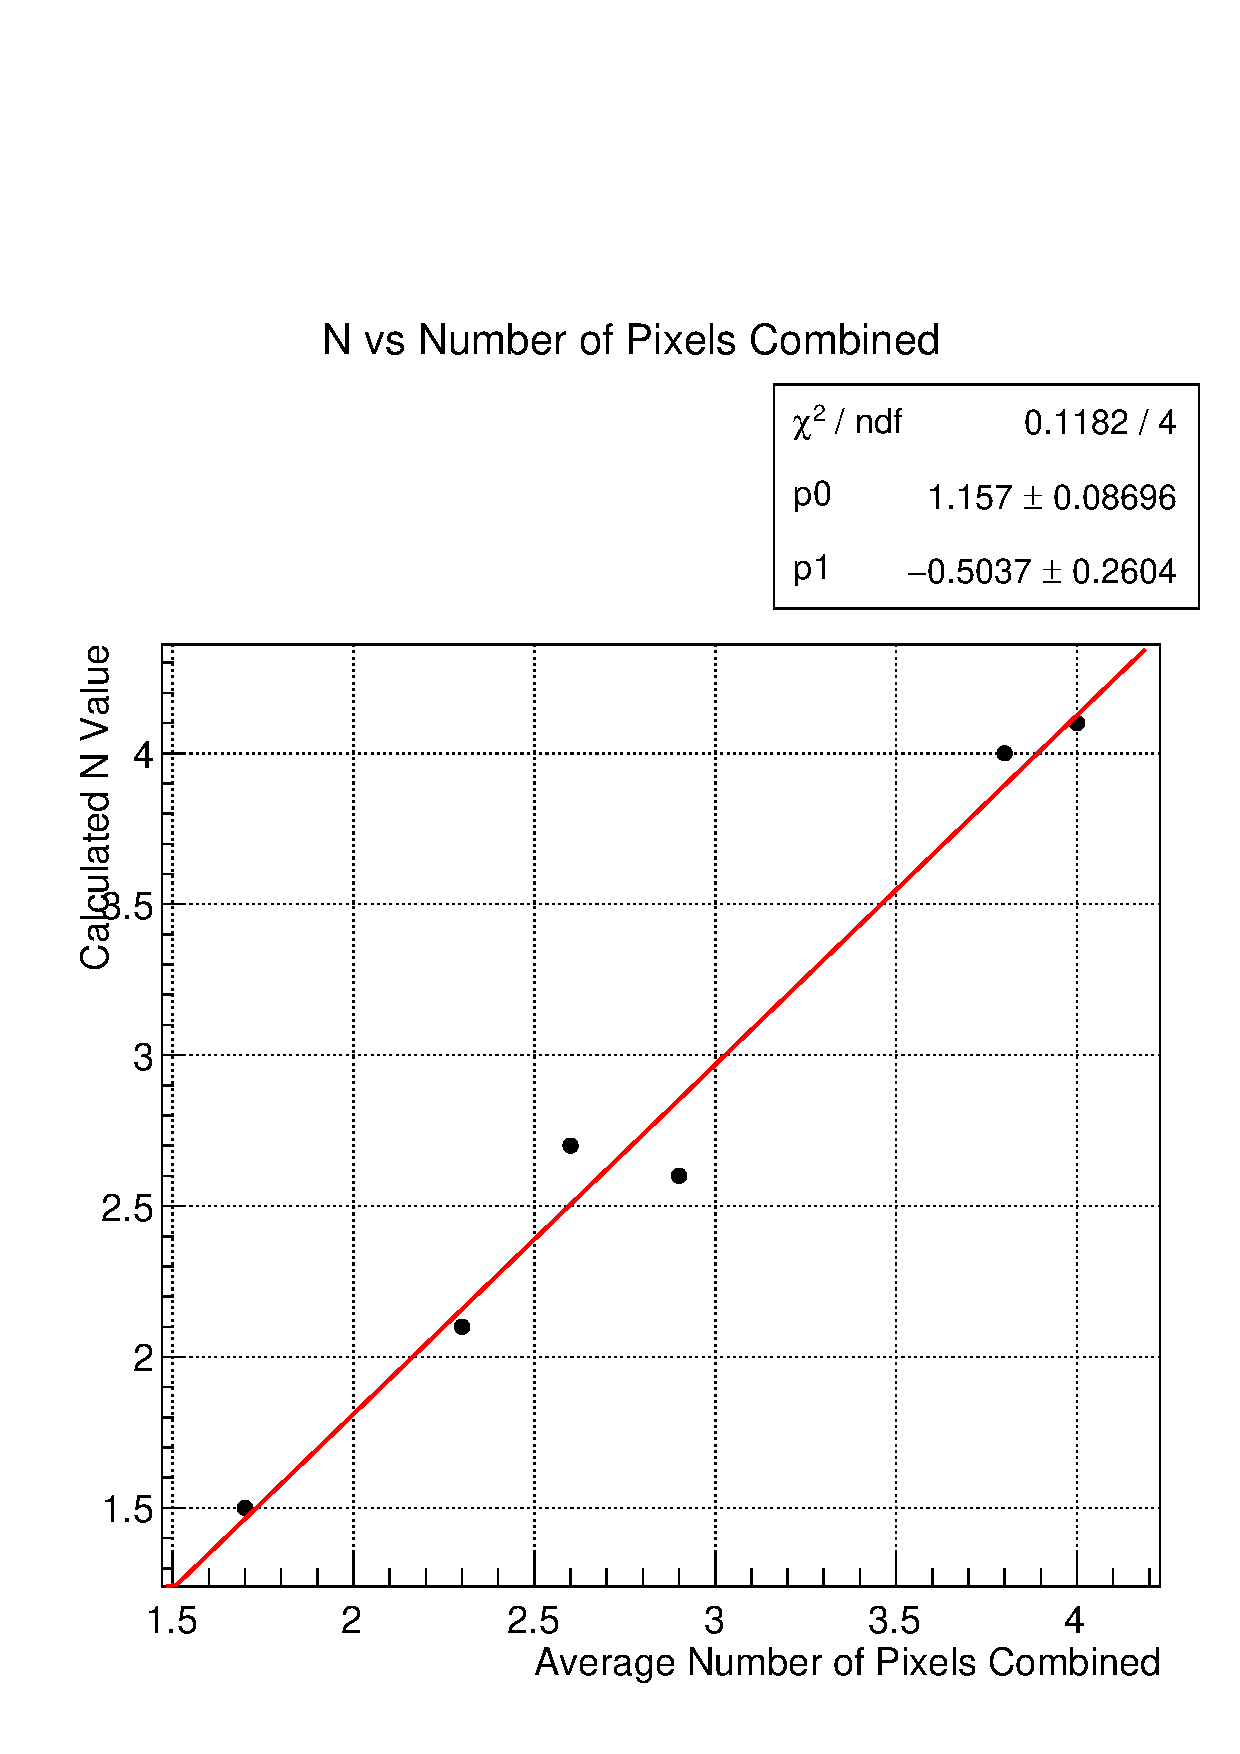
\includegraphics[width = 0.45\textwidth]{time_res_n}
\caption{Plot of the calculated $N$ value (from the initial and final time resolutions) and the $N$ valued determined from the average of the histograms in Figure \ref{pixels average}.}
\label{linear fit N}
\end{figure}

This result shows that, as predicted by Equation \ref{square root N}, the time resolution improves as $\sqrt{N}$, where $N$ is interpreted as the average number of pixels with signal, given that the time resolution of each pixel individually is similar. When a linear fit is done, the chi squared value is very low, and the fit is 

\begin{equation}
1.157 \cdot N_{average} - 0.5037 = N_{calculated}
\end{equation}

Thus, the SKIROC analysis has shown that when pixels have similar time resolution, combining pixels improves the time resolution by $\sqrt{N}$. With more active pixels, this improvement might be seen with no smearing, since a single pixel would not dominate the time resolution.

\subsection{Time Resolution and Beam Energy}

Understanding the relationship between beam energy and time resolution is important as in the CMS detector, particles with varying energies will be observed. Thus, an understanding of the time resolution dependence on event energy is needed to further characterize the time resolution capabilities of the HGC detector.

It is expected that for a calorimeter, the time resolution has an inverse square dependence on the beam energy, as shown by Equation \ref{equation:energy}

\begin{equation}
\frac{p_0}{\sqrt{Energy}} + p_1 = \text{time resolution}
\label{equation:energy}
\end{equation}

The time resolution dependence on beam energy is evaluated. The time resolution determined from the combination of all 7 pixels for various beam energies (at a separation distance of 1mm) vs the beam energy is plotted in Figure \ref{energy fits}. The time resolution is expected to fit to $\frac{p_0}{\sqrt{E}} + p_1$ [Equation \ref{equation:energy}]. This fit is done for the data from 32, 16, and 8 GeV, with all pixels combined in Figure \ref{energy fits}.

\begin{figure*}[!htbp]
\centering
\subfigure[Time resolution with no smearing, charge weighting, all pixels combined for the three beam energies.]{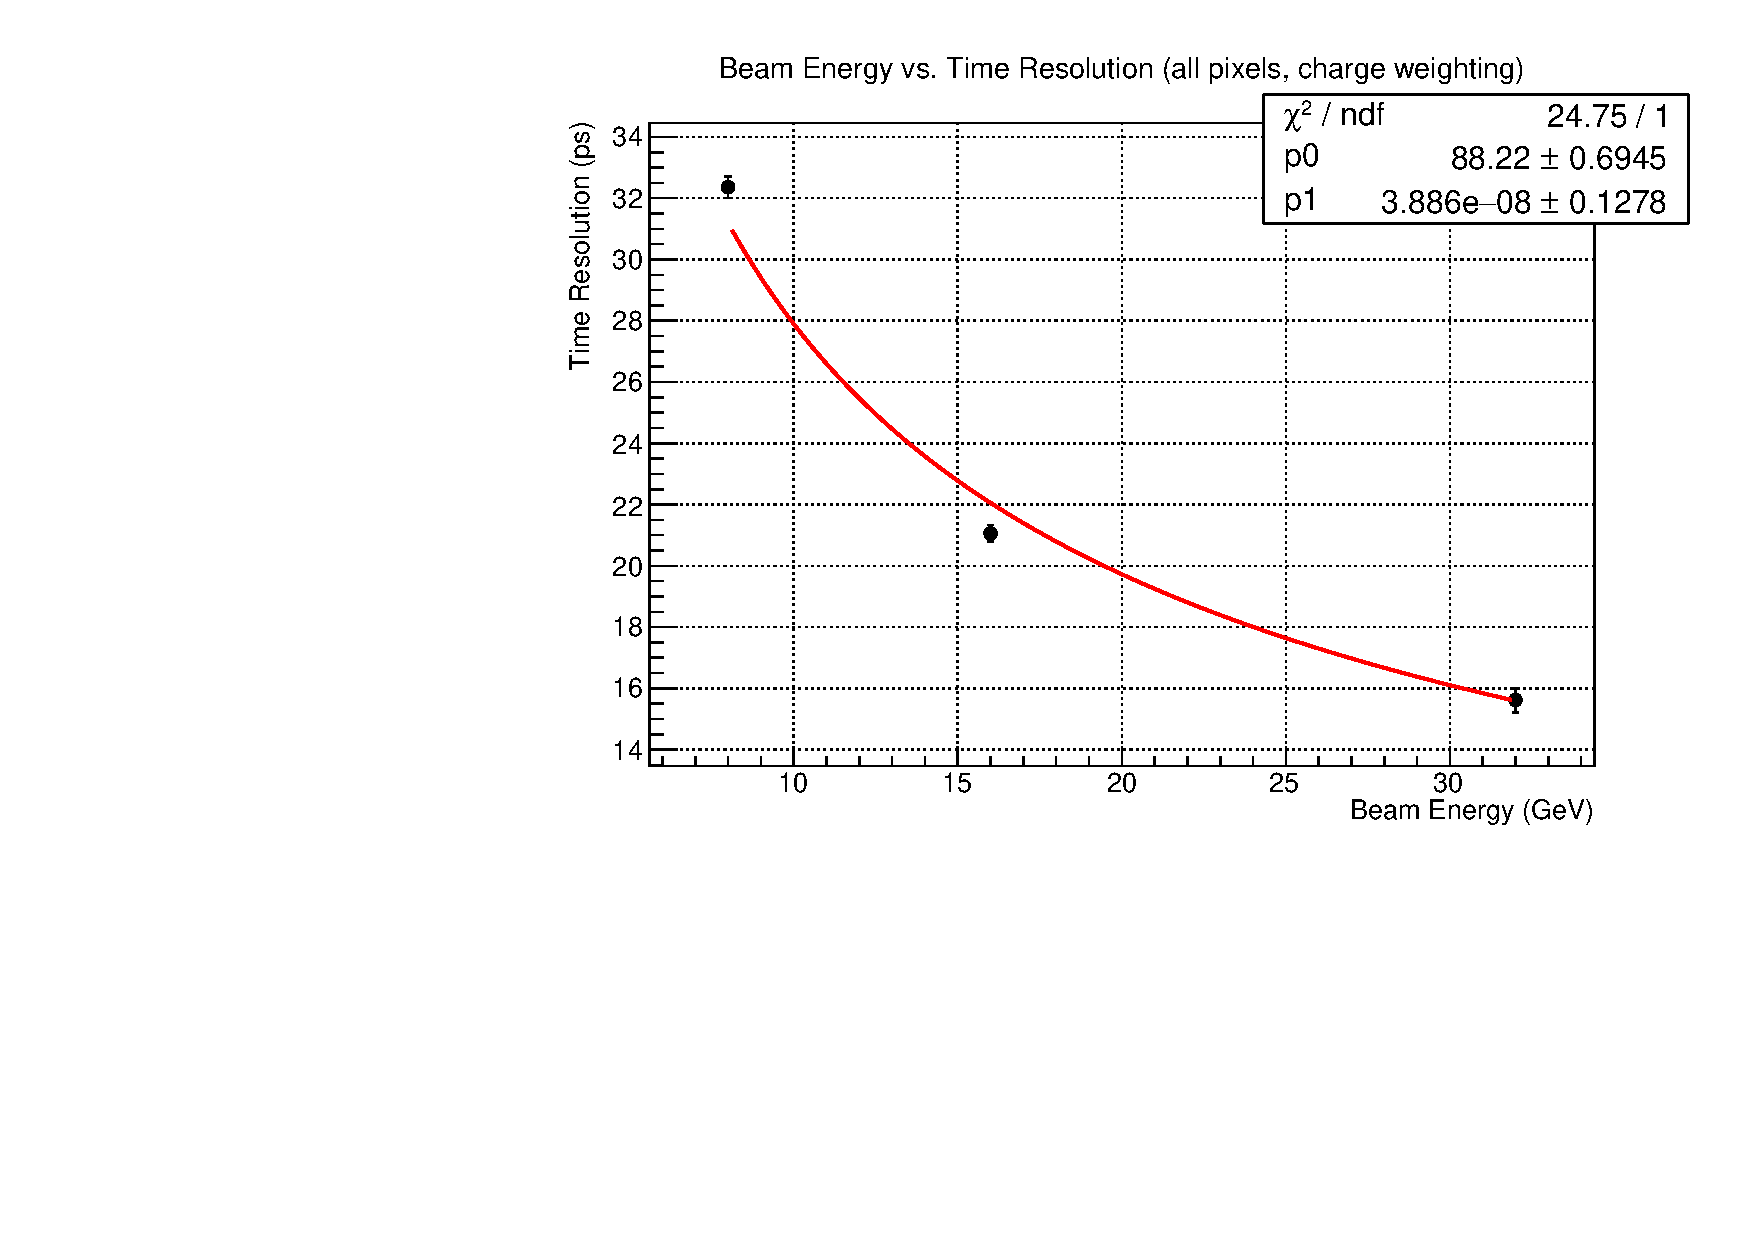
\includegraphics[width = 0.3\textwidth]{no_smearing}}
\hspace{3mm}
\subfigure[Time resolution with 50 ps smearing, equal weighting, all pixels combined for the three beam energies.]{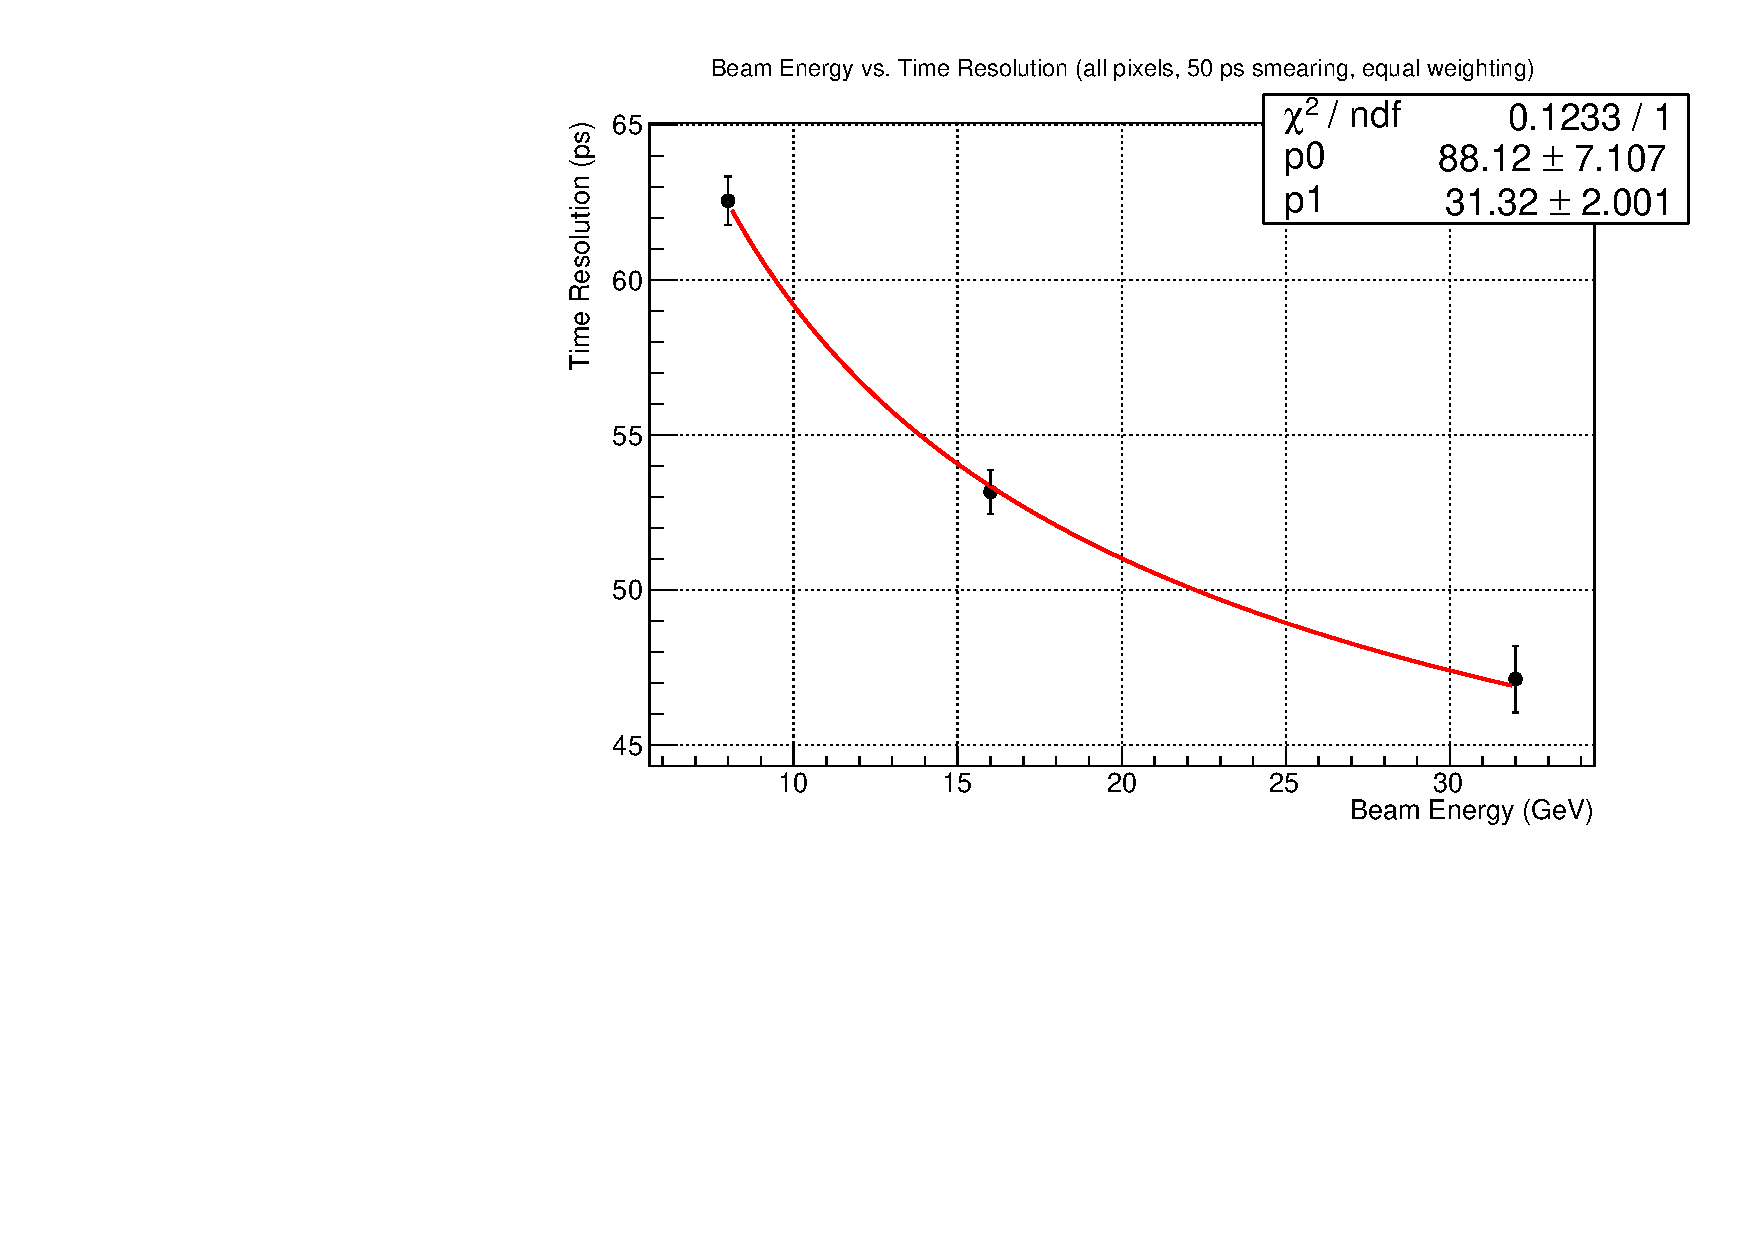
\includegraphics[width = 0.3\textwidth]{50_ps_smearing}}
\hspace{3mm}
\subfigure[Time resolution with 500 ps smearing, equal weighting, all pixels combined for the three beam energies.]{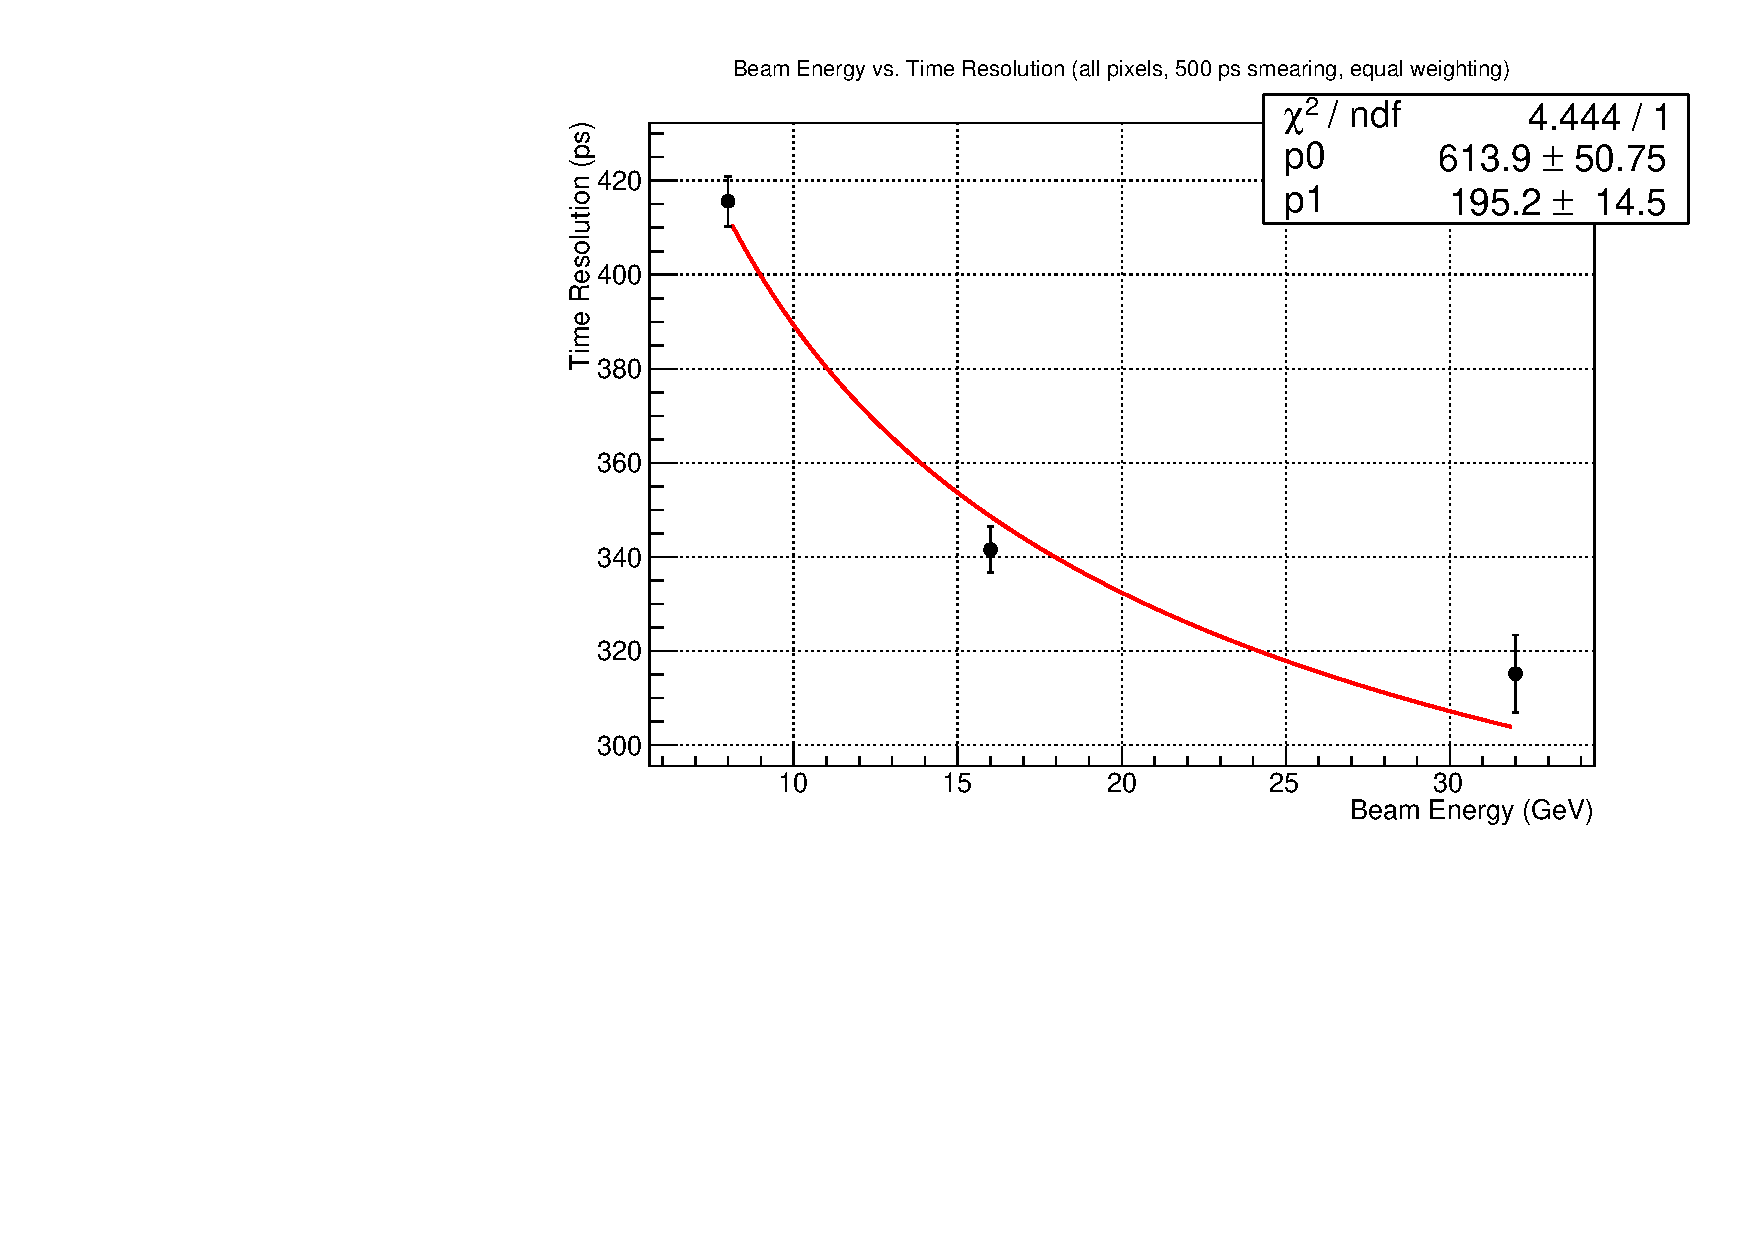
\includegraphics[width = 0.3\textwidth]{500_ps_smearing}}
\caption{Beam energy vs. time resolution with fits to $\frac{p_0}{\sqrt{E}} + p_1$. The time resolution fits the $\frac{p_0}{\sqrt{E}} + p_1$ model well.}
\label{energy fits}
\end{figure*}

With 50 and 500 ps smearing, the data fits Equation \ref{equation:energy} well [Figure \ref{energy fits}]. For 50 ps smearing, the constant term indicates that the theoretical time resolution achievable (as the beam energy is increased) is 31 ps. For 500 ps smearing, this value is 195 ps. However, the data does not fit to Equation \ref{equation:energy} without smearing [Figure \ref{energy fits}a] well, and the constant term is 0 (not physically possible). This indicates that more data is needed at higher beam energies and at beam energies between the current measurements at 8, 16, and 32 GeV to determine the trend in time resolution better.

Additionally, the constant term in the fits in Figure \ref{energy fits} indicate the theoretical limit to the time resolution, if the beam energy could be increased. However, this further shows that the no smearing data does not fit this time resolution - beam energy relationship well, as the constant term is 0. However, for the data with 50 ps SKIROC smearing applied, the constant term is 31 ps - indicating that with the HGC detector, the goal time resolution of 30 ps is achievable. In the case where multiple pixels have a similar time resolution or the shower covers a larger area, a lower time resolution could likely be achieved.

\subsection{Events Selected by Event Charge}

Figure \ref{2D histogram} plots the timestamp vs. the charge contained in an event in a 2D histogram. To investigate the time resolution dependence on event energy, events are selected in energy bins and the time resolution is determined from these events.

Since there is a slight time of flight dependence on charge, a cubic correction was applied to the 2D histogram before the charge event selection cuts were made. Additionally, in some cases, there were events that observed two electrons. Therefore, one of the electrons was observed with a very large timestamp value, and these events were removed manually in the dat2root conversion, since the current code is not designed to analyze this. Events with a $\Delta t > 0.01$ ps were removed (this was around 0.1\% of events). A corrected plot of the 2D timestamp to charge histogram is shown in Figure \ref{2D histogram}.

\begin{figure*}[!htbp]
\centering
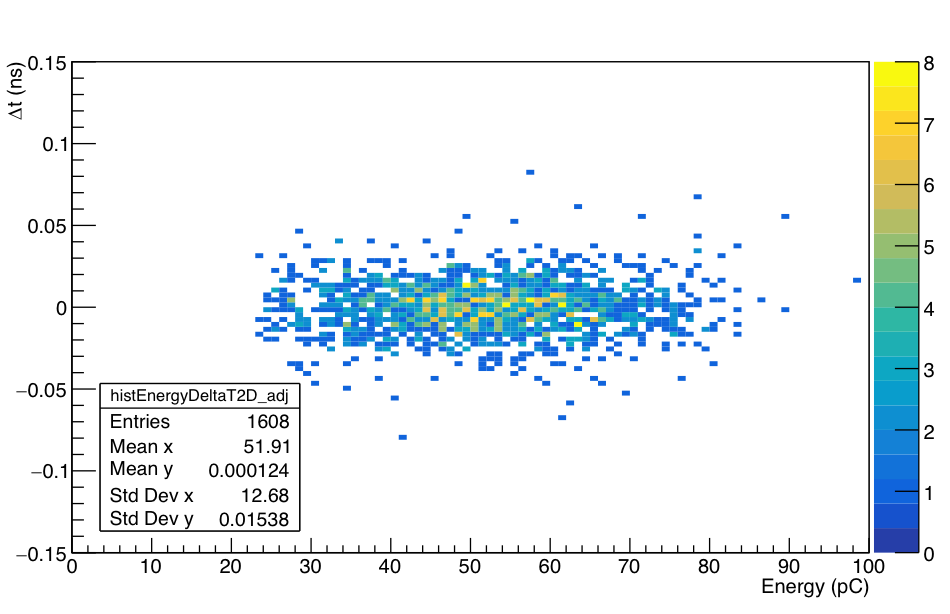
\includegraphics[width = 0.8\textwidth]{32_1mm_2dhist}
\caption{2D histogram of the $\Delta$ t value and the charge contained in an event, with the number of events indicated by the coloring.}
\label{2D histogram}
\end{figure*}

Once events are selected and the time resolution is determined, it is seen that as the event energy increases, the time resolution improves. The 32 and 16 GeV data have similar time resolutions for similar event charges, however, the 8 GeV data has a significantly larger time resolution. More data at intermediate beam energies is needed to fully understand these results, as these intermediate beam energies would have more events with similar energies than the current beam energies do. The points in Figure \ref{time res event energy} are plotted at the center of their charge cut range.

\begin{figure*}[!htbp]
\centering
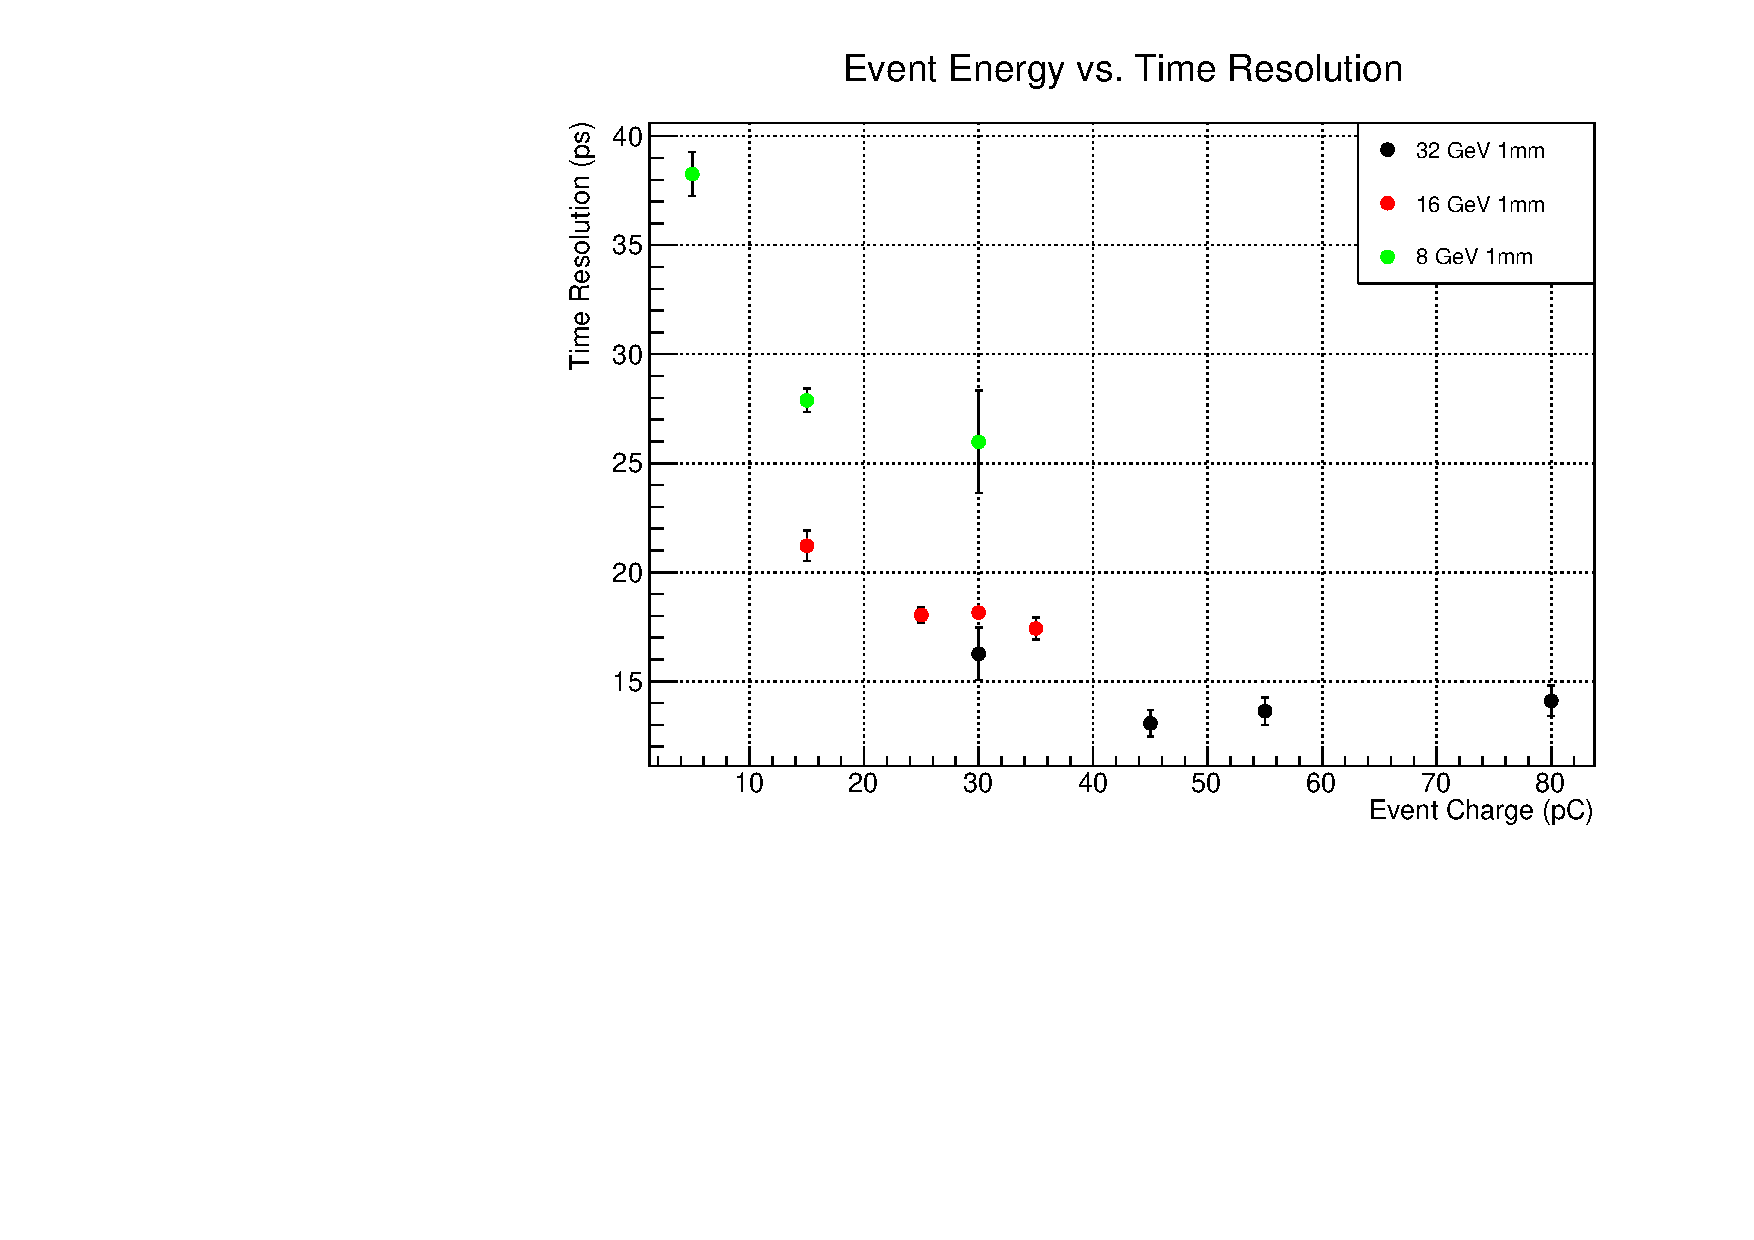
\includegraphics[width = 0.8\textwidth]{time_res_event_energy}
\caption{Time resolution determined by events selected in bins of event charge.}
\label{time res event energy}
\end{figure*}

\section{Analysis}

Overall, these results have shown that the pico-sil HGC detector achieves an outstanding time resolution of 16 ps at a beam energy of 32 GeV and a separation distance of 1mm between the absorber and the detector. Due to the shower shape being focused on the central pixel, combining pixels does not significantly improve the time resolution in the 32 GeV with a separation distance between the HGC and the absorber of 1, 10, 32, and 75 mm. For the case where pixels have very different time resolutions and contained charges, when pixels are combined, the time resolution is most improved with a charge weighting model.

When the SKIROC chip is modeled by adding 50 ps time smearing from numbers sampled from a Gaussian, it is found that pixel combination is advantageous. With 50 ps time smearing, equal weighting and charge weighting provide approximately the same time resolution improvement. The expected $\sqrt{N}$ time resolution improvement is not seen, as the central pixel is still dominating over the other pixels.

With 500 ps smearing, equal weighting provides a significantly better time resolution improvement than charge weighting does. With this large of a smearing, all pixels have approximately the same time resolution to begin with, so weighting each pixel equally makes sense. Additionally, with the 500 ps smearing, the expected improvement in time resolution proportional to $\sqrt{N}$ is seen, where $N$ is the average number of pixels with signal. This confirms that combining pixels with a similar time resolution improves the time resolution following the $\sqrt{N}$ relationship.

Overall, this demonstrates that 30 ps time resolution is achievable with the HGC detector and the SKIROC2 chip for digital signal conversion. This will allow for a spatial resolution of approximately 1 cm such that collision vertices can be correctly identified in a pile-up collision.

\section{Future}

More analysis at beam energies between 8 and 16 GeV, and between 16 and 32 GeV would help to understand the energy dependence of the time resolution and characterize this more accurately. Additionally, a better understanding of the time shift and dependence of the time resolution on event charge is needed, and more of the current data can be analyzed for this relationship.

\section{Acknowledgments}

I would like to thank my mentors Artur Apresyan, Javier Duarte, Cristian Pena, Maria Spiropulu, and Si Xie for supervising this project and providing feedback and guidance, both at Fermilab and Caltech. Many thanks to Jason Trevor and Dorian Kcira in the Spiropulu Group for their support and help also. 

Thanks to Daniel Gawerc who I have been collaborating on the analysis of the Fermilab test beam data with.

Additionally, I would like to thank the Caltech SURF Program and The Associates for providing funding for this work.

\newpage

\nocite{*}

\bibliographystyle{apsrev4-1} % Tell bibtex which bibliography style to use
\bibliography{GillianKopp/progress_report} 
\end{document}
